\documentclass
[
    paper = a4,
    pagesize,
    12 pt,
    oneside,                       % Chose ›oneside‹ for digital version, ›twoside‹ for printed version.
    open = right,
    DIV = calc,
    BCOR = 0 mm,                   % Binding correction. Only necessary for printed version. Depends on actual binding.
    bibtotoc
]
{scrbook}

% Do not change the following commands.
\newcommand*{\printTitle}{}
\newcommand*{\printAuthor}{}
\newcommand*{\printDateOfBirth}{}
\newcommand*{\printPlaceOfBirth}{}
\newcommand*{\printSubject}{}
\newcommand*{\myTitle}[1]{\renewcommand*{\printTitle}{#1}}
\newcommand*{\myName}[1]{\renewcommand*{\printAuthor}{#1}}
\newcommand*{\myDateOfBirth}[1]{\renewcommand*{\printDateOfBirth}{#1}}
\newcommand*{\myPlaceOfBirth}[1]{\renewcommand*{\printPlaceOfBirth}{#1}}
\newcommand*{\mySubject}[1]{\renewcommand*{\printSubject}{#1}}

\myTitle{High-level Visualization of Graph Algorithms}  % Change!
\myName{Julius Milian Severin}  % Change!
\myDateOfBirth{March~12, 1995}  % Change!
\myPlaceOfBirth{Berlin, Germany}  % Change!
\mySubject{{Graph Algorithms}{Visualization}}  % Change!
\advisorOne{Martin~S. Krejca}
\advisorTwo{Thomas Bl\"asius}
\myGermanTitle{Abstrahierende Visualisierung von Graph-Algorithmen}

\usepackage[utf8]{inputenc}
\usepackage[T1]{fontenc}
\usepackage[english]{babel}

\usepackage{graphicx}

\graphicspath{{Images/}}

\usepackage{pgf}

\usepackage							% Microtypography tuning.
[
	protrusion = true,
	expansion = false,
	tracking = true,
	kerning = true,
	spacing = false,
	babel = true
]
{microtype}							% http://ctan.mirrorcatalogs.com/macros/latex/contrib/microtype/microtype.pdf

\SetTracking[unit = space]{font = */*/*/sc/*}{25}   % Adjust kerning for small caps.

\SetExtraKerning[unit = space]		% Adjusted kerning for certain characters.
{
	font = */*/*/*/*
}
{
	: = {100, },
	; = {100, },
	? = {150, 150},
	! = {150, 150},
	: = {250, },
	; = {150, },
	? = {250, 250},
	! = {250, 250},
	» = { , -200},
	« = {-200, },
	› = { , -200},
	‹ = {-200, },
	– = {200, 250},
	— = {200, 250},
	@ = {200, 200}
}

\usepackage{booktabs}
\usepackage{breakurl}
\usepackage{emptypage}

\usepackage[bottom]{footmisc}
\usepackage{remreset}

\makeatletter
    \@removefromreset{footnote}{chapter}
\makeatother

\renewcommand*{\footnoterule}{\rule{0 pt}{0 pt}}
\deffootnote[1.2 em]{1.2 em}{0 em}{\makebox[1.4 em][l]{\textbf{\thefootnotemark}}}

\usepackage{xparse}

\DeclareDocumentCommand{\myfootnote}{o o o m}
{%
    \IfNoValueTF{#1}%
    {%
        \footnote{#4}%
    }%
    {%
        \IfNoValueTF{#2}%
        {%
            \kern #1 em\footnote{#4}%
        }%
        {%
            \IfNoValueTF{#3}%
            {%
                \kern #1 em\footnote{#4}\kern #2 em%
            }%
            {%
                \kern #1 em\footnote[#3]{#4}\kern #2 em%
            }%
        }%
    }%
}

\usepackage{titlesec}

\titleformat{\chapter}
    {\normalfont\rmfamily\huge\bfseries}
    {\thechapter}{1 em}{}

\titleformat{\section}
    {\normalfont\rmfamily\Large\bfseries}
    {\thesection}{1 em}{}

\titleformat{\subsection}
    {\normalfont\rmfamily\large\bfseries}
    {\thesubsection}{1 em}{}

\titleformat{\subsubsection}
    {\normalfont\rmfamily\normalsize\bfseries}
    {\subsubsectionname}{1 em}{}


\pagestyle{headings}

\usepackage{amsmath}
\usepackage{amssymb}
\usepackage{amsfonts}
%\usepackage{upgreek}               % Use if you want to use upright lowercase and italic upercase greek letters.
%\usepackage{dsfont}                % Use if you want to use special symbols.

%\usepackage[printonlyused]{acronym} % Use if you want to have acronyms. http://mirror.hmc.edu/ctan/macros/latex/contrib/acronym/acronym.pdf

%\usepackage{pifont}				% Special symbols.
%\usepackage{fourier-orns}			% More special symbols.
\usepackage{lettrine}

\usepackage{enumitem}
\usepackage
[
	format = plain,
	textfont = {sf, footnotesize},
	labelfont = {sf, bf}
]
{caption}[2008/08/24]
\usepackage{subcaption}				% For using sub-figures.

\usepackage
[
    algo2e,
    ruled,
    vlined,
    linesnumbered,
    algochapter
]
{algorithm2e}

\SetAlCapFnt{\sffamily\footnotesize}
\SetAlCapNameFnt{\sffamily\footnotesize}

\usepackage[numbers]{natbib}

\makeatletter
    \def\NAT@spacechar{~}% NEW
\makeatother

\definecolor{darkblue}{rgb}{0, 0, 0.5}

\usepackage
[
	bookmarks = true,
	bookmarksopen = false,
	bookmarksnumbered = true,
	pdfstartpage = 1,
	pdftitle = {{\printTitle}},
	pdfauthor = {{\printAuthor}},
	pdfsubject = {{\printSubject}},
	backref = page,
	breaklinks = true,
	colorlinks = true,
	linkcolor = darkblue,
	anchorcolor = darkblue,
	citecolor = darkblue,
	filecolor = darkblue,
	menucolor = darkblue,
	pagecolor = darkblue,
	urlcolor = darkblue
]

\usepackage{hyperref}


\renewcommand*{\backref}[1]{}
\renewcommand*{\backrefalt}[4]
{
    \ifcase #1
        Not cited.
    \or
        \footnotesize (Cited on page #2.)
    \else
        \footnotesize (Cited on pages #2.)
    \fi
}

\usepackage{cleveref}

\begin{document}




\begin{document}


\frontmatter
% Title Page
\thispagestyle{empty}
\begin{center}
    {\Huge \textbf{\printTitle}}\\[7 ex]
    {\Large\textsc{Bachelor Thesis}}\\[4 ex]    
    {\large
        to attain the scientific degree\\[4 ex]
        \textbf{Bachelor of Science}
    }
    \vfill
    \includegraphics[width = 8 cm]{HPI_logo.pdf}\\[8 ex]
    \begin{tabular}{l}
        handed in by \textbf{\printAuthor}\\[1.1 ex]
        born \printDateOfBirth, in \printPlaceOfBirth\\[3 ex]
        \textbf{Advisor:} Prof.~Dr.~Tobias Friedrich\\[9 ex]
    \end{tabular}
    
    Potsdam, \today
\end{center}

% Abstract
\chapter*{}
\addcontentsline{toc}{chapter}{Abstract}
\thispagestyle{empty}

\begin{center}
    \large \textbf{Abstract}
\end{center}

Developing an algorithm is an iterative process.
Therefore an understanding of the different approches is important.
Furthermore, as the algorithm becomes more complex, it may come to different results than expected, when running on real data.

This thesis deals with those issues on the example of shortest path algorithm on tiled map data.
Therefore, multiple ways of visualizing a shortest path algorithm with respect of this specific class of algorithms are introduced.
Using those methods we were able to archieve a better understanding of the algorithms and built a powerful basis for discussions.
In addition we enabled the researchers to find the missbehaviour more easily.

\chapter*{}
\addcontentsline{toc}{chapter}{Zusammenfassung}
\thispagestyle{empty}

\begin{center}
    \large \textbf{Zusammenfassung}
\end{center}

Das Entwickeln eines Algorithmusses ist ein iterativer Prozess.
Daher ist es wichitg, dass alle Beteiligten, die verschiedenen Ansätze verstehen.
Ausserdem kann es mit wachsender Komplexität des Algoithmus dazu kommen, dass sich der Algorithmus auf echten Daten anders verhalten als gedacht.
Das finden der Ursache kann ein äußerst komplexes Verfahren sein.

In der folgenden Arbeit erklären wir, wie wir die Entwicklung eines Algorithmus zum finden kürzester Wege durch eine Visualisierung untersützt haben.
Dabei gehen wir auf die Probleme ein, die wir wärend der Entwicklung der Visualisierung lösen mussten.


% Table of Contents
\renewcommand*{\listfigurename}{\normalfont\rmfamily\Large\bfseries List of Figures}
\renewcommand*{\listtablename}{\normalfont\rmfamily\Large\bfseries List of Tables}
\pdfbookmark{\contentsname}{toc}
\microtypesetup{protrusion = false}
    \tableofcontents
    \begingroup
    \let\clearpage\relax
    \listoffigures                  % Comment out if necessary.
    \listoftables                   % Comment out if necessary.
    \endgroup
\microtypesetup{protrusion = true}


\mainmatter
\chapter{Introduction} \label{introduction}
% Algorithmen
Graphs are a common structure in computer science.
Therefore, developing more efficient graph algorithms plays a big role in algorithm engineering.

% Visualisierung
During the process of development knowing how the algorithm behaves is really important.
As developing an algorithm is an iterative process it is fundamental to communicate about the different approaches and therefore create an understanding of them in the whole team.
Furthermore, the developed algorithms can become quite complex and therefore the idea of how the algorithms should behave and the way they actually behave on real graph data can diverge quite a lot.

% Projekt
In the last year, we developed a shortest-path algorithm on geographical tiled map data.
The tiles impact the algorithm insofar that the loading of a tile has high costs and should therefore be done as little as possible.
A tile needs to be loaded whenever a node of the tile is processed.
As the algorithm was developed for portable devices, it has access to the so-called cache: a fast storage.
The cache can store a limited amount of tiles.
Therefore a tile does only need to be loaded whenever it is not in the cache.
Due to the limited size of the cache, loading a tile into the cache, requires removing another, as soon as the cache is full.

As the eyes are a fast way to access information, we decided to visualize the progress of the algorithm to achieve the necessary understanding.
Though there are many tools for visualizing graphs, there is a lack of algorithm visualization tools, which might result from the high amount of individual characteristics of algorithms and their underlying graph.
Therefore developing an own visualization that fits one's individual needs is necessary.

In the following we are going to explain different approaches we developed for the specific class of algorithms.
In \Cref{questions}, we are going to motivate different methods to display the algorithm.
In the following \Cref{main} those methods are then introduced, explained and discussed based on the structure given by \Cref{questions}.


\chapter{Preliminaries} \label{questions}

In this chapter, we will first introduce the algorithms that the visualization is going to display.
Then, we will touch upon the graph data the algorithms are running on.
Thereupon, the characteristics of the visualization are presented.
The implementation of those characteristics is then discussed in \Cref{main}.


\section{Problem Specification} \label{specification}

This section will present the scope the visualization is runnging in.
Therefore in \Cref{framework} we are going to introduce the algorithms that are going to be displayed and in \Cref{spec_graph} the underlying graph is described.

\subsection{The Class of Algorithms} \label{framework}

The visualization we built has the purpose of visualizing shortest path algorithms.
A shortest path algorithm, in general, has the goal to find the path with the lowest summed weight from a given start node to a given target node in a weighted graph.

The class of algorithms is based on Dijkstra's algorithm\cite{DIJKSTRA1959} and its improvement, the A*-algorithm\cite{4082128}.
Dijkstra's algorithm starts at the start node wherefrom it adds the neighbors of the node to a priority queue that orders the elements by their distance to the start node.
In each iteration, the node with the highest priority (smallest distance) is removed from the queue and its neighbors are added to the queue, when not already inserted.
Whenever the node that is going to be removed from the queue is the target node, the shortest path is found.
This results in a uniformly spreading of the search space around the start node.

The A*-algorithm generally adopts this strategy.
Its goal is to search target oriented and therefore reduce the search space.
Therefore the queue of the A*-algorithm is ordered not only by the summed distance of the edges to the start node but also by the linear distance to the target node.
Thereby nodes presumably closer to the target get expanded first.
This leads to a target directed spreading.

At this point, it is important to notice that both algorithms create a coherent area of processed nodes.

\subsection{The graph} \label{spec_graph}

The underlying graph of the algorithms is a real-world road network.
Every node has given coordinates that refer to a certain position on  Earth, the edges are directed and the weight of an edge can be calculated using its speed and its length.
Special about the graph is, that it is based on the Navigation Data Standart (NDS).
Based on the NDS the graph is split into tiles according to a geographical grid.

This impacts the algorithms in so far, that accessing tiles becomes the major effort on runtime, as the tiles are encrypted and compressed.
Hence the algorithms should access as little tiles as possible.
As the algorithms are developed for portable devices, they have access to the so-called cache: a fast storage with limited size.
Since tiles can be stored in the cache, accessing a tile is only costly whenever it is not in the cache.
A tile is \emph{accessed} whenever a node of the tile is processed.
Due to the limited size of the cache, loading a tile into the cache requires removing another, as soon as the cache is full.


\section{Basic Elements}

In \Cref{graph}, we introduce the representations of basic elements of the graph.
We will discuss how to represent nodes, edges, and tiles in a meaningful way.
For the nodes, it is important to consider how they can be arranged on the screen, or rather discuss how to map the coordinates on the spherical Earth onto a plane.
For the edges, a method is introduced that integrates the the length and the speed in the representation.


\section{Displaying the Algorithm}

In \Cref{algorithm}, we describe how a basic visualization can be build.
With this foundation, we explain a method to display the cache and introduce multiple features for a better accessibility of information.


\subsection{Basics}

In \Cref{basic}, we describe how we can combine the elements from \Cref{graph} to build a basic visualization.
A main challenge here is to transform a static graph in a dynamic visualization that outlines the changing states of the graph during the ongoing algorithm.


\subsection{Visualizing the Cache} \label{pre_cache}

Based on the basic visualization build in \Cref{basic}, we present a way to make information about the state of the cache comprehensible in \Cref{cache}.
Then we introduce a method that enables us to see how well an algorithm performs regarding to the amount of tile loads, at any point of the visualization.


\section{Comparing Algorithms}

To see a progress in the development and examine an iteration of the algorithm, it is necessary to compare different algorithms based on the visualization.
Therefore a trivial strategy is to put two visualizations next to each other.
This approach did not produce the desired effect and therefore we introduce some other approches to compare algorithms.


\section{Miscellaneous}

Based on the developed high-level visualization, we will introduce additional features we added for a better accessibility of information.


\section{Run-Time Visualization vs. Post-Execution Visualization}

There are two possibilities of visualizing an algorithm.
One is to visualize the algorithm and what it does on runtime.
A second approch is to run the algorithm first and create log files from which, once the algorithm has finished, the visualization is created.

Run-time visualizations have the benefit that the algorithm does not have to be finished before things are visualized.
Therefore they are especially useful, whenever algorithms need a long time to finish.

Post-execution visualizations, on the one hand, need to wait till the algorithm is finished and the algorithm has to write the information the visualization needs in log-files which requires extra storage.
On the other hand they can display information the algorithm does not have yet, but increase the comprehensibility.

Most methods introduced in \Cref{main} are not limited to a specific kind of visualization, but some use information that are not given on runtime yet.

% The decision which kind of visualization to use needs to be reached with respect to some factors.
% In the case of our shortest path algorithm, the execution time is below half a minute in most cases and the storage is not such a big issue.
% On the other side some approaches we introduced are not possible using the run-time visualization.
%Therefore we prefer the post-execution visualization over the run-time visualization.


\section{The HSV Color Model}

The HSV Color Model describes a color by its hue, its saturation and its value.
\begin{itemize}
  \item Hue: The hue stands for the position of the pure color on the color wheel and therefore has a value between $0^\circ$ and $360^\circ$.
  \item Saturation: The saturation describes the colorfulness. Thereby it is indicated by a value between 0 and 1 whereby 0 reults in white and 1 in the pure color.
  \item Value: The value is similar to the saturation but instead of white a value of 0 results in black.
\end{itemize}

\begin{figure}[H]
  \begin{minipage}{\textwidth}
    
\includegraphics[width=\textwidth]{Images/hsv.png}
    \quelle{\cite{hsv}}
    \caption[]{Color gradient of HSV with hue values from $0^\circ$ on the left to $360^\circ$ on the right. As we only want to see the pure color the saturation and the value are 1.}
    \label{fig:hsv}
    \end{minipage}
\end{figure}
\todo{source of images}

Due to the hue that specifies the pure color on the color wheel, the HSV color model is a good choice whenever a smooth color transition is wanted, as we see in  \Cref{fig:hsv}.

\chapter{Building the Visualization} \label{main}

In this chapter, we will build the visualization and discuss the methods announced in \Cref{questions}.

\section{Basic Elements} \label{graph}

\paragraph{Nodes.}
Mapping coordinates of the spherical Earth to a plane is an extensively discussed topic, as it is needed for geographical maps and has its origin in the late 7th millennium BCE \cite{wiki:cartography}.
\todo{andere quelle}
For our visualization, we considered two known projections.

First, the Equirectangular projection which suggests itself due to its simplicity.
The other method is the Mercator projection that is one of the most common projections, as it is seen on most world maps and is also used by big map providers like Google maps \cite{google_maps}
It was originally developed for nautical cartography in the 16th century \cite{mercator}.

The Equirectangular projection is also known as unprojected map \cite{equirectangular}.
This is because it does only map the Earth on a plane by using the longitude as horizontal coordinate and the latitude as the vertical coordinate.
As the geographical distance between the longitudes shrinks the more the latitudes get closer to the poles, the projection is distorted in those areas.

The Mercator projection firstly maps the Earth as the Equirectangular projection does, but to prevent the distortion near the poles the Mercator projection stretches the map vertically in the affected areas.

\begin{figure}
  \begin{minipage}{\textwidth}
    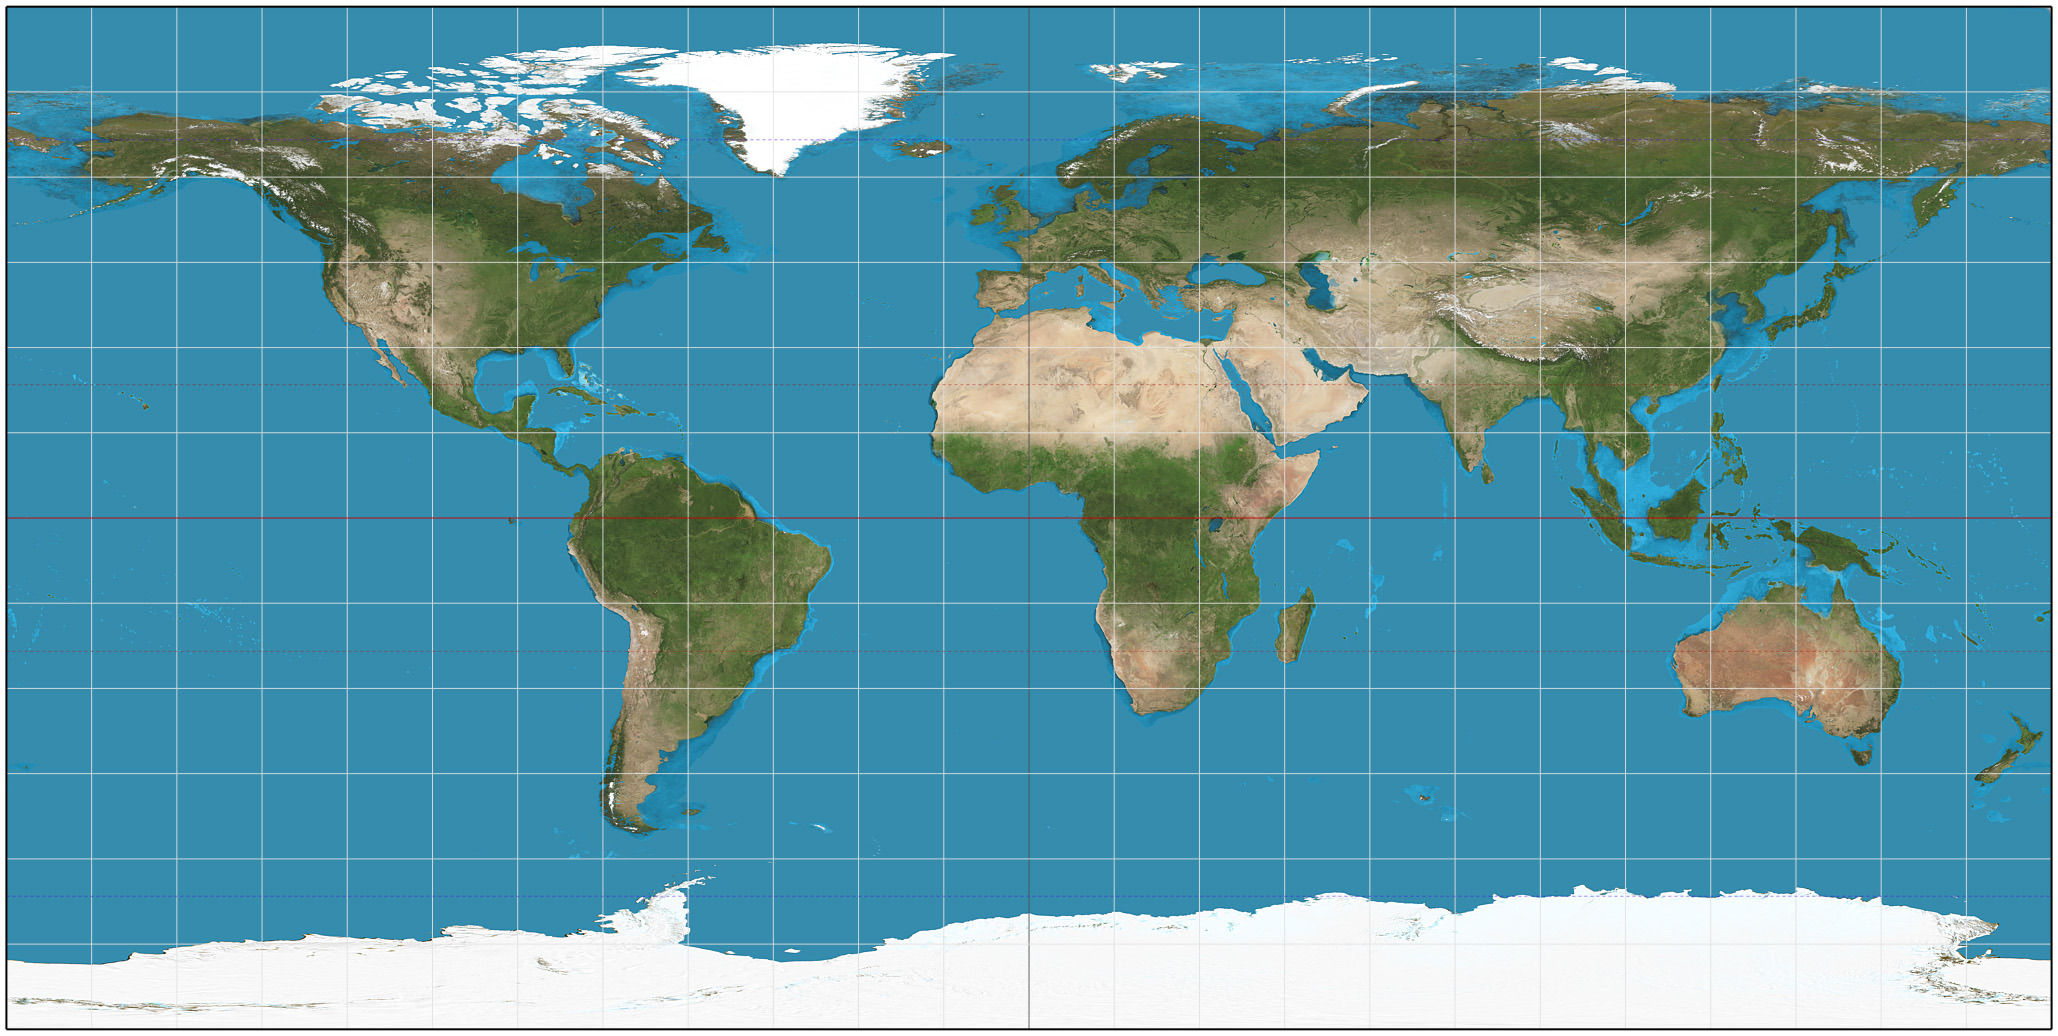
\includegraphics[width=.5\textwidth]{Images/Equirectangular_projection_SW.jpg}
    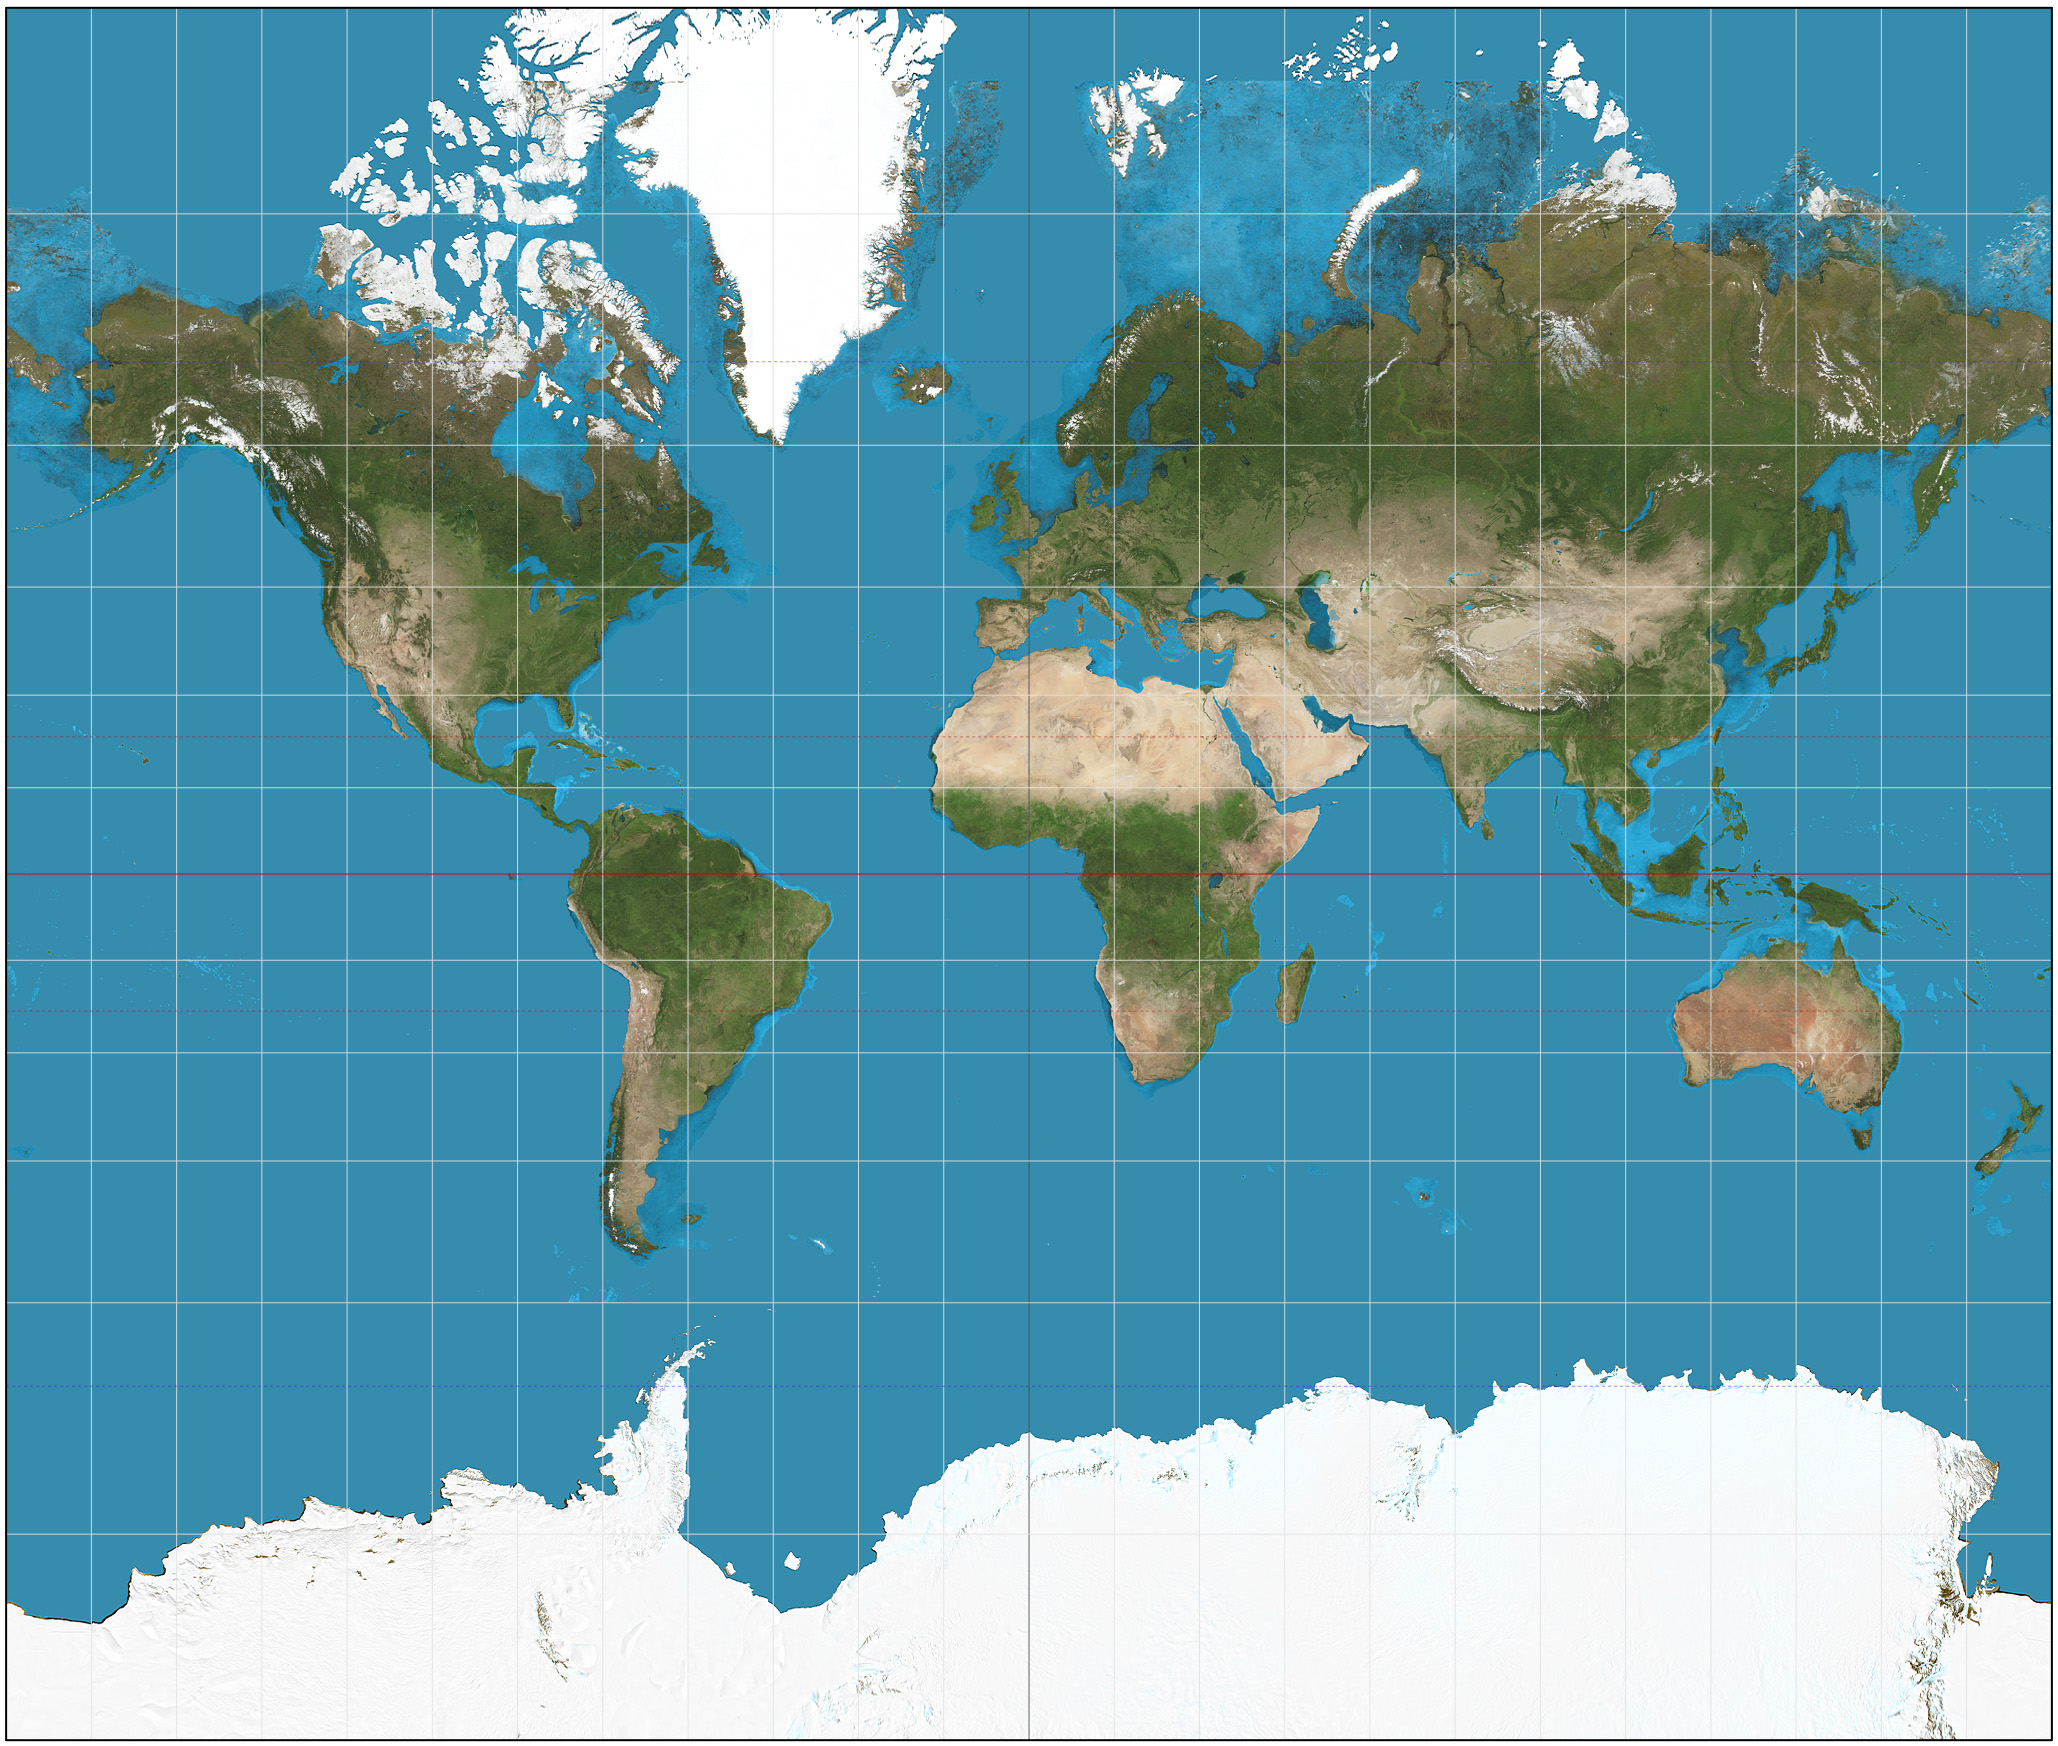
\includegraphics[width=.5\textwidth]{Images/Mercator_projection_SW.jpg}
    \quelle{\cite{mercator,equirectangular}}
    \caption[]{A map of the Earth mapped by the Equirectangular projection (left) and the Mercator projection (right). }
    \label{fig:projections}
  \end{minipage}
\end{figure}
\todo{source of images}

In \Cref{fig:projections} we can see, what we already described before.
In contrast to the Equirectangular projection on the left that looks quite swaged near the poles, the Mercator projection on the right stretches vertically in those parts, which leads to a much more natural looking map.

Nevertheless, the Equirectangular projection has the huge benefit, that we can use the given coordinates without any additional calculations.
For the Mercator projection, it is required to apply a formula to each coordinate displayed.
Therefore, and due to the fact that the effect of the Mercator projection is quite low in most areas and particularly those that we are going to display, we decided to use the Equirectangular projection for our visualization.

For the representation of nodes circles are a common element and widely seen in graph visualizations, but as those visualizations are mostly used for smaller graphs, usually to explain the basic concepts of an algorithm and we were going to display graphs with millions of nodes, we had to reconsider this representation of nodes.
As we know that at the end of every edge is exactly one node, we can clearly identify every node, as long as the node is connected to any other edge.
Therefore we decided to not use any additional representation of nodes to the visualization, as they do not add any value to it and only make the visualization more crowded.
We notice that we do not display nodes that are not connected to any other node.
As the only way for those nodes to play a role during the algorithm is be to be the start or the target node, the absence of those nodes is reasonable.

\paragraph{Edges.}

A common approach for dipplaying edges is to represent them by straight lines.
The length of the edges is in general reflected by the length of the lines in most cases.
However, we need to respect, that it is possible, that the linear distance of two nodes, which is displayed by the linear representation, can diverge quite a lot to the real length of the edge in some cases.
In addition, as we use the Equirectangular projection, the lines are distorted horizontally dependent on their distance to the poles.

In order to represent the speed of an edge as well, we can color the edges according to their speed.
By using the HSV color space we achieved a seamless color transition from red for 0 km/h, yellow for a speed of about 60 km/h and green for the fastest edges with a speed of 120 km/h and more.
Using HSV we are be able to outline edges with a speed of 240 km/h without any issues in understandability.


\paragraph{Tiles.}
One way of visualizing the tiles, that does not require any new element is, to show all edges of the tile in a lighter color as soon as the tile is accessed the first time.
This representation has the disadvantage that it is only possible to distinguish tiles at the outer graph.

By using rectangles to outline the tiles it is possible to differentiate tiles at every region of the graph.
Due to the Equirectangular projection, all those rectangles have the same size and are, as in the previous method displayed at their first access.


\section{Displaying the Algorithm} \label{algorithm}

In this section, we describe how we used the elements, introduced in \Cref{graph} for displaying how the graph evolves during the ongoing algorithm.

\subsection{Basics} \label{basic}

\paragraph{Combining the Elements.}

For a basic edge-based visualization we start with an empty space and then add one edge after another as they are processed by the algorithm.
This will happen either automatically or on request by pressing a key.

For now, we assume displaying the correct region of the graph is not a problem.

\begin{figure}
    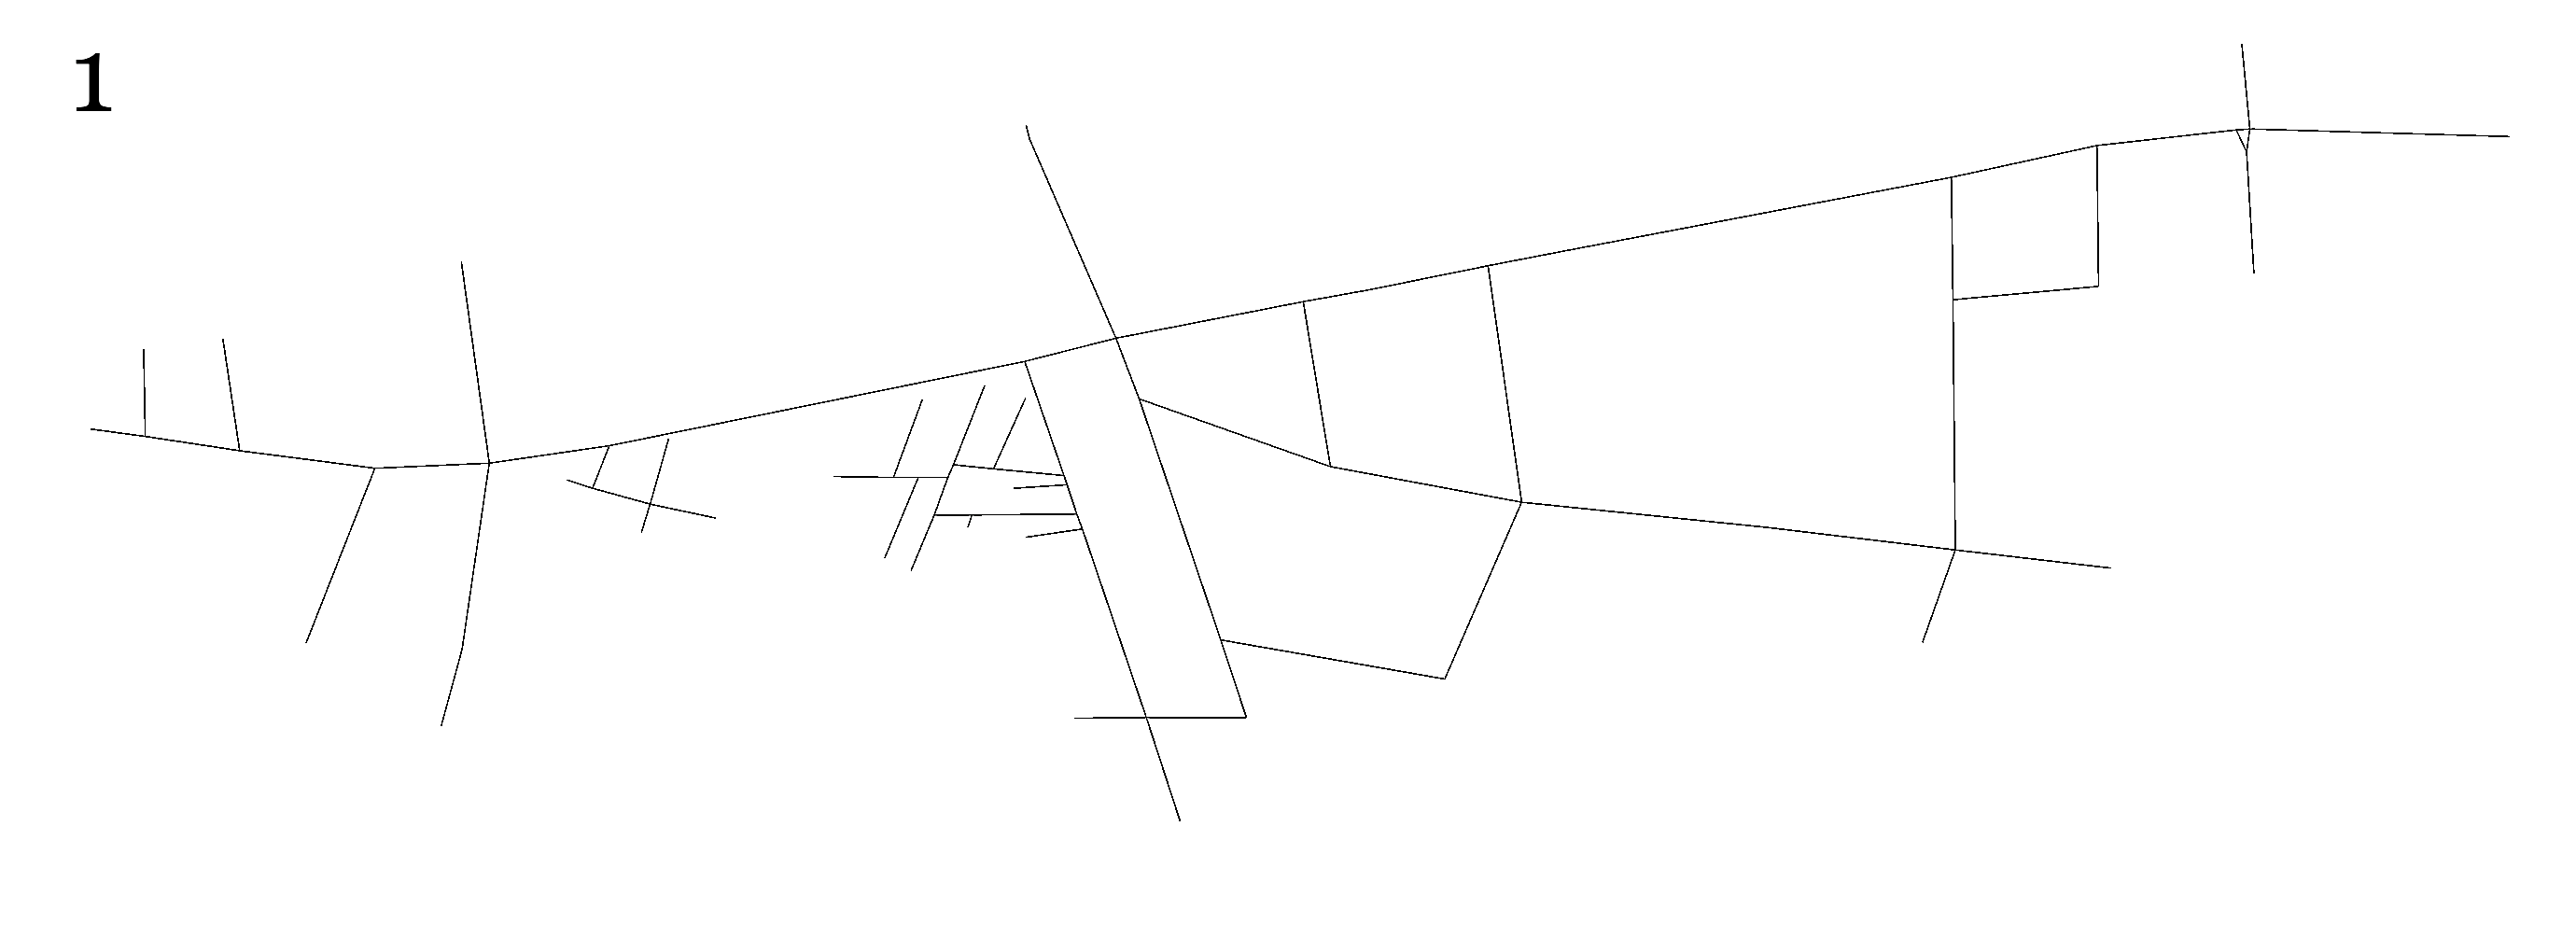
\includegraphics[width=.5\textwidth]{Images/vis-step-one.png}
    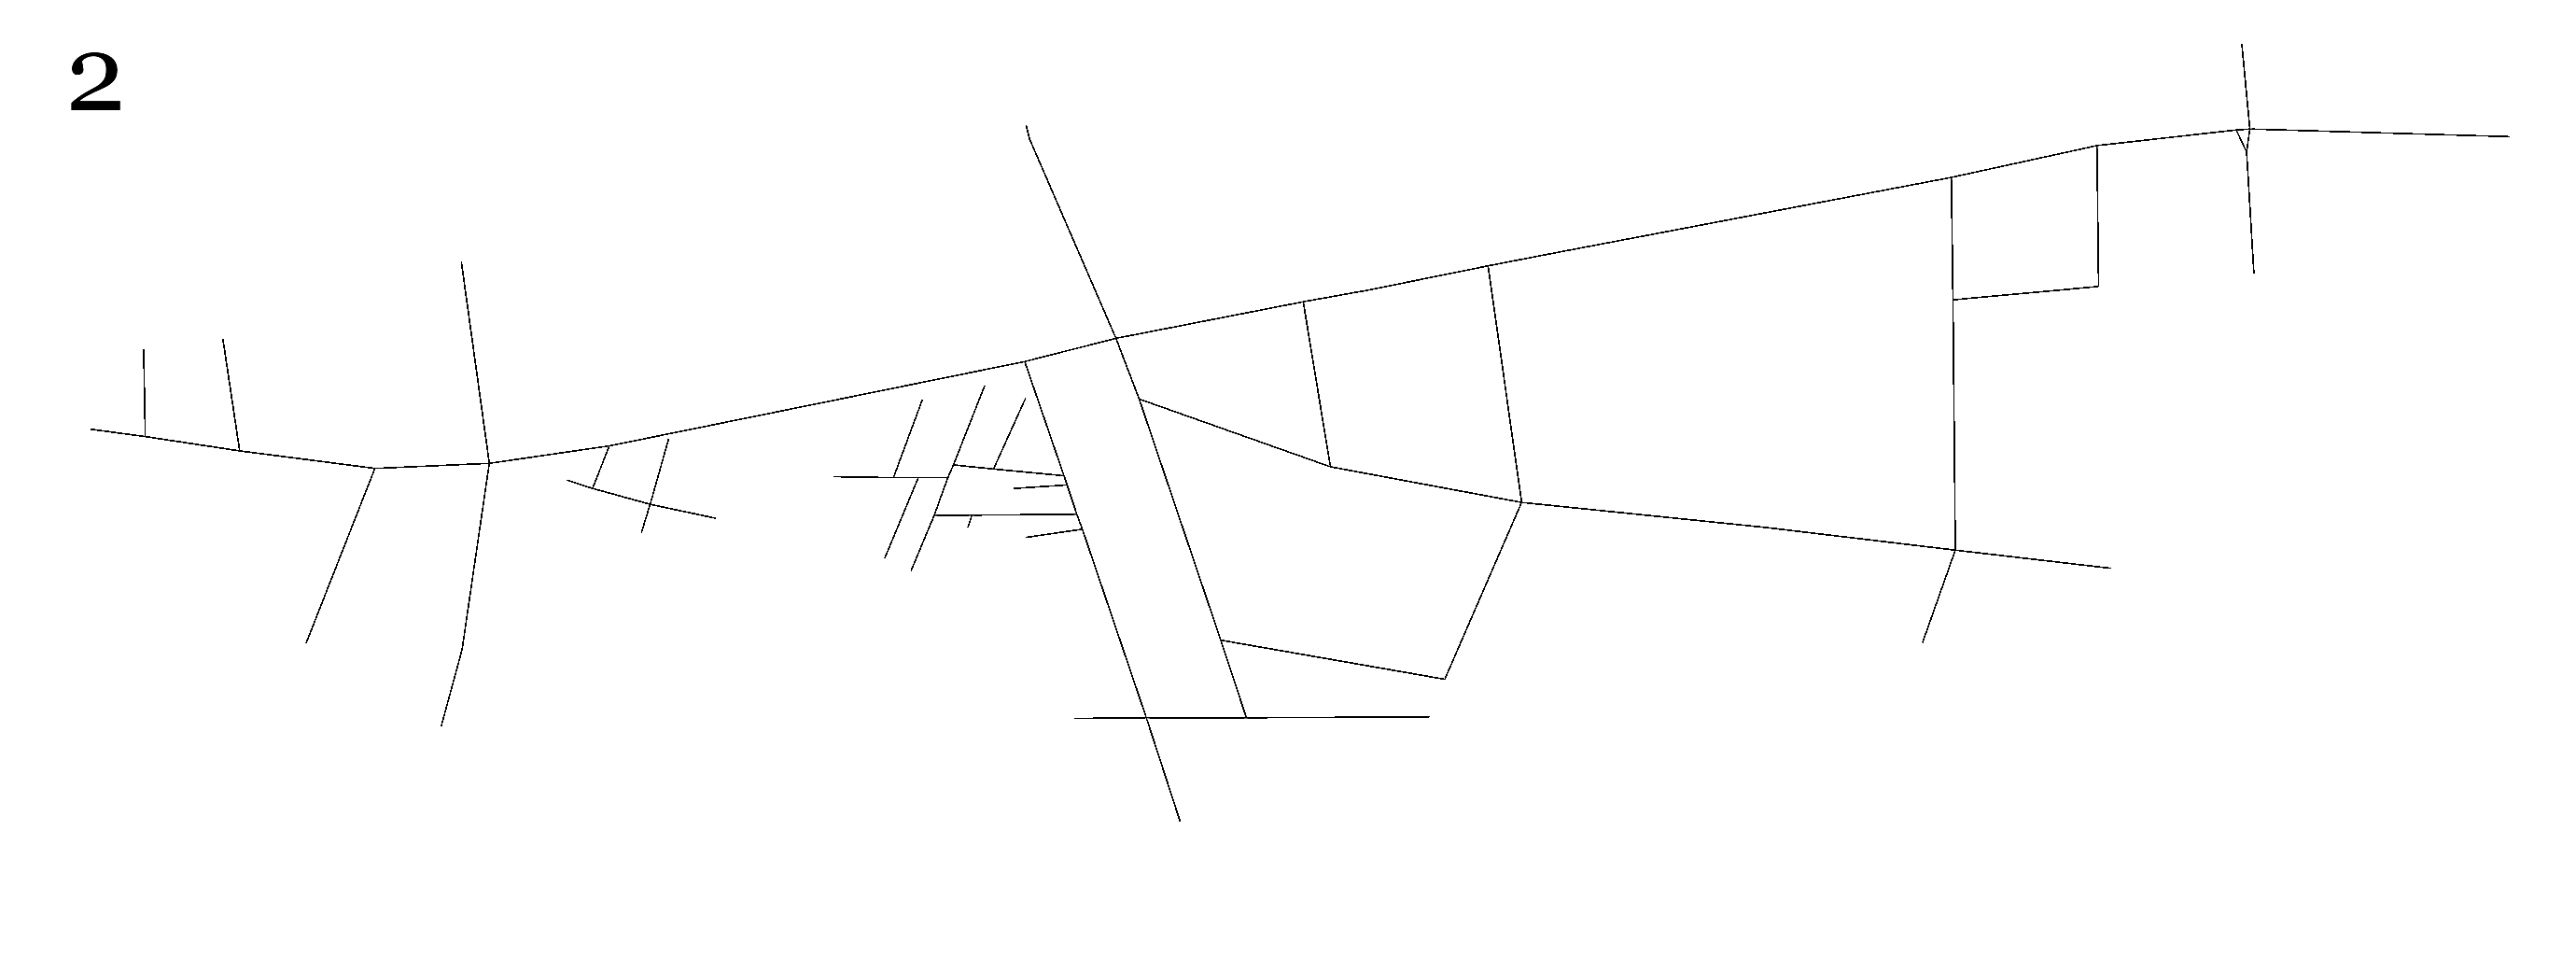
\includegraphics[width=.5\textwidth]{Images/vis-step-two.png}
\caption{Two consecutive steps in the visualization. Every black line represents an edge.}
\label{fig:two-steps}
\end{figure}
\todo{auflösung}

In \Cref{fig:two-steps} we can see that we got a good basic understanding of how the algorithm evolves.
The tiles can be visualized on a similar way.
A tile is alway displayed whenever its first edge is processed.

\begin{figure}
    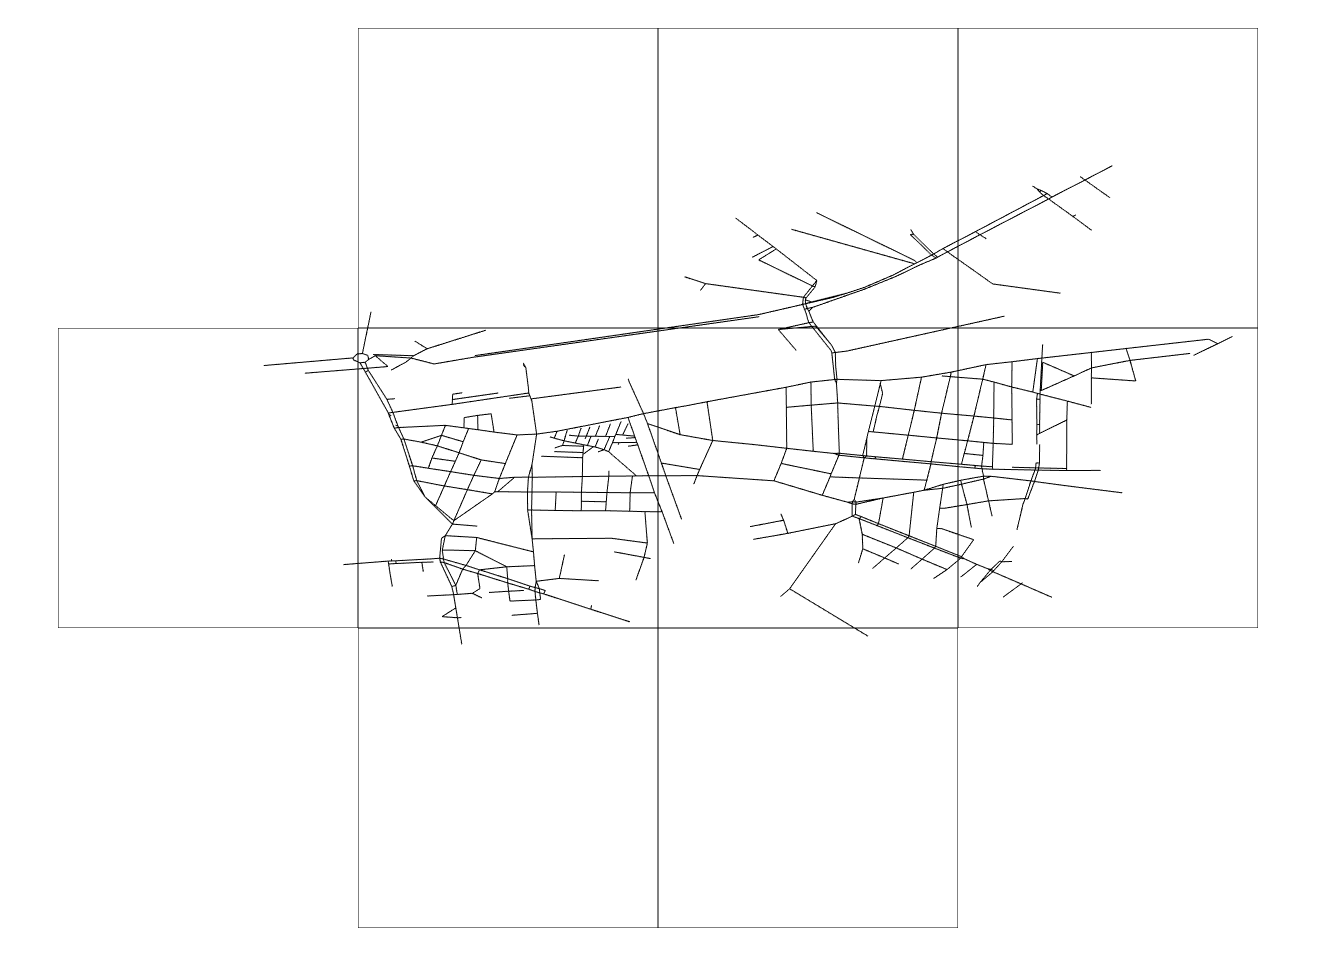
\includegraphics[width=\textwidth]{Images/vis-rectangular-tiles-small.png}
\caption[]{Extension of \Cref{fig:two-steps}. In addition tiles are represented by rectangles.}
\label{fig:rectangle_tiles}
\end{figure}

The strategy of displaying edges and tiles as seen in  \Cref{fig:rectangle_tiles} works great on smaller routes and it is possible to track the state of the algorithm quite good.

\begin{figure}
    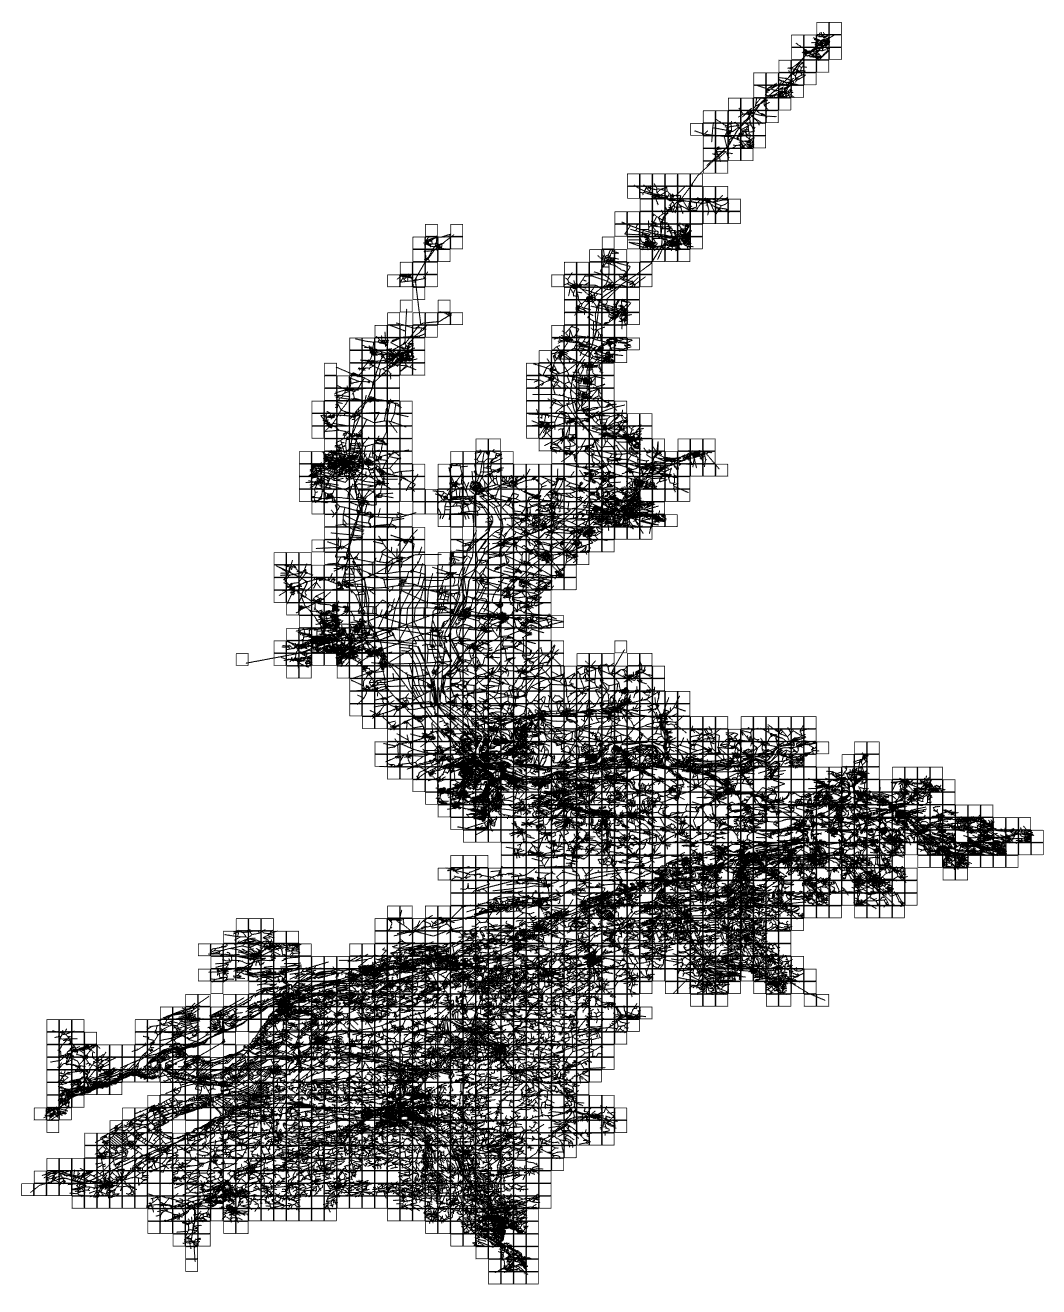
\includegraphics[width=\textwidth]{Images/vis-rectangular-tiles.png}
\caption[]{Using the same method as in \Cref{fig:rectangle_tiles}, but on a bigger route.}
\label{fig:rectangle_tiles_big}
\end{figure}
\todo{bessere auflösung}

On bigger routes, however, this visualization lacks in comprehensibility as we can see in \Cref{fig:rectangle_tiles_big}.
In addition, we experienced performance issues due to the amount of displayed elements and one step is hard to distinguish from its predecessor.
Thus, for longdistance queries, it makes sense to remove the edges from the visualization.

\begin{figure}
        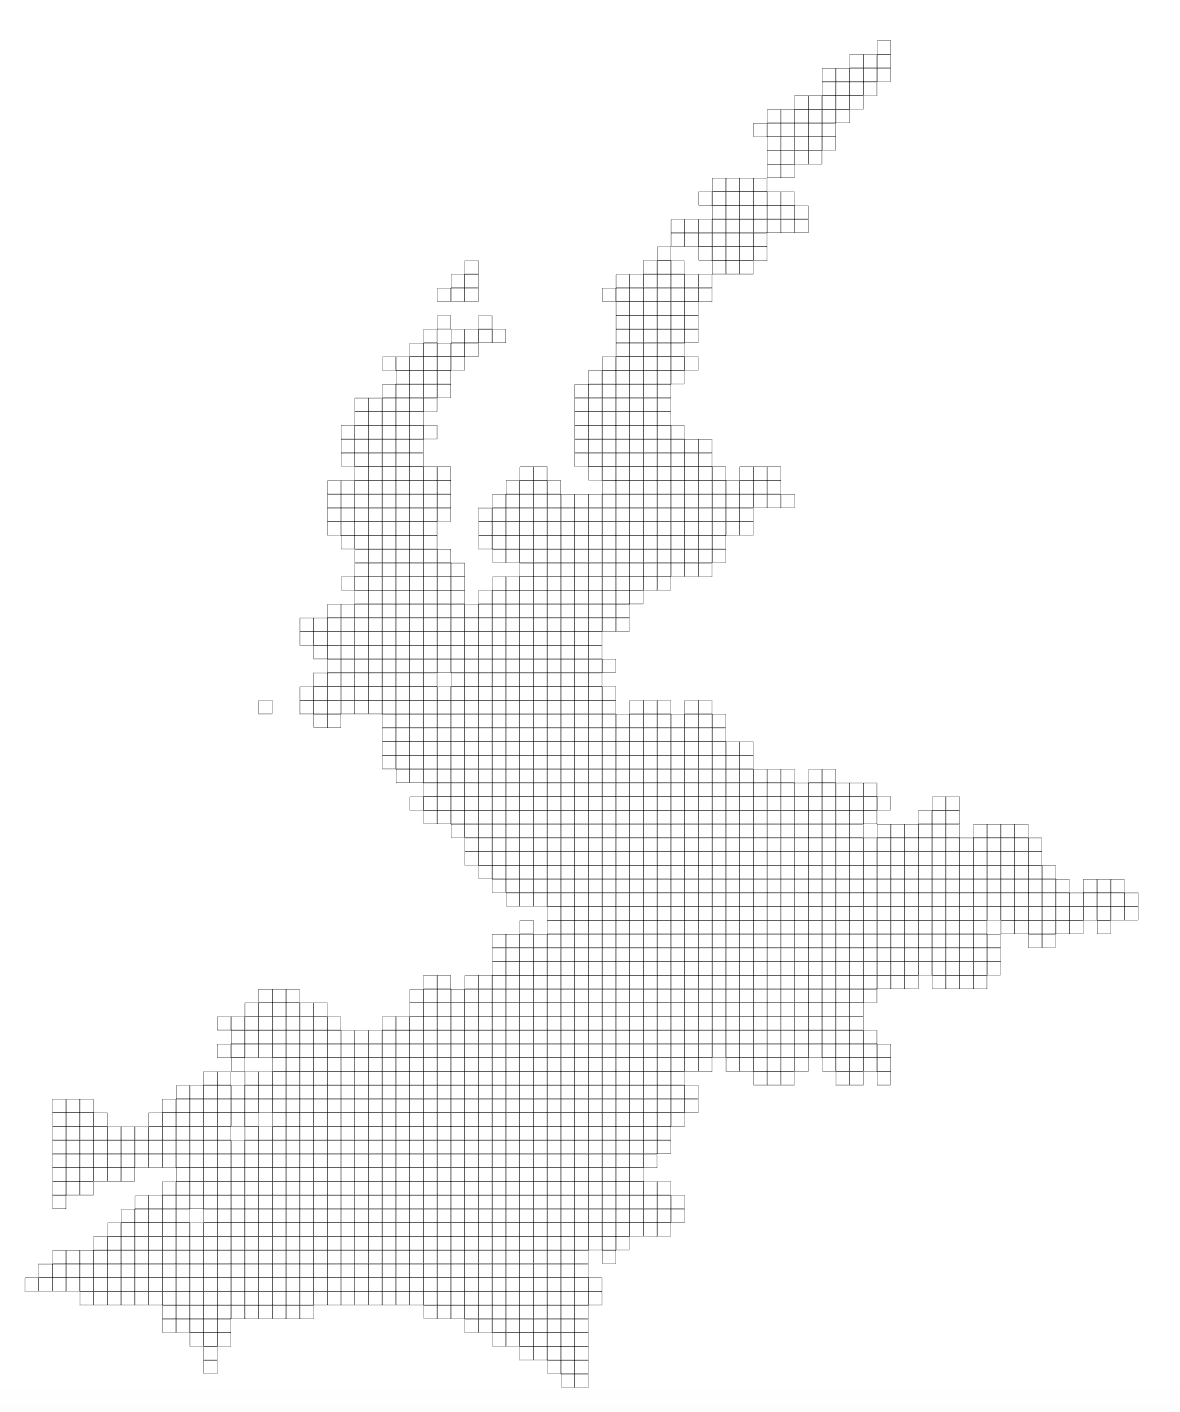
\includegraphics[width=\textwidth]{Images/vis-only-rectangles.png}
\caption[]{Representing tiles only through rectangles.}
\label{fig:only_rectangles}
\end{figure}

In \Cref{fig:only_rectangles} we see an uncluttered representation based on tiles.
By removing the edges we also experienced a tremendous performance boost.


\paragraph{Outlining the Current Step}

In the tile-based visualization, we can see in \Cref{fig:only_rectangles}, it is hard to recognize whenever a tile is added to the graph.
Furthermore, it is impossible to notice which tile the algorithm is currently processing.
Therefore a trivial approach is to color the tile in which edges are currently processed.

For adding an understanding about which route the algorithm is going to find and the possibility to see how far the algorithm already proceeded to find the path, we added the resulting path of the algorithm to the visualization.
This is, of course, only possible when the visualization is executed after the algorithm has finished.

\begin{figure}
        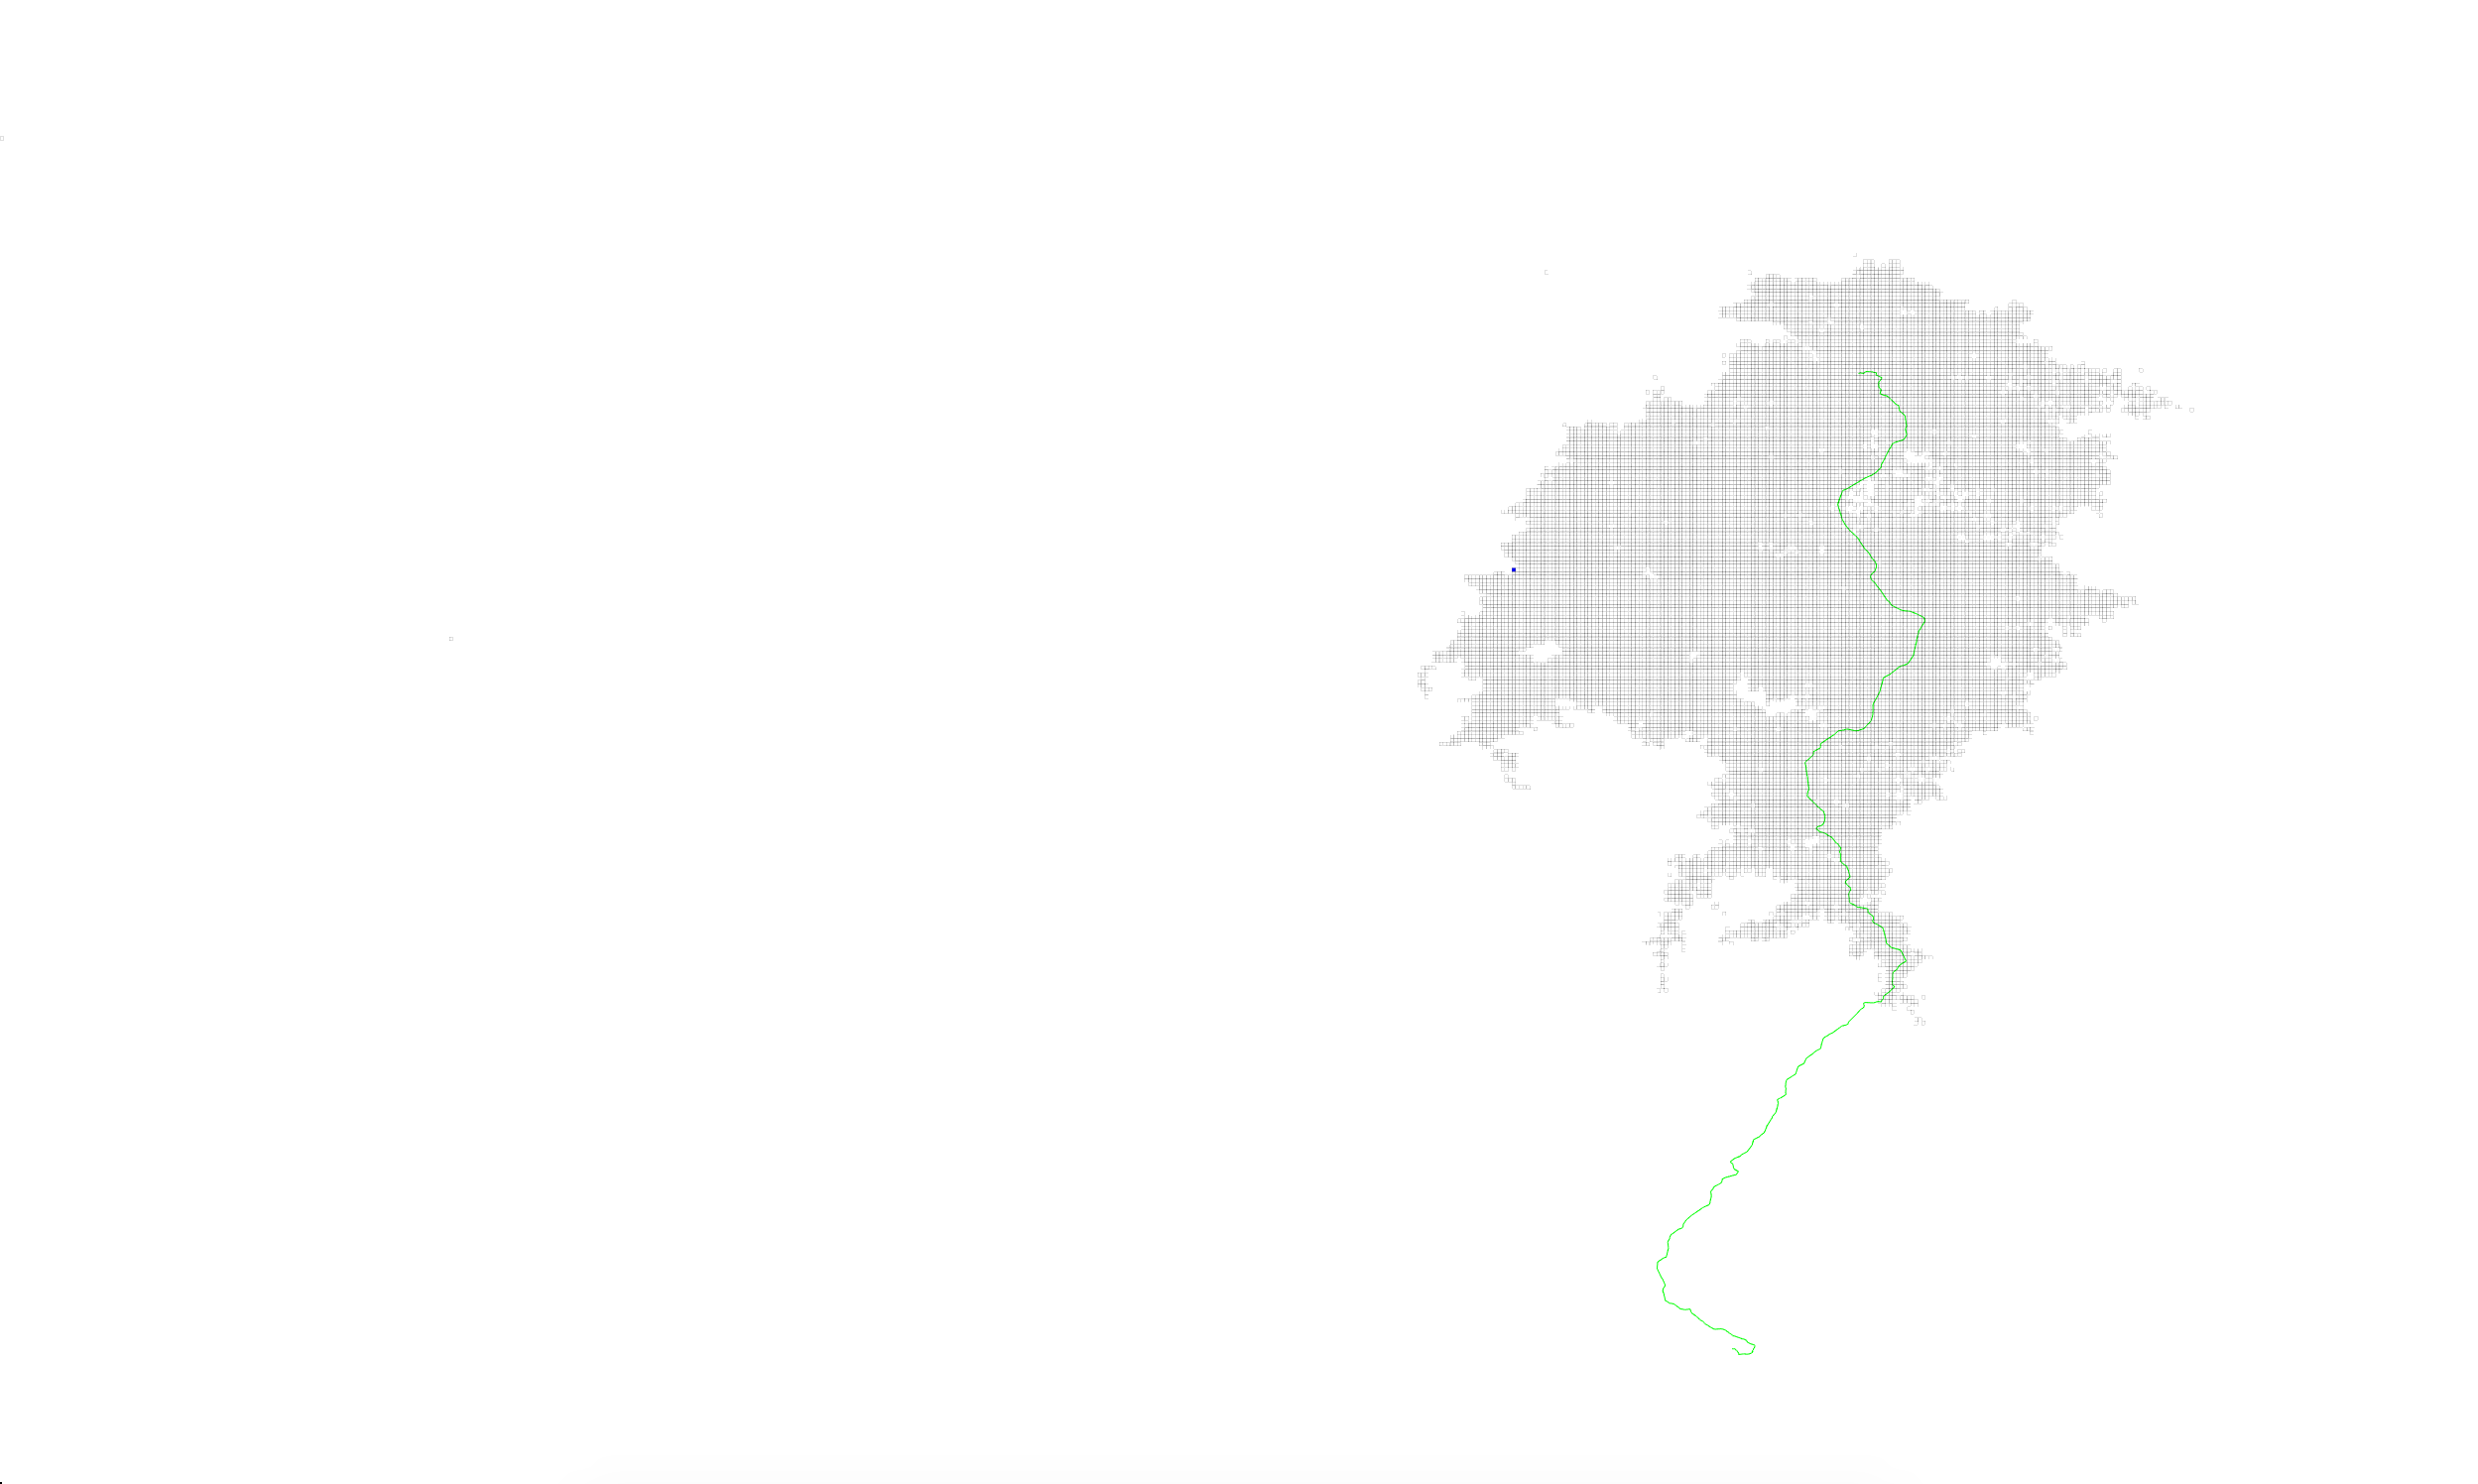
\includegraphics[width=\textwidth]{Images/vis-current-tile.png}
\caption[]{Coloring the tile that is processed blue. The searched path is represented in green.}
\label{fig:color_current_tile}
\end{figure}

Even though this method enables us to see which tile is processed in a single image, the information gain of this feature is quite small, as we can see in \Cref{fig:color_current_tile}.
For learning something about the algorithm, knowing what tile is loaded in one specific step is not enough.
Rather knowledge about many successive steps is needed.
This could be achieved by just running the visualization, but when doing this the colored tile is only hardly visible.
Thus we had to figure out a more compatible method of showing what is going on.

We came up with a method we called aging of tiles.
This method builds on the previously introduced method, but instead of uncoloring the tile immediately, it uncolors it over time.
Therefore the tile becomes a bit brighter every step of the algorithm.

\begin{figure}
    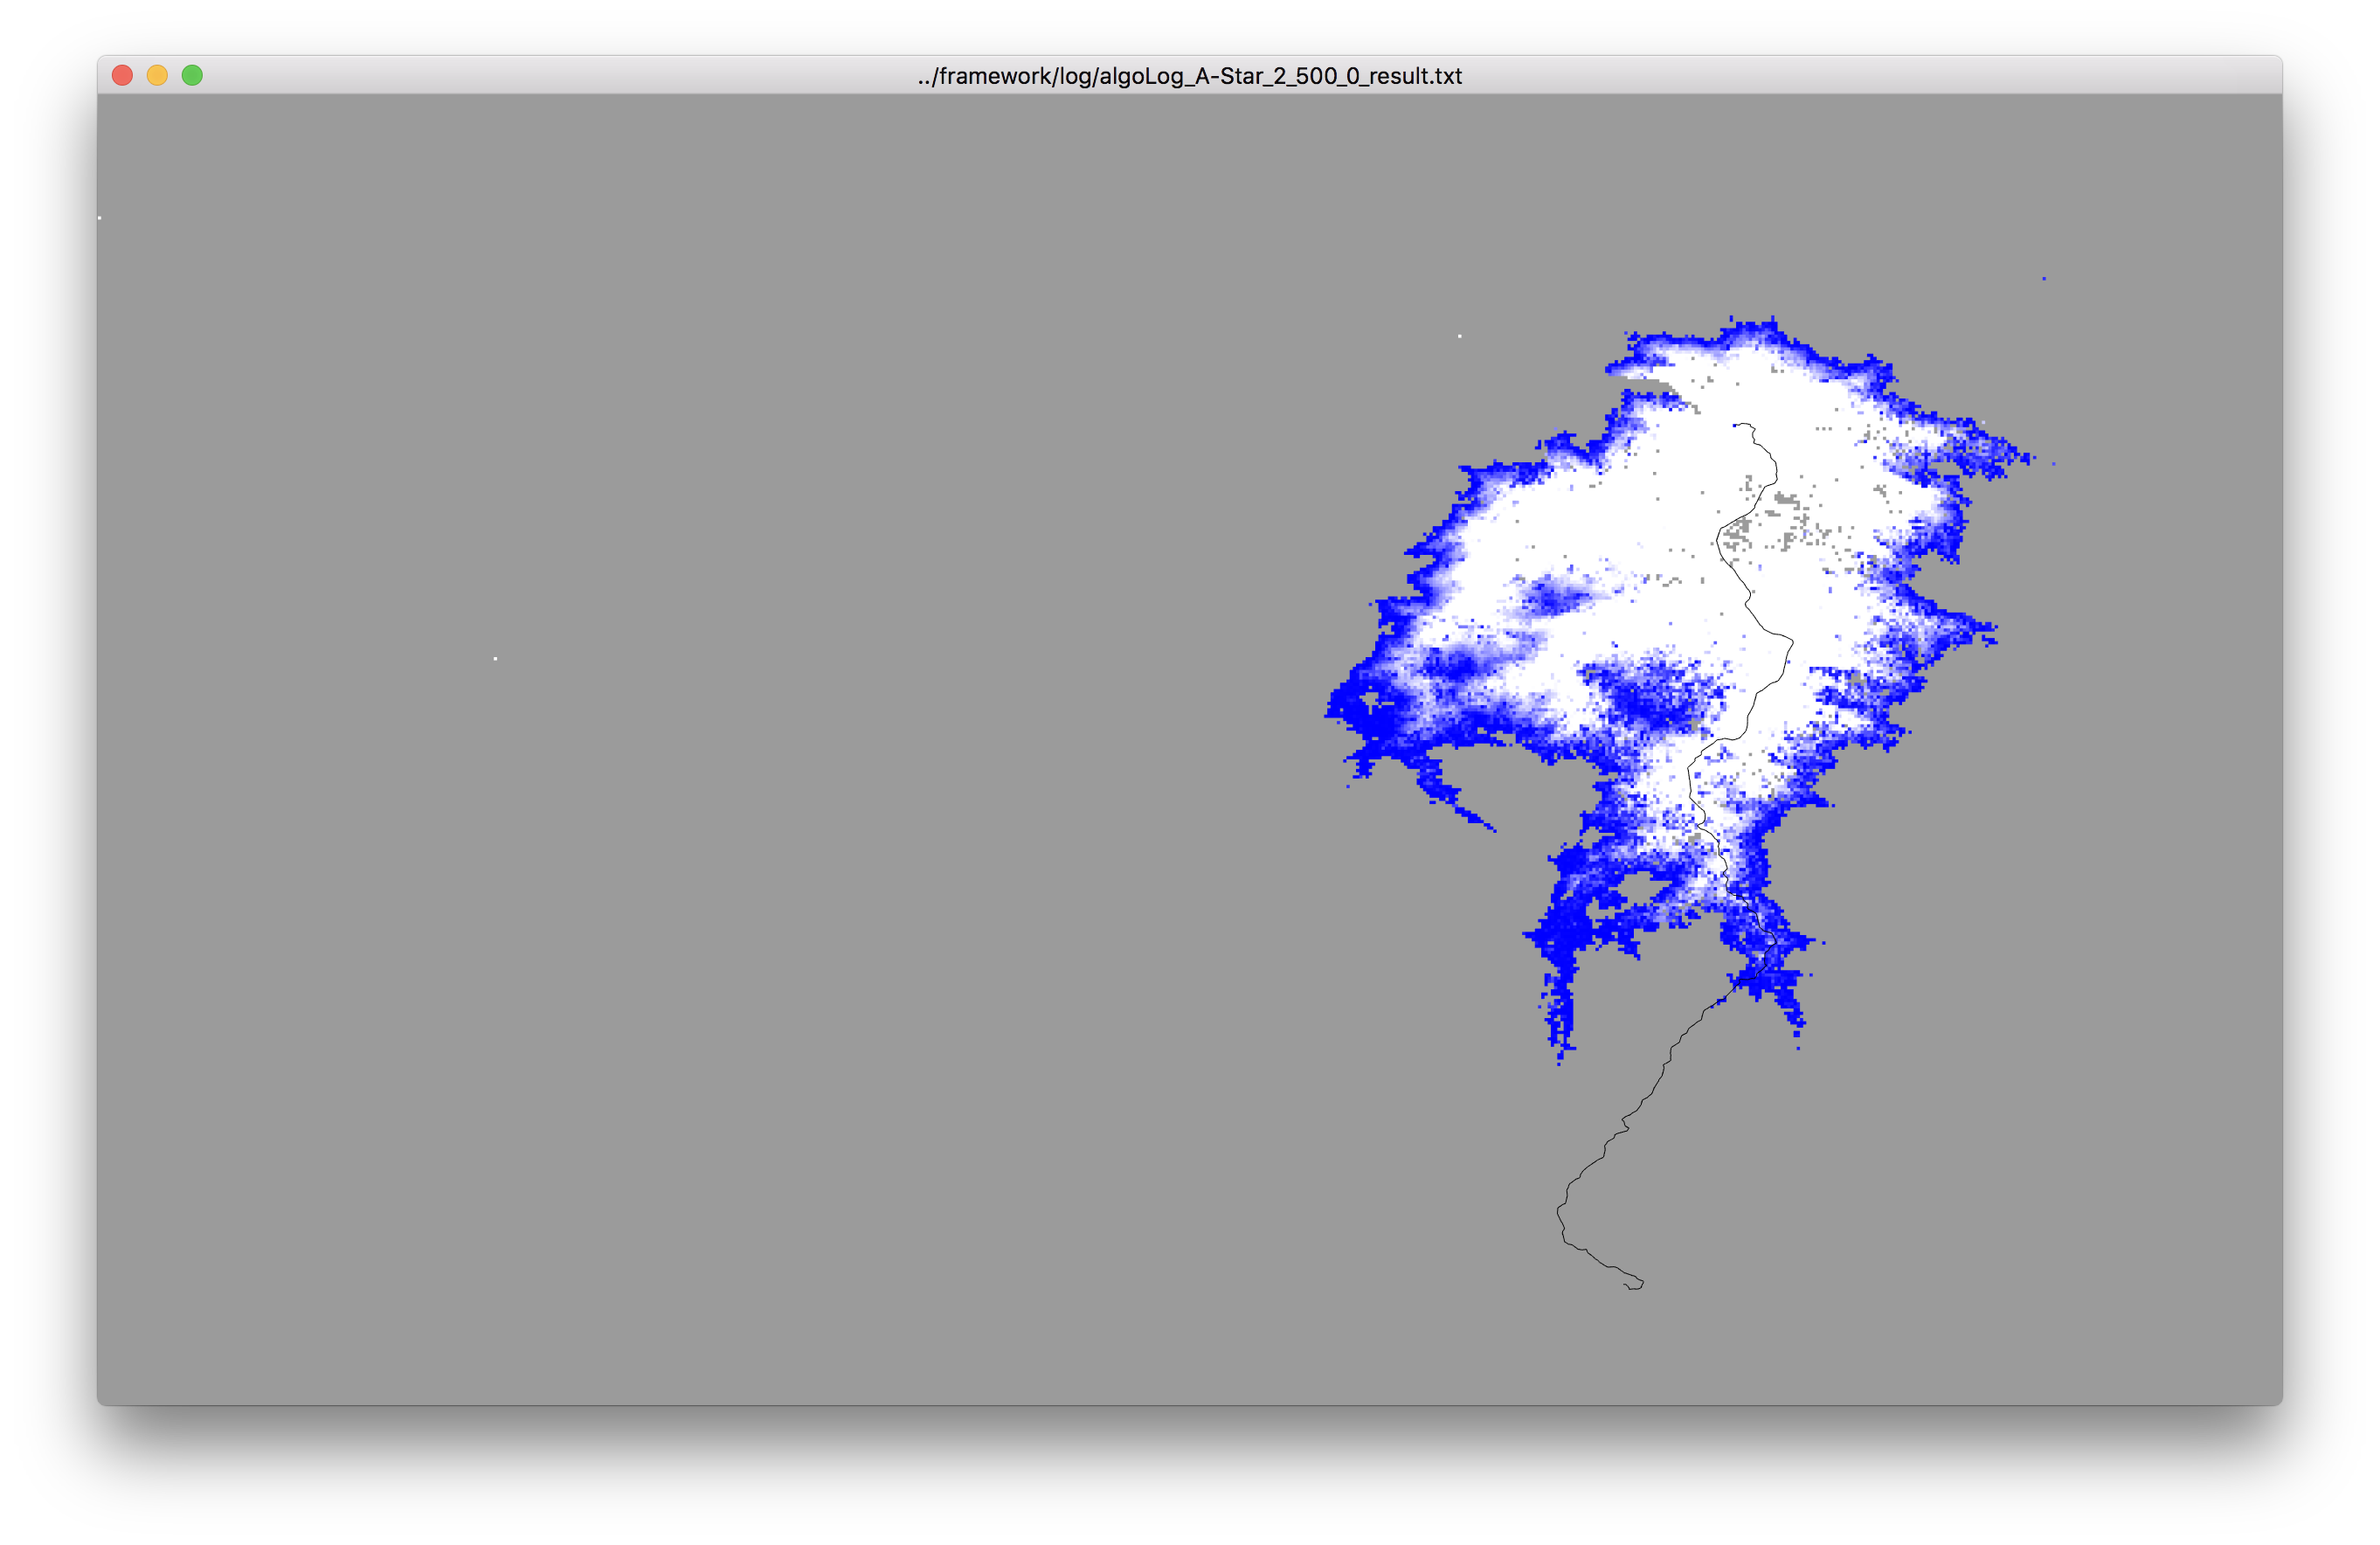
\includegraphics[width=\textwidth]{Images/vis-aged-coloring.png}
\caption[]{Age based coloring. Newly loaded tiles are colored blue and get brighter the longer they have not been loaded. The searched path is represented in green.}
\label{fig:color_aged_tile}
\end{figure}

In \Cref{fig:color_aged_tile} we see that this approach leads to a much better understanding of the sequence of tile-loads.
Thereby it adds a lot of comprehensibility on how the algorithm performs on the underlying graph.

In the specific case displayed in \Cref{fig:color_aged_tile} for example, we can see that most of the recently loaded tiles are located on the outside of the explored graph, but there are three bigger parts in the inner graph as well.
After an examination of those areas we found a simple explanation.
The bigger recently processed tiles are located between freeways.
Therefore the algorithm was observing the freeways first and then slowly spreading from the freeway exits.

\paragraph{Showing the Correct Region of the Graph}
In this paragraph, we are going to explain something we took for granted previously in this chapter.
Somehow, we have to decide where we want to place the elements in the visualization.
We want to show the same element at exactly the same spot in the whole visualization.
Therefore the visualization needs to consider which region of the graph it wants to show before it displays the first element.
As the displayed graph grows as the algorithm progresses there is the risk of growing out of the screen when we estimate the final graph too small.
On the other side, a graph that is estimated to big, which would result in much unused space on out screen.

We considered multiple approaches to solve this issue.
Firstly we developed an estimation method, that estimates the extent of the explored graph of the fully evolved algorithm.
For estimating, this method uses the linear distance between start and target node as the basis.
Because we need to make sure, that the visualization shows everything that is going to happen during the algorithm, it uses a little more than the distance between start and target node as the radius of a circle around the start node.
This circle then flushs with the borders of the visualization, as we assume that the final graph is going to fill this circle.

\begin{figure}
    \fbox{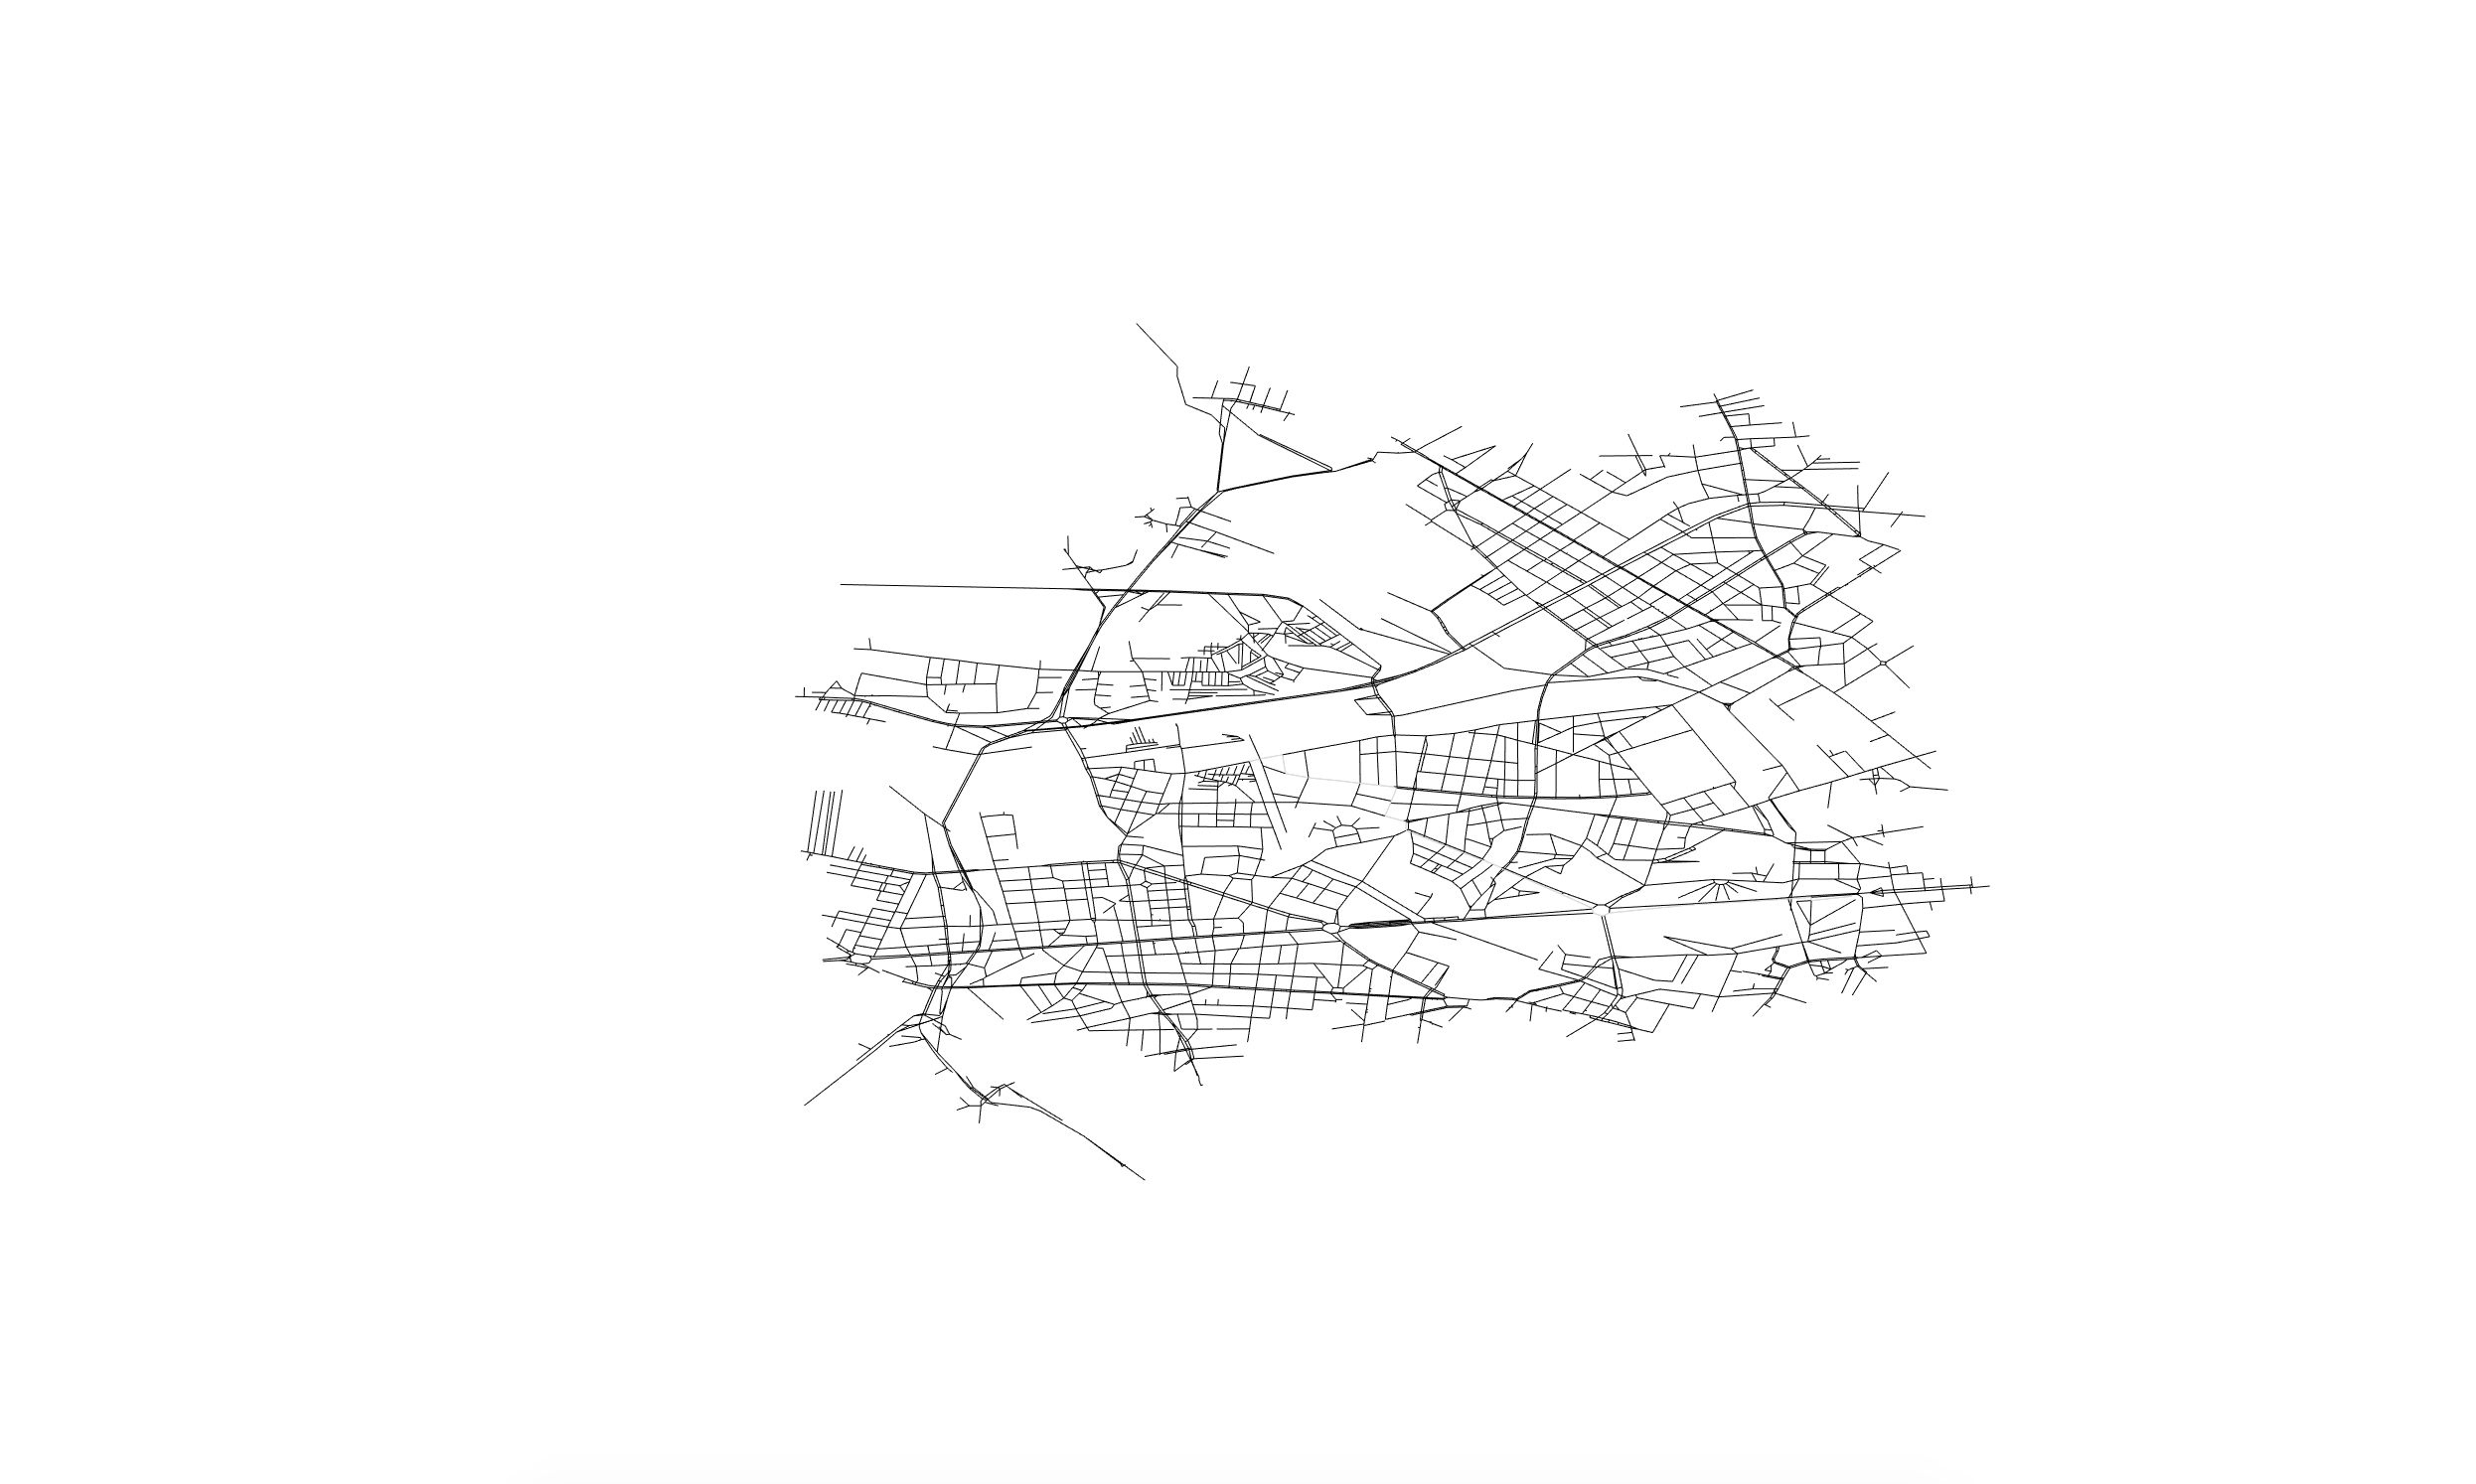
\includegraphics[width=\textwidth]{Images/vis-estimation.png}}
\caption[]{Final state of the visualization, using the Estimation method on the edge-based visualization.}
\label{fig:estimation}
\end{figure}

In \Cref{fig:estimation} we can see that we have got quite a lot unused space using this estimation.
Even though this estimation is quite generous, the actual graph could still grow over the estimated circle.
In general, it is, of course, possible to provide better estimations, but the more precise we would like the estimation to be, the more information we would need about the specific algorithm and the underlying graph, which we want to avoid.

Another method would be to iterate over the algorithm before visualizing it, and therefore find the exact borders of the graph.
With this knowledge, we could then adjust the shown section to exactly fit the fully evolved graph.

\begin{figure}
    \fbox{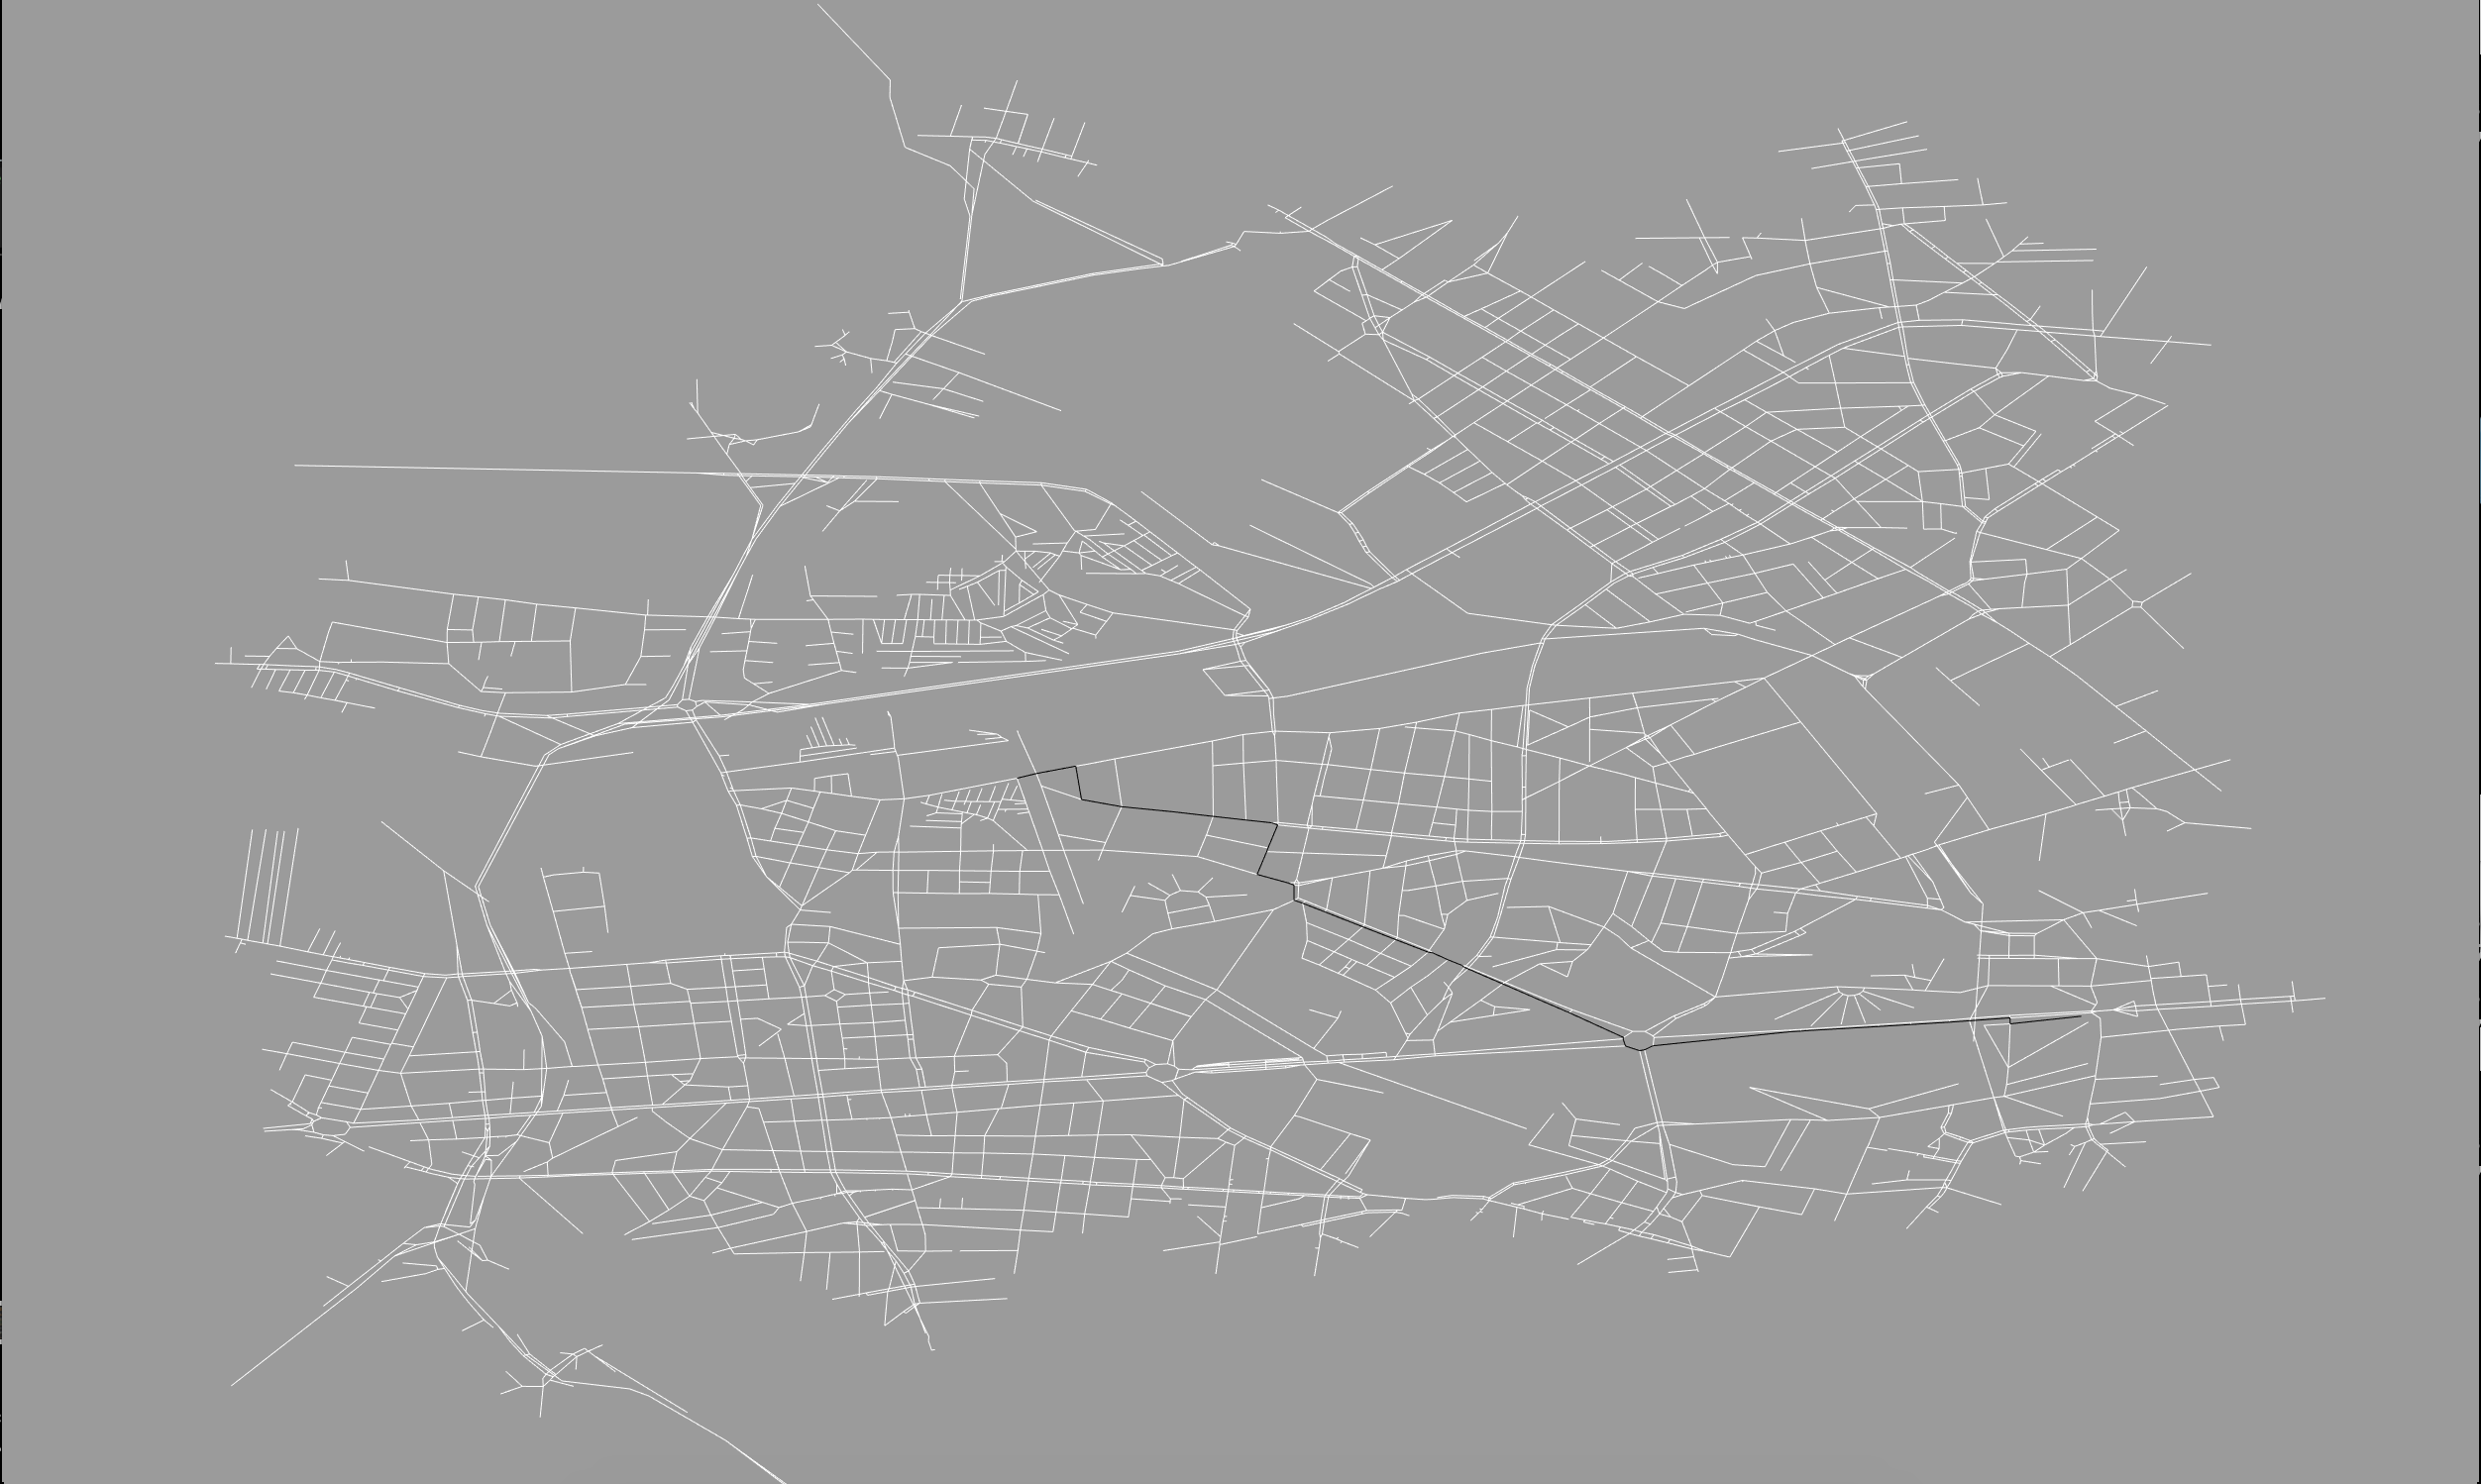
\includegraphics[width=\textwidth]{Images/vis-preprocessing.png}}
\caption[]{Final state of the visualization, using the Preprocessing method on the edge-based visualization.}
\label{fig:preprocessing}
\end{figure}

\Cref{fig:preprocessing} shows a visualization that uses the entire available space on one axis.
As this method is using the same scale on both axes there could be bigger unused space on the other axis.

Based on this we developed another method, that changes the scale on one of the axes to fit the window of the visualization as well.
Thereby it spreads the graph over the whole screen.

\begin{figure}
    \fbox{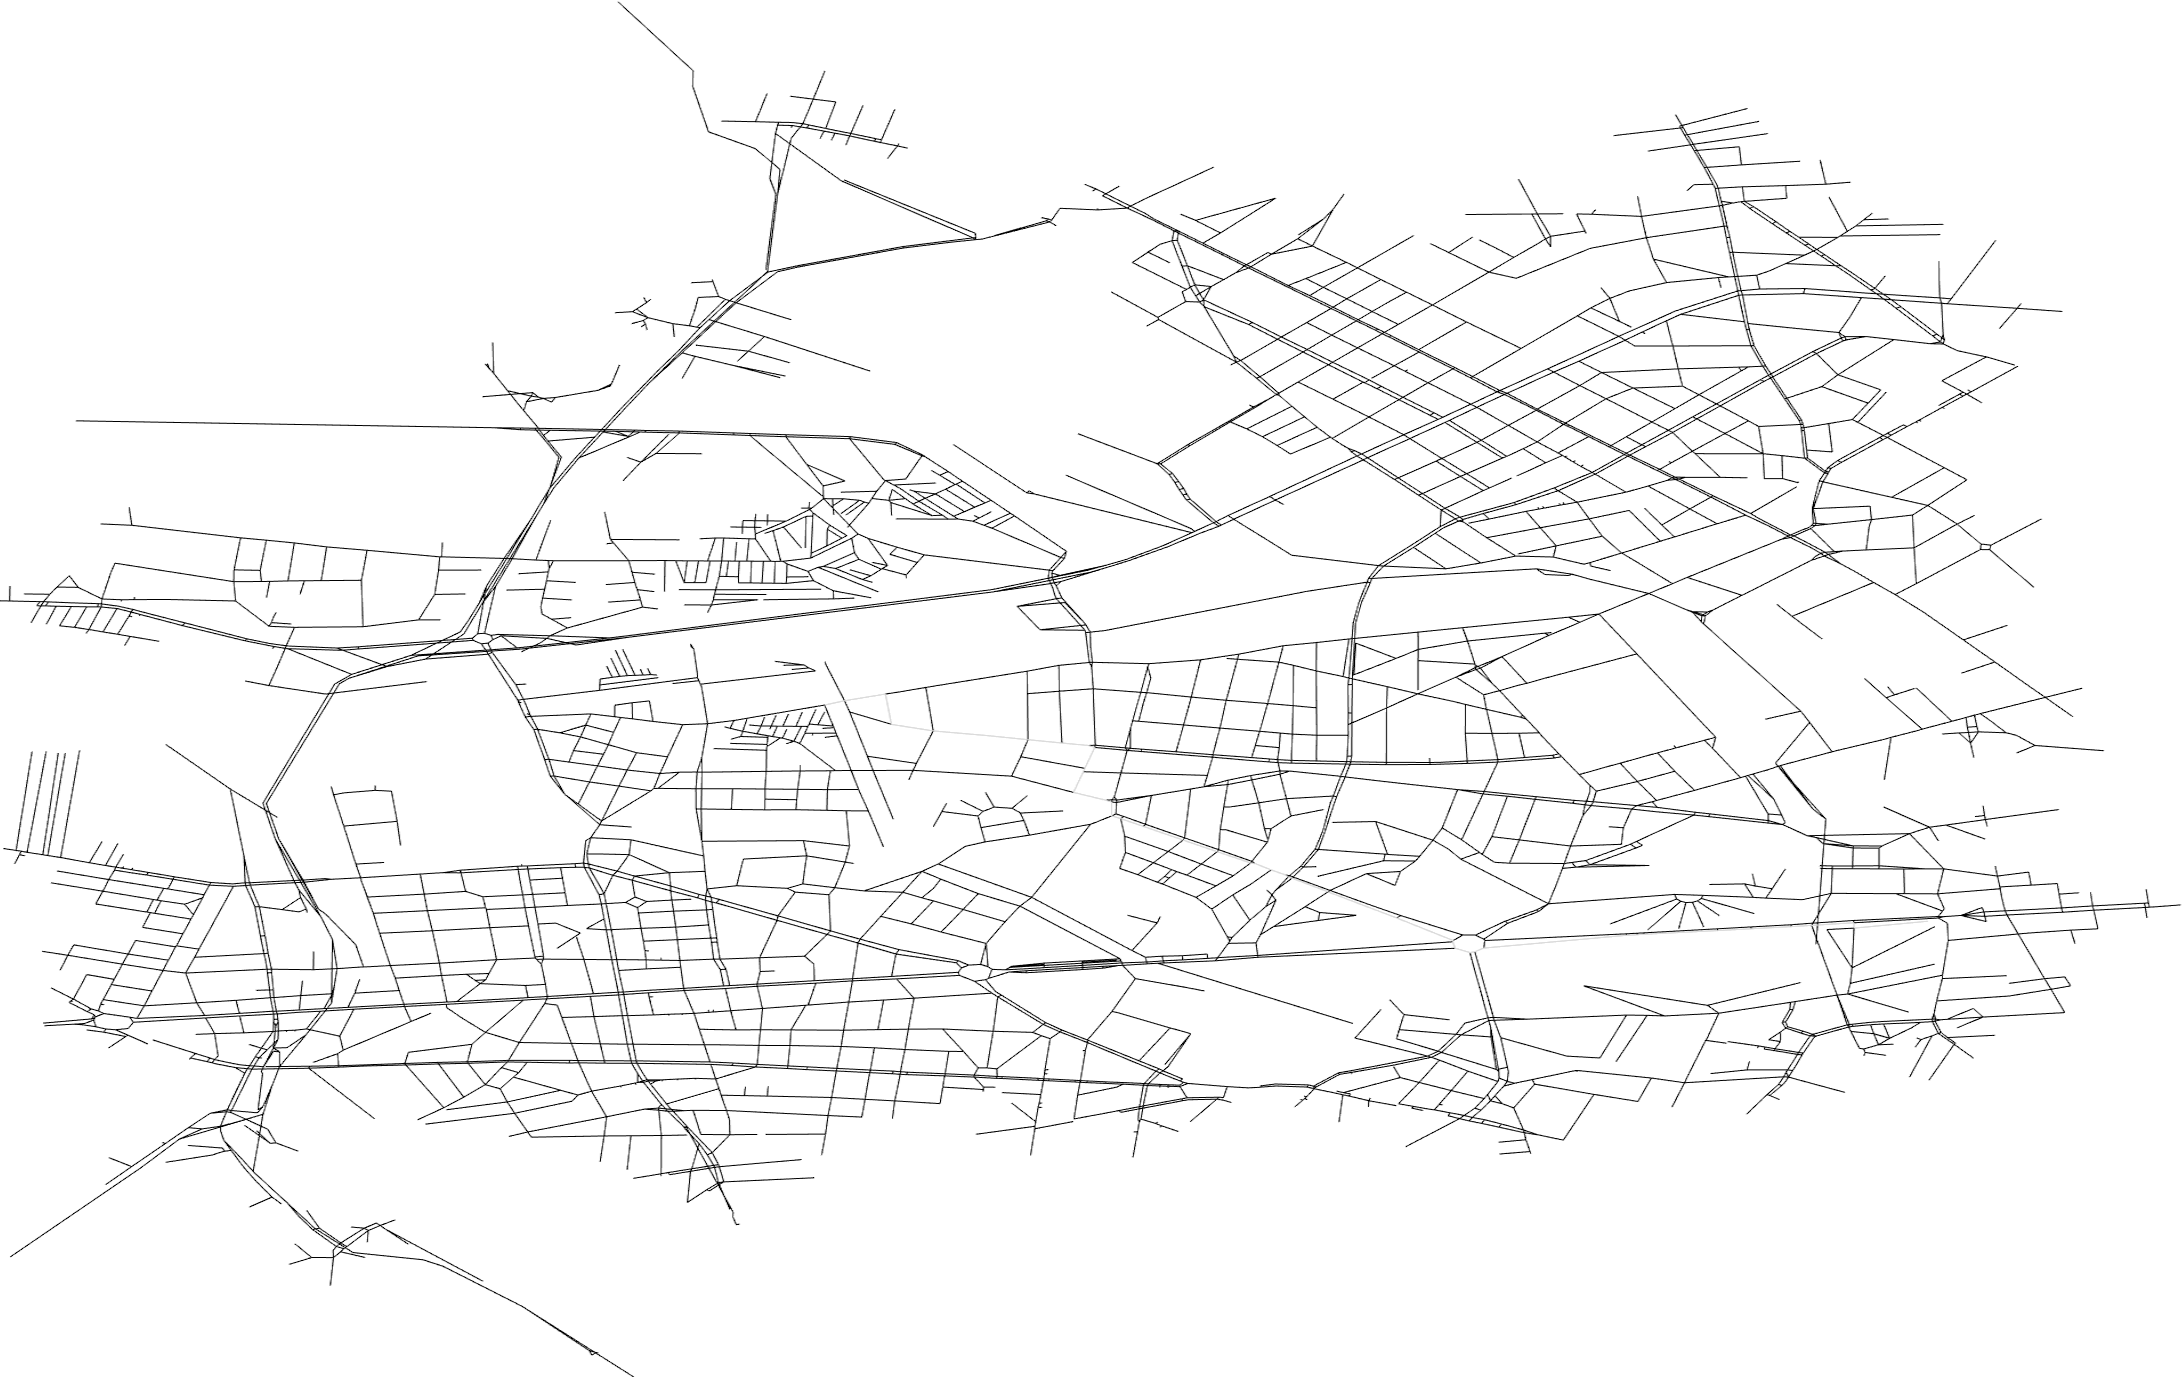
\includegraphics[width=\textwidth]{Images/vis-preprocessing-streched.png}}
\caption[]{Final state of the visualization, using the Preprocessing method with additional streching to the borders of the visualization on the edge-based visualization.}
\label{fig:spreaded_axis}
\end{figure}

As we see in \Cref{fig:spreaded_axis} this reduces the unused space to a minimum.
Though we loose a lot of understandability, as the length of a line on the screen would indicate the length of the real edge even less.

As a result, we decided to use the preprocessing method with uniform axes for our visualization.
On the one hand, the additional performance costs in preprocessing are worth the reduced amount of unused space.
On the other hand, the possible unused space on one axis is worth the increased comprehensibility.


\subsection{Visualizing the Cache} \label{cache}

In this section, we explain a way to display the cache in the visualization.
Taking the tiles as a foundation, we represent the cache by coloring the contained tiles.

\begin{figure}
    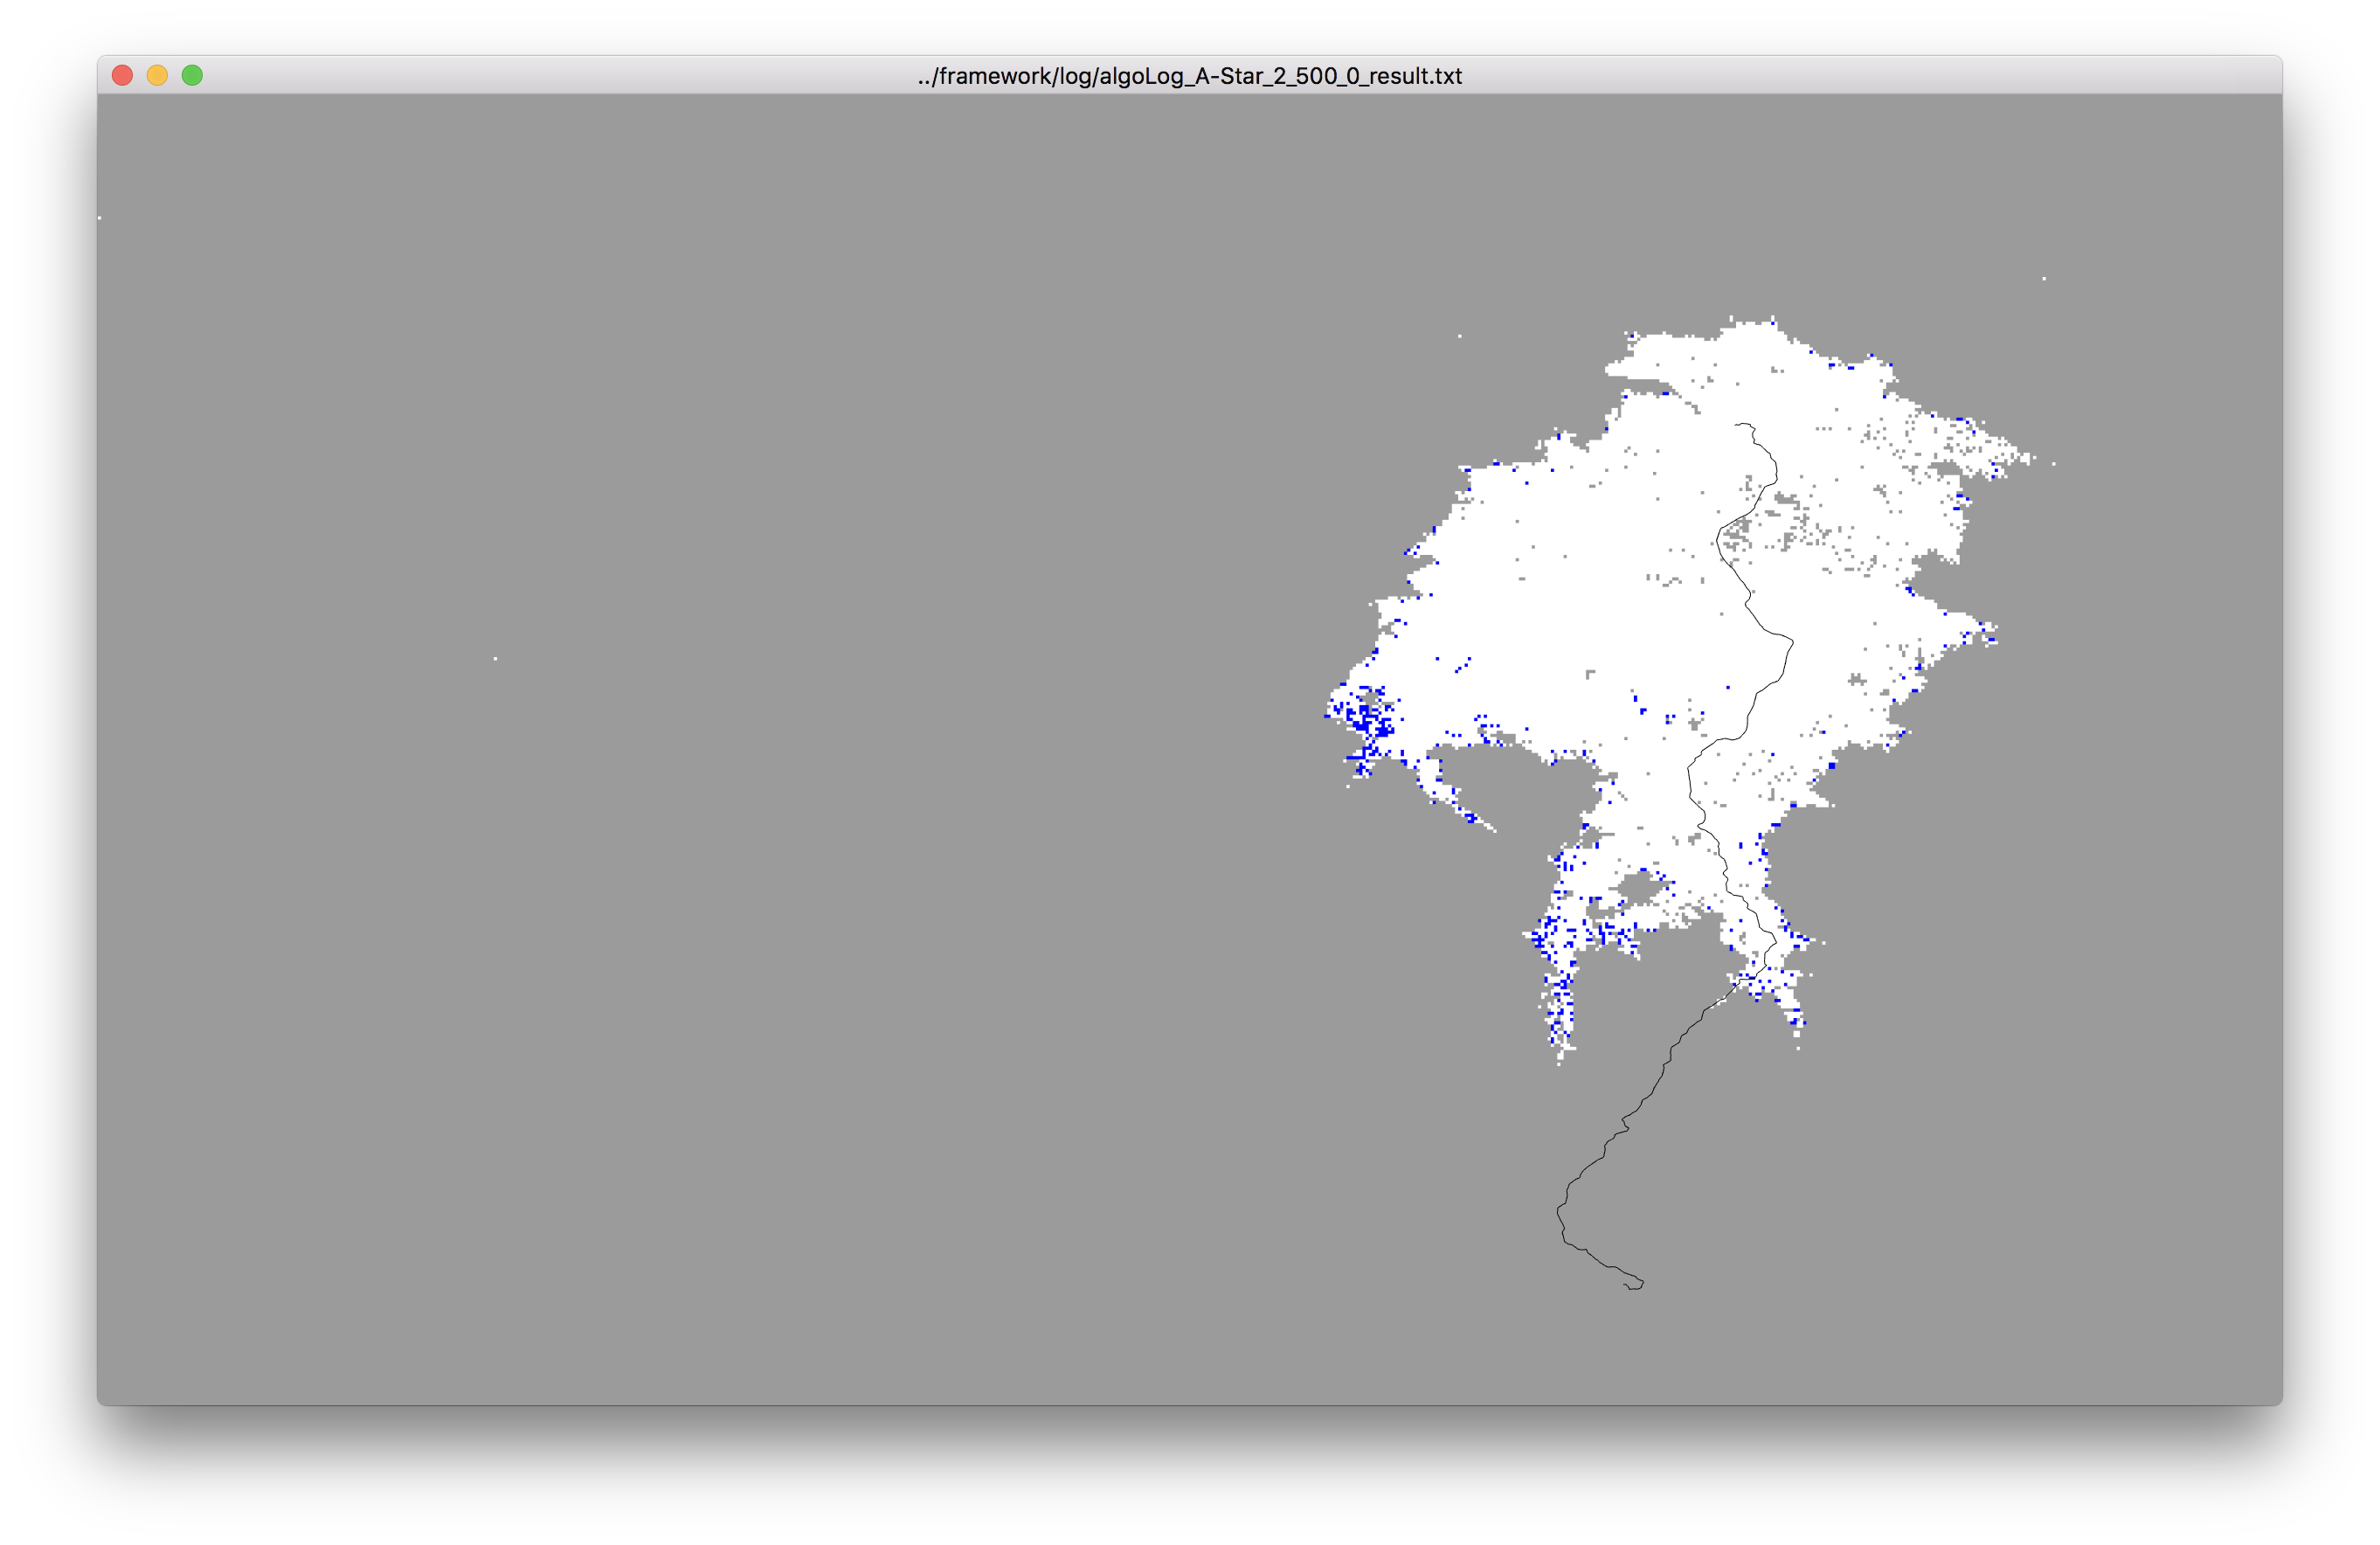
\includegraphics[width=\textwidth]{Images/vis-basic-cache.png}
\caption[]{Representing the cache. The cache is represented by the blue rectangular shapes. The searched path is represented in green.}
\label{fig:cache_coloring}
\end{figure}

In \Cref{fig:cache_coloring} we can see, that we did not color the tiles based on their age anymore.
Due to the colored cache, we achieved an improved understanding of past loaded tiles and the aged based coloring would furthermore distract from the important cache.

For showing how well an algorithm performs, we color every tile, whenever it is not in the cache according to the frequency it has been loaded.

\begin{figure}
    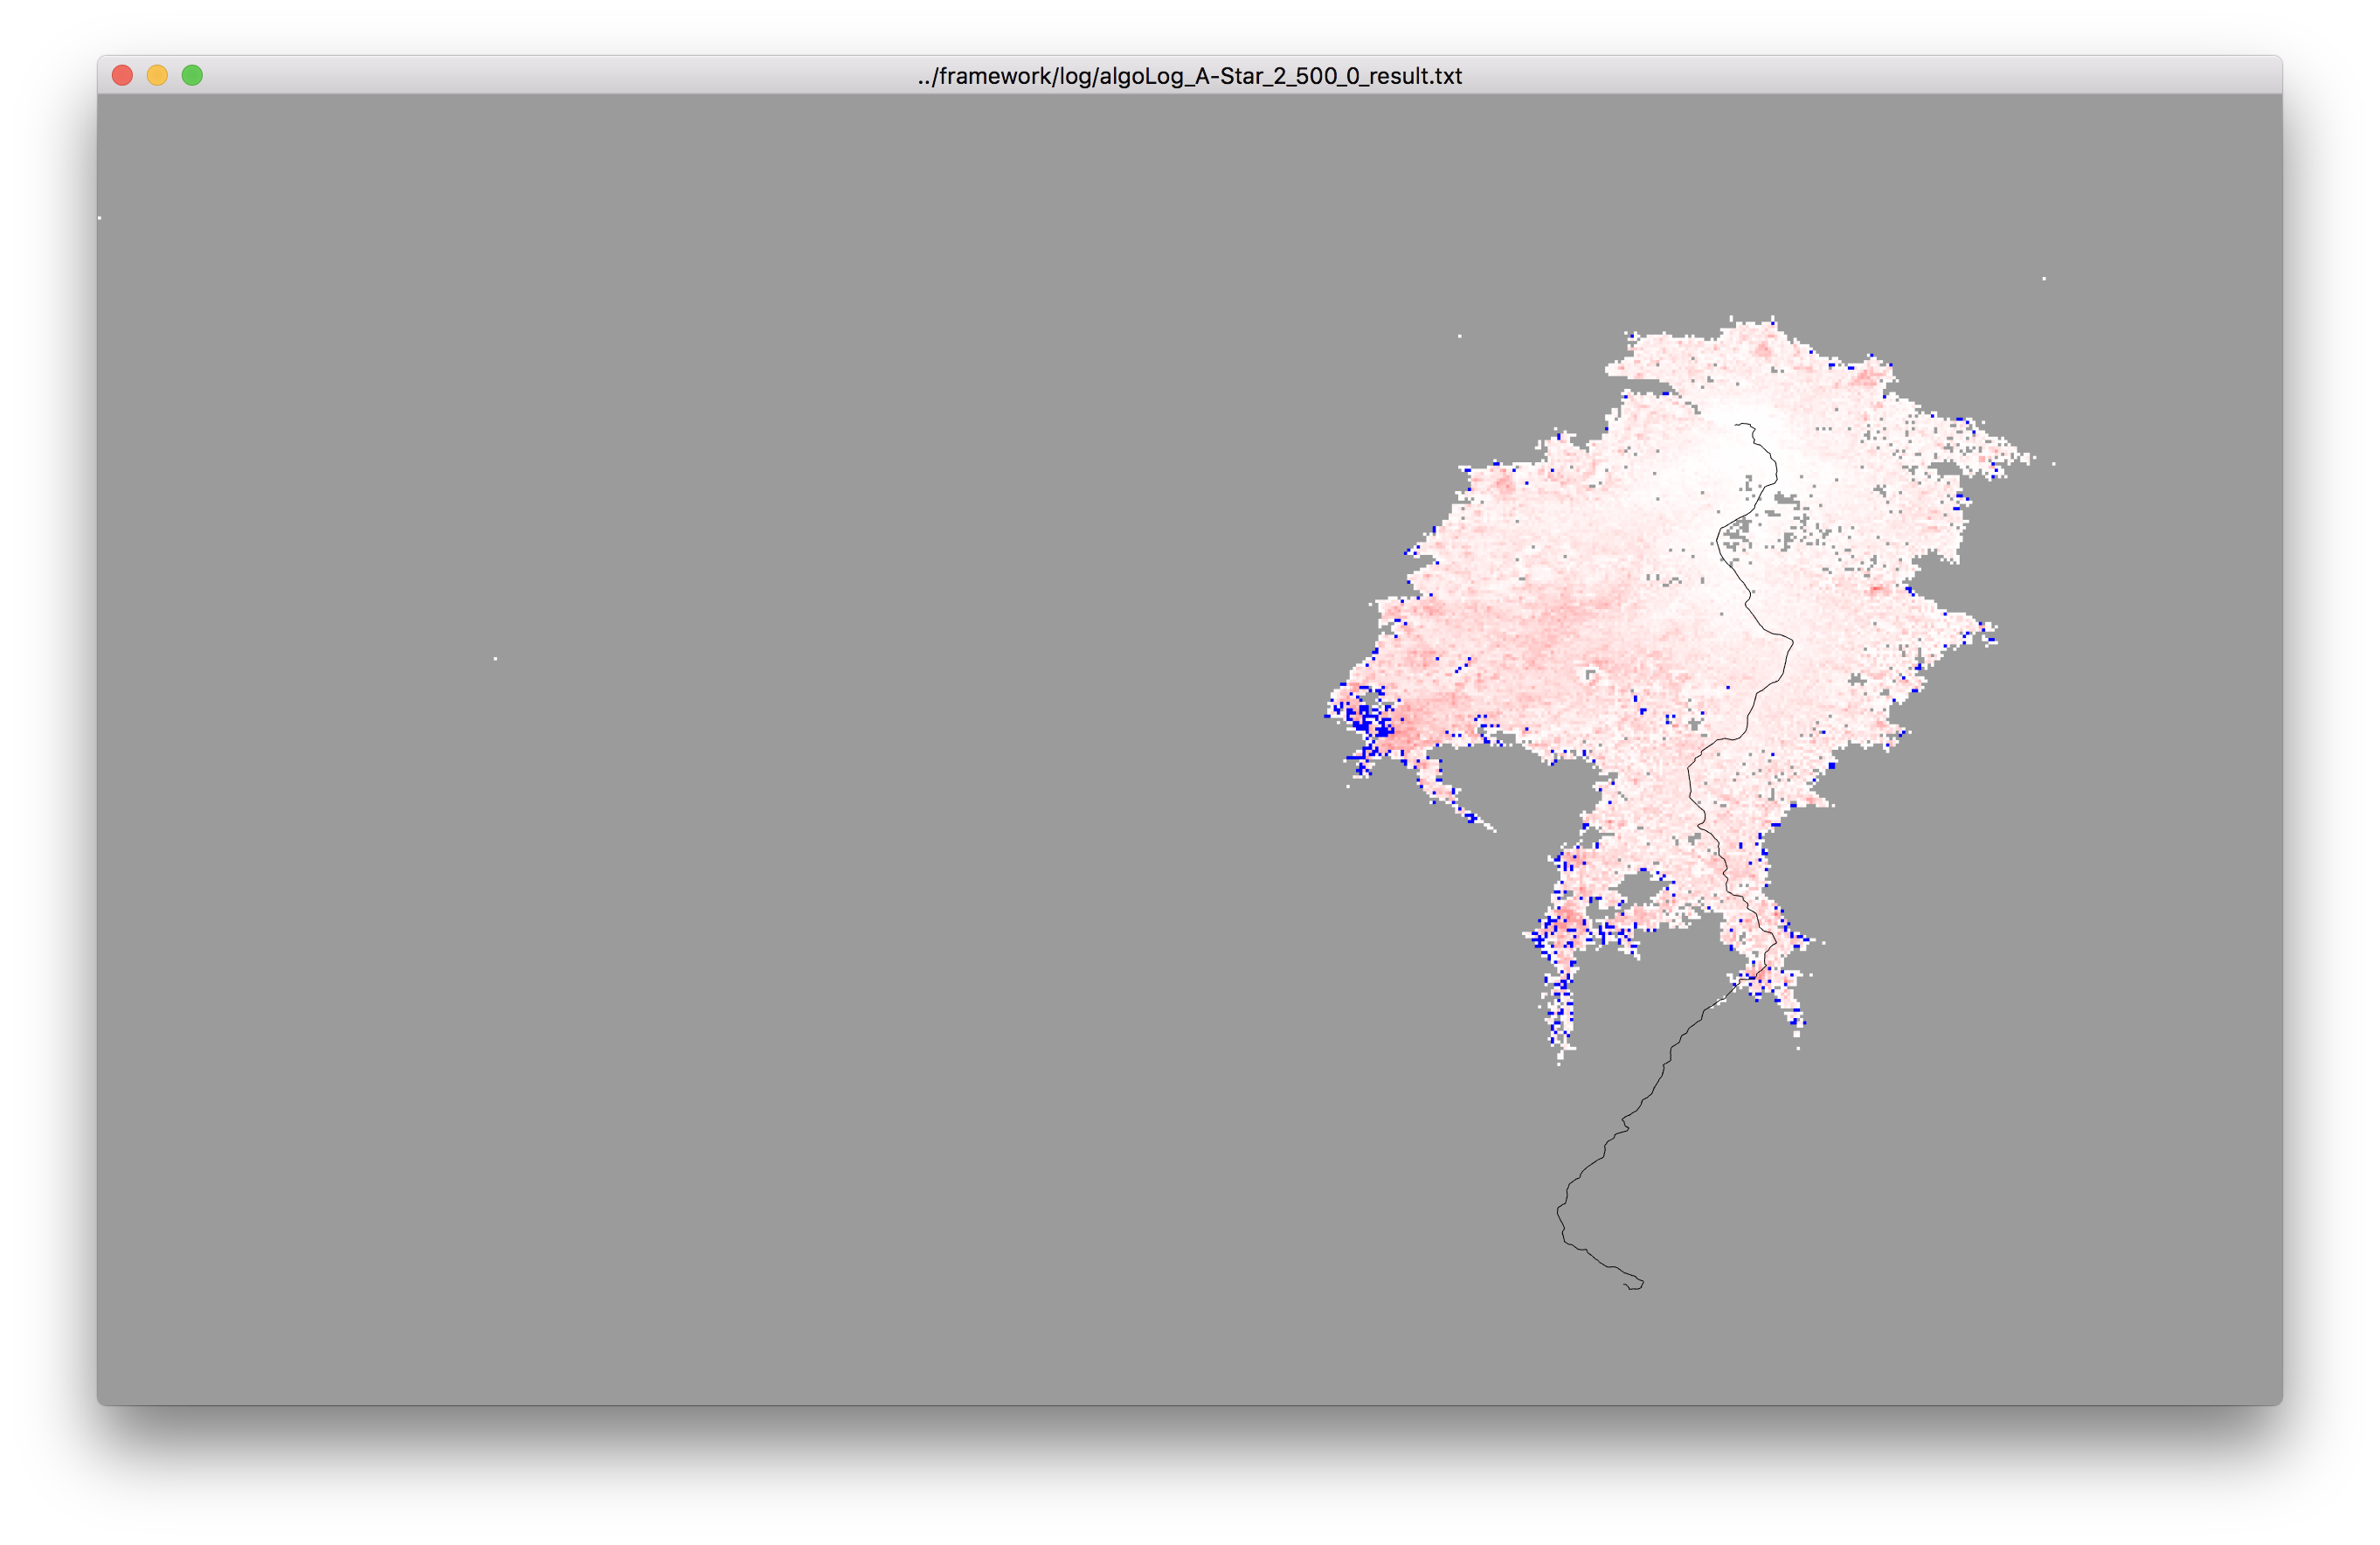
\includegraphics[width=\textwidth]{Images/vis-rgb-cache.png}
\caption[]{Coloring the tiles according to the amount of reloads. Red tiles has been loaded more often. The searched path is represented in green.}
\label{fig:reload_coloring_white}
\end{figure}

By coloring the reloads this way, we can now see how good our algorithm performs and in which regions more reloads occur.
With this color scheme, bigger differences in tile loading can be distinguished from each other easily.
Nevertheless smaller differences are hard to recognize.
Therefore, we tried another color scale.


By using a transition between two colors we hope to achieve a bigger and clearer contrast between slightly different tile loads.
The HSV color space enables us to choose any color as a basis and then change the hue linear according to the amount of reloads.

\begin{figure}
    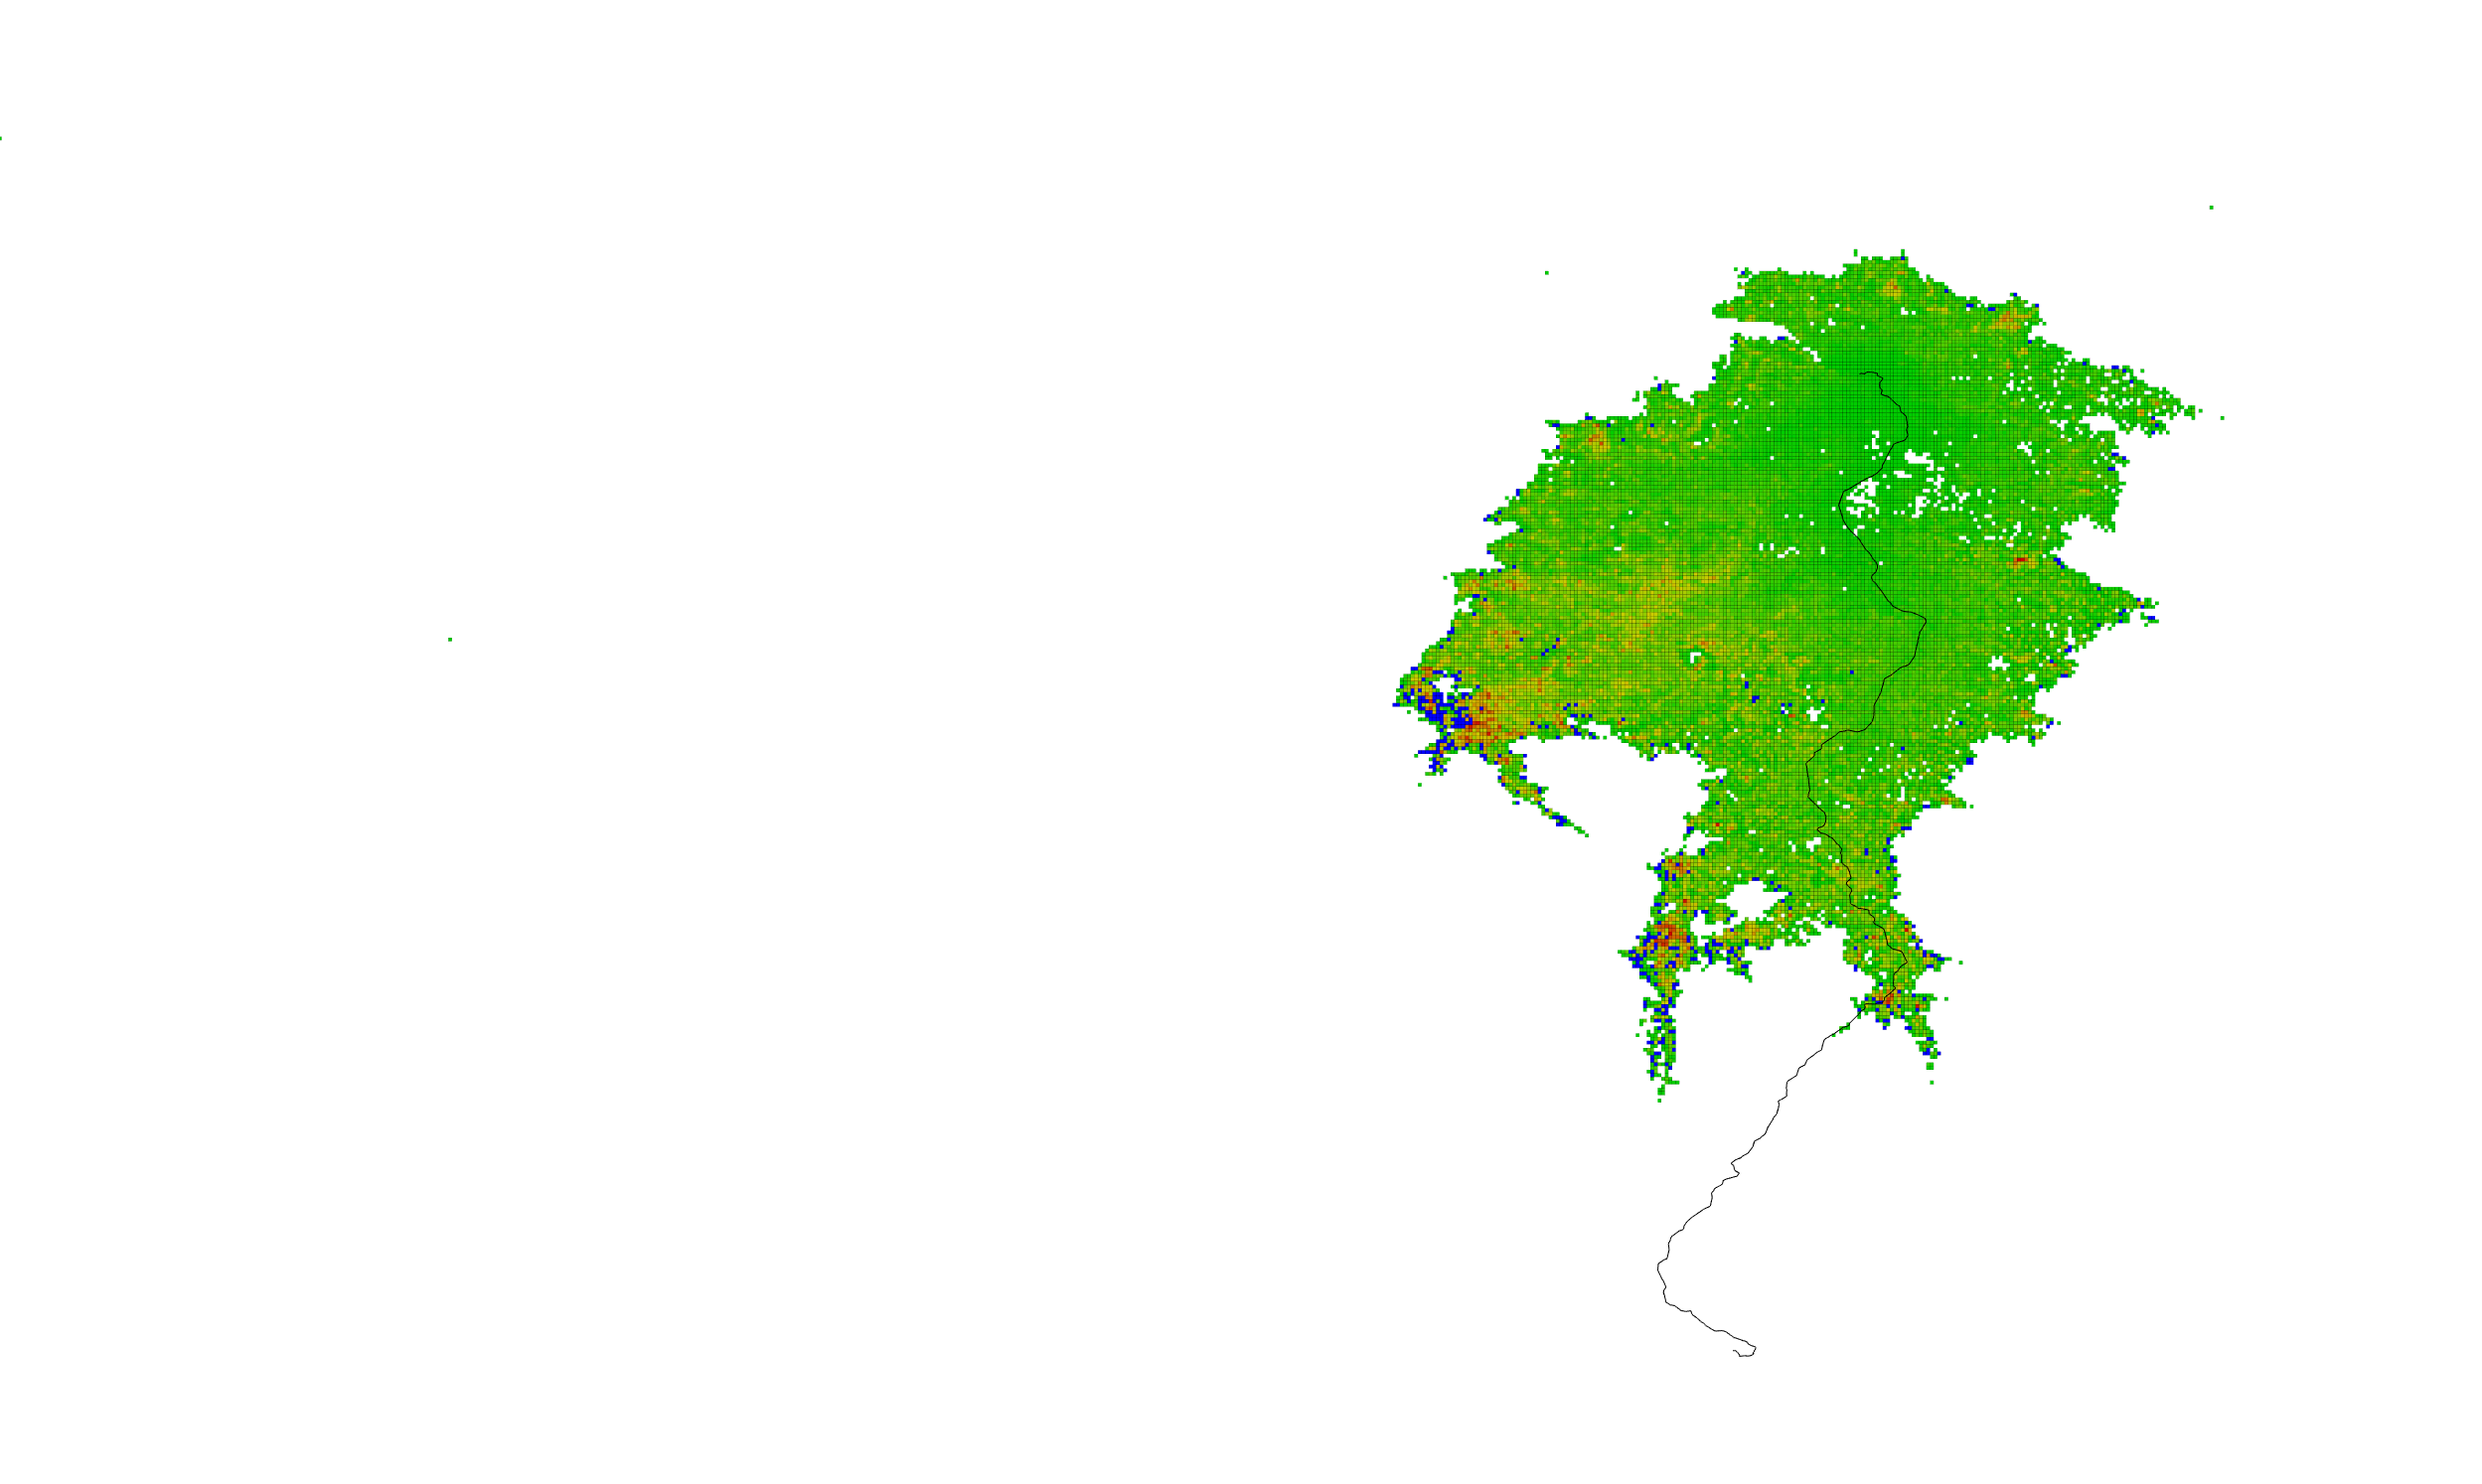
\includegraphics[width=\textwidth]{Images/vis-hsv-cache.png}
\caption[]{Changed color scheme. Now the tiles change their color from green to red. For a better contrast the searched path is now represented in black.}
\label{fig:reload_coloring_hsv}
\end{figure}

In \Cref{fig:reload_coloring_hsv} we see the differences between two similar values clearer than in the transition from an uncolored tile to a specific color.
As a side effect, the graph distinguished from the background much better now and the visualization look much better.

\section{Compare Algorithms} \label{compare}
\todo{altes benutzten vs neues}
A first approach for comparing algortihms is to simply start two visualizations and display them next to each other.

\begin{figure}
    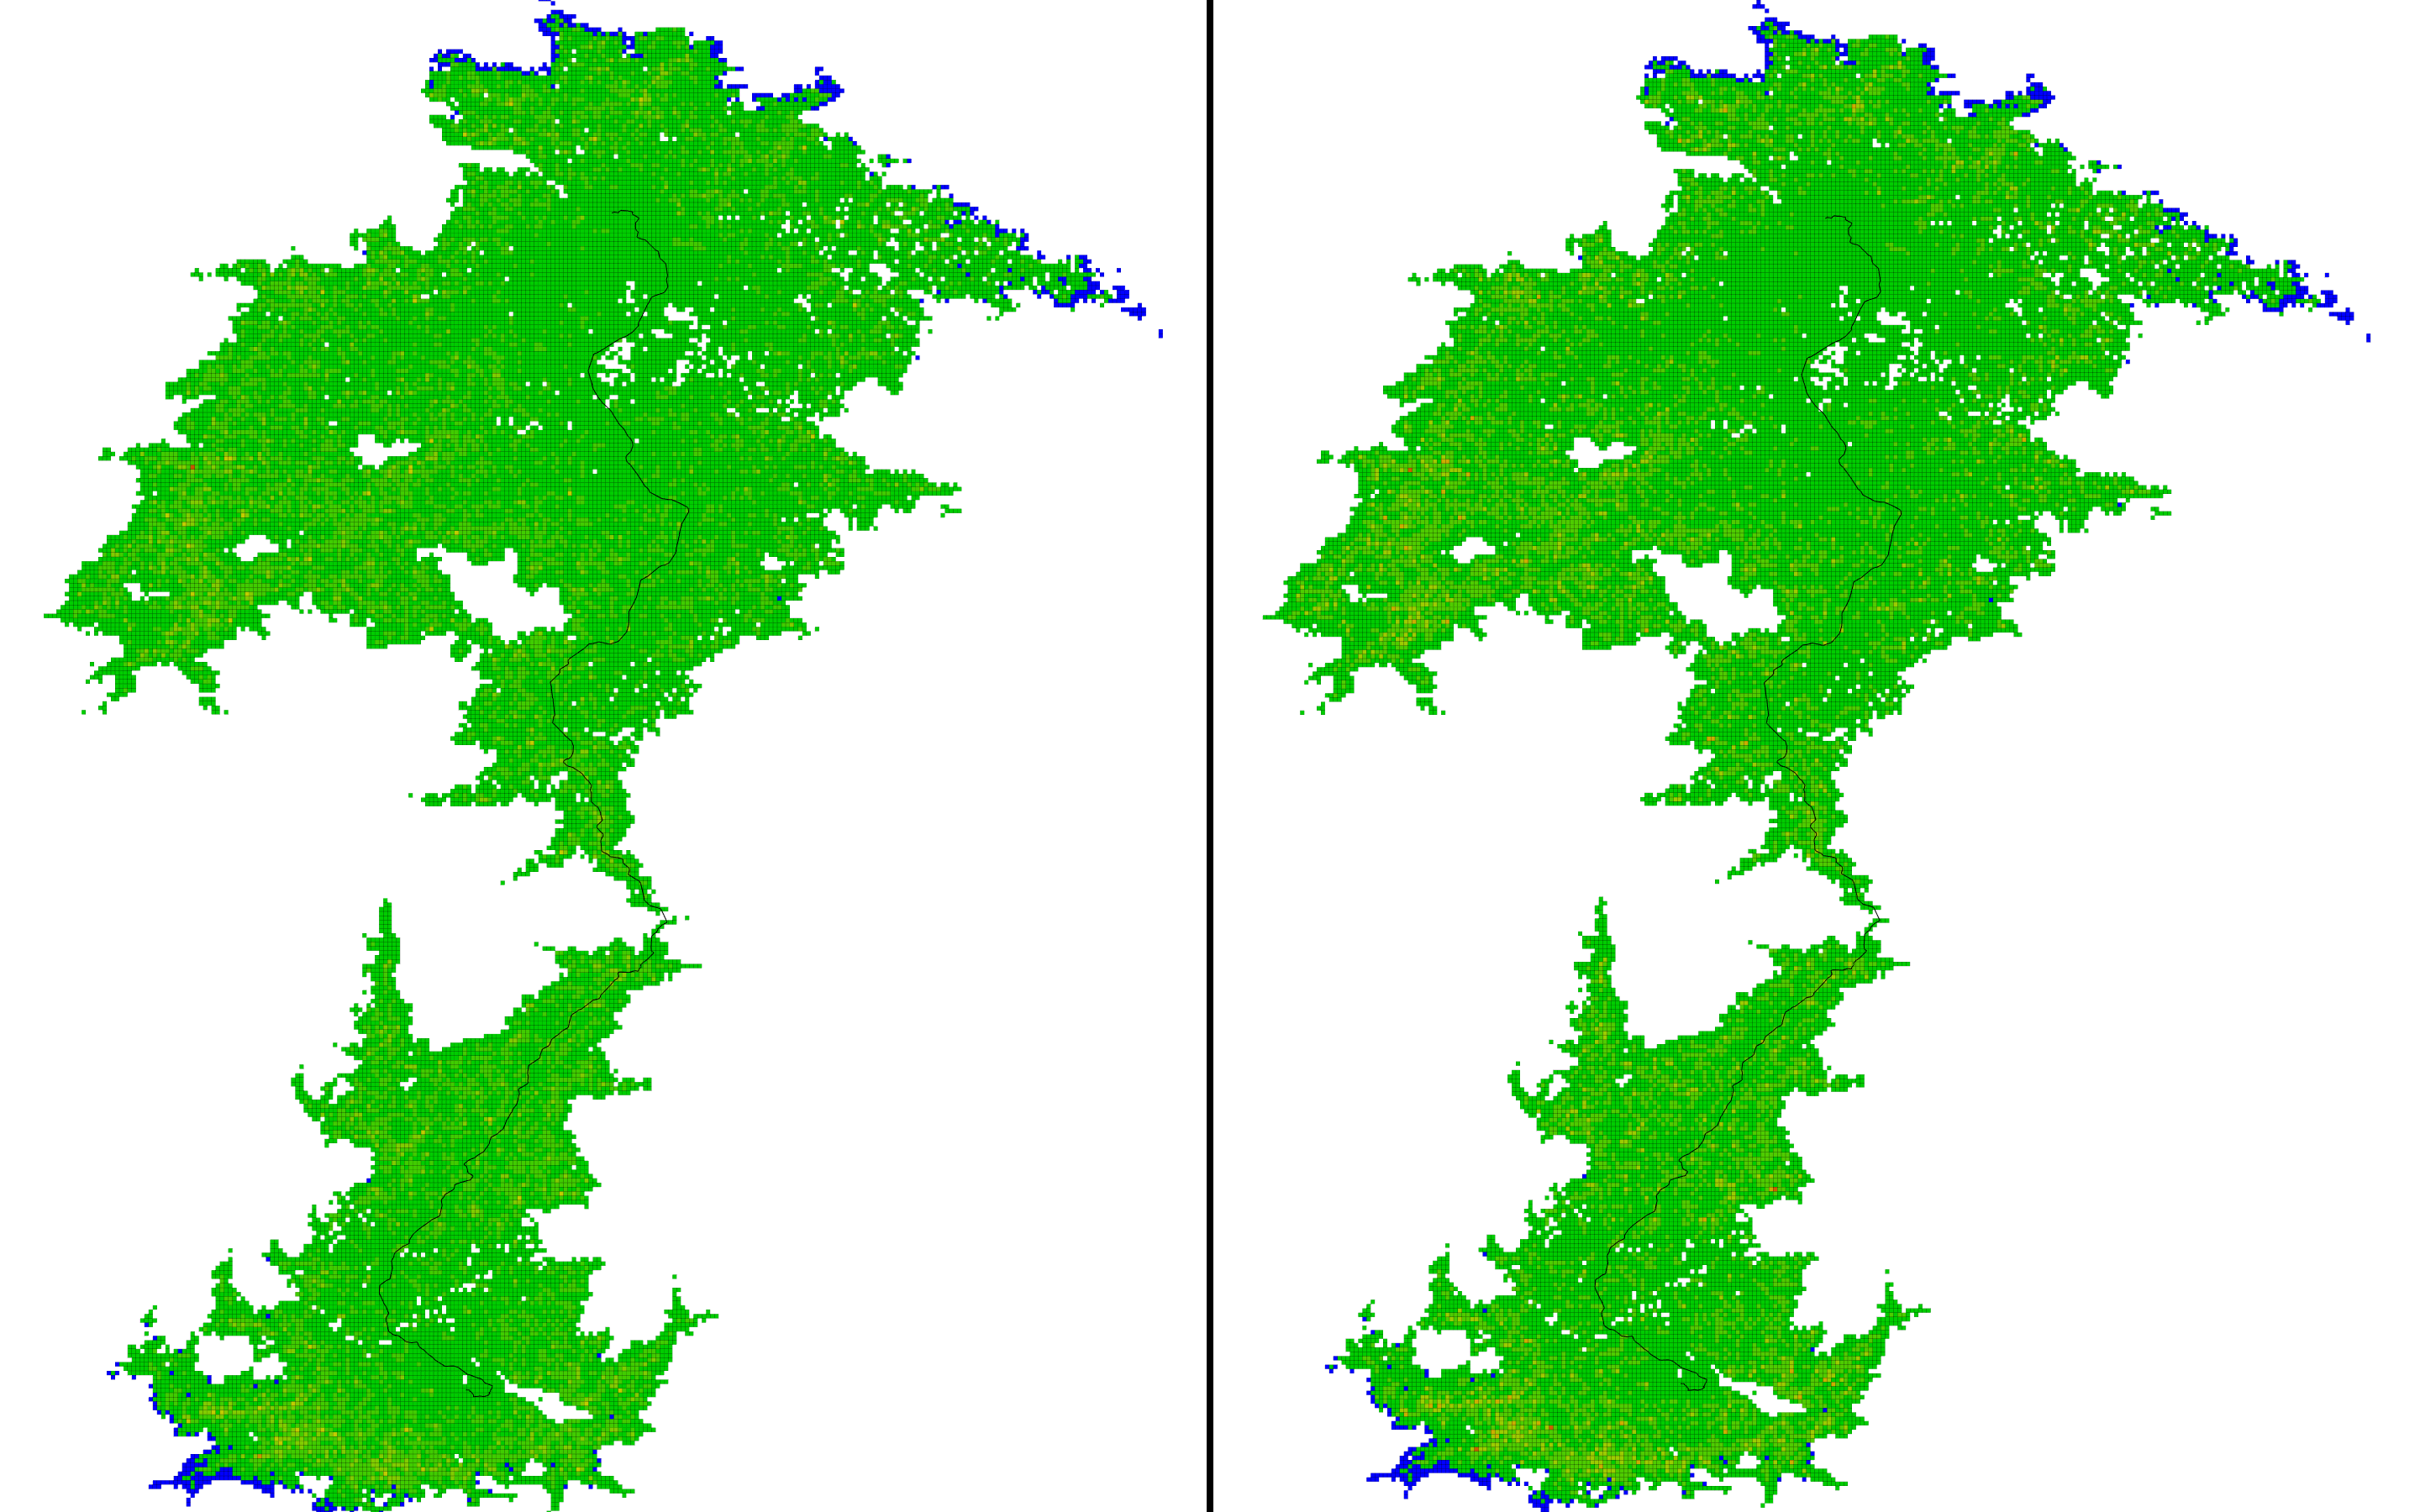
\includegraphics[width=\textwidth]{Images/vis-compare-two.png}
\caption[]{Running two visualizations next to each other.}
\label{fig:two_visualization}
\end{figure}

In \Cref{fig:two_visualization} we can only see smaller difference in the search space of the two algorithms.
We experienced that this kind of comparison is not useful to really examine differences between algorithms, but to show them to others.
For really comparing algorithms we, therefore, needed to develop a new variation of the visualization.
Therefore we removed the space between both visualizations.
The idea is, that smaller differences are better visible when tiles with the same location are displayed directly next to each other.
Therefore we split each tile in two and color the left half according to the reloads of one algorithm and the right half according to the reloads of the other algorithm.

\begin{figure}
    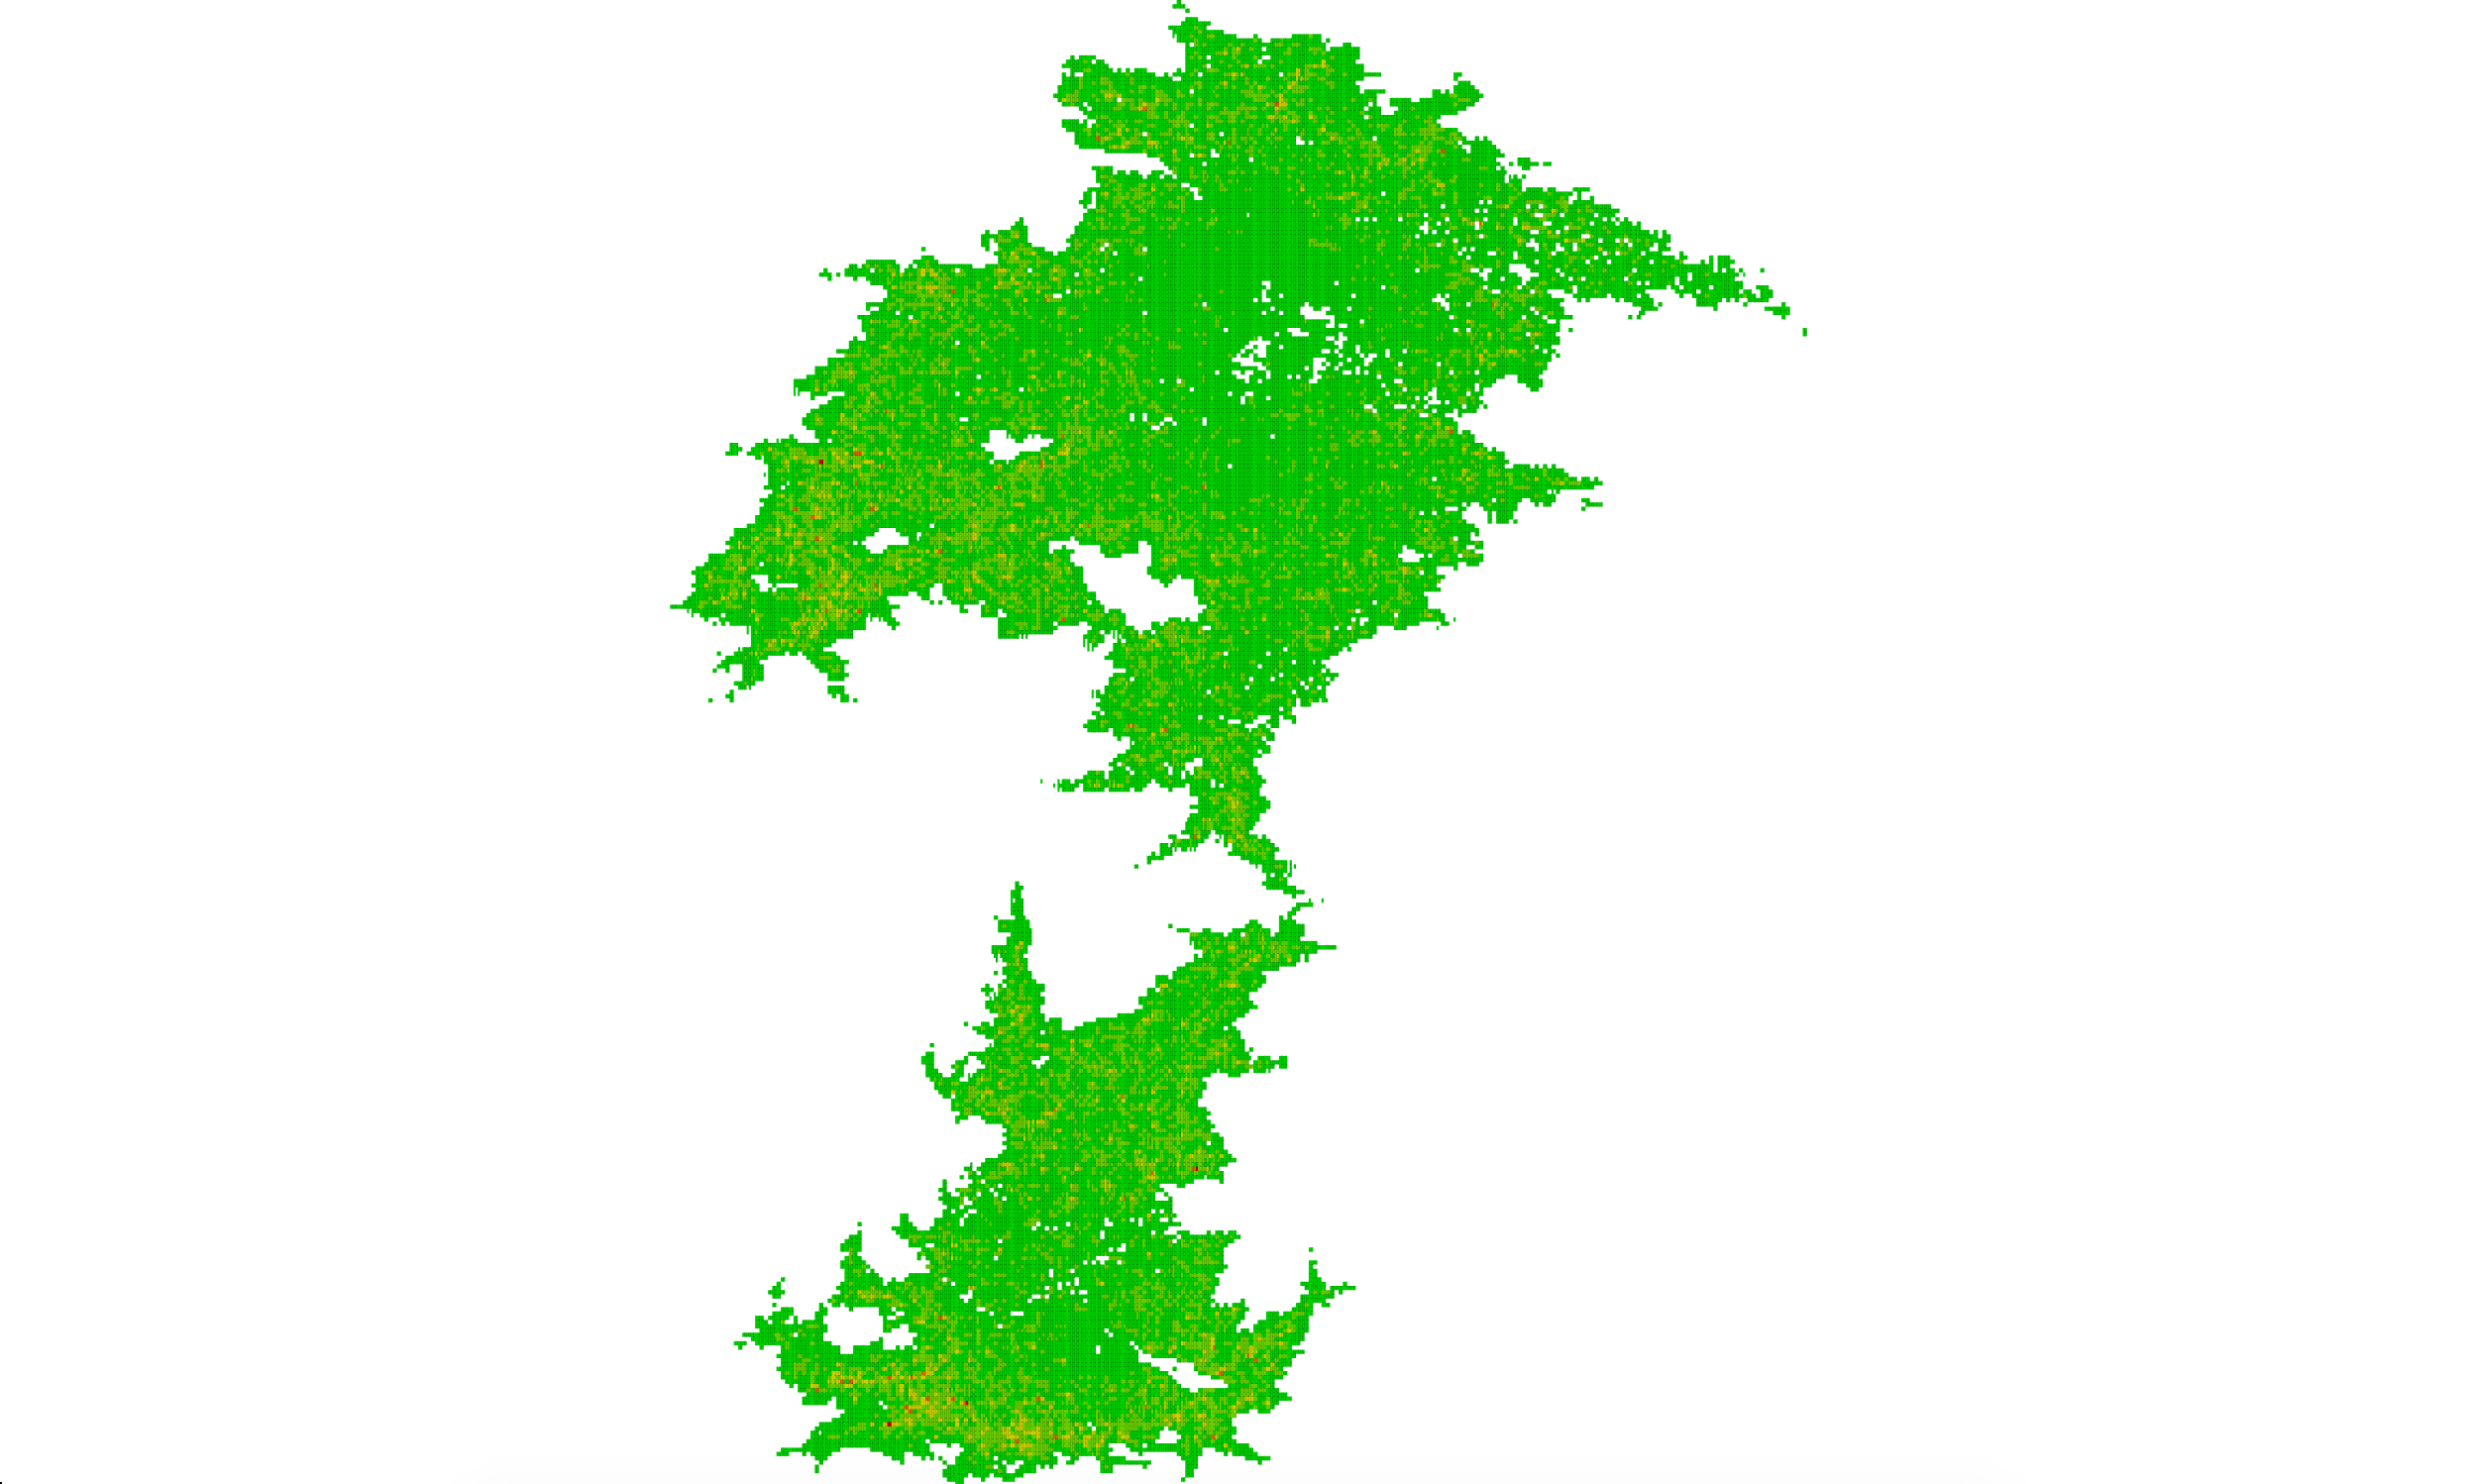
\includegraphics[width=\textwidth]{Images/vis-compare-splitted.png}
\caption[]{Splitting the tiles. The left half of a tile represents one algorithm and the right half the other algorithm.}
\label{fig:splitted_tiles}
\end{figure}

This method provides a better way to see differences on tile level, as we can see in \Cref{fig:splitted_tiles}.
However, it is still difficult to clearly identify the differences without longer observation, as it is hard to associate a tile half to one of the algorithms.
At this point, we could expand this method to label the algorithms with different colored outlines of the tiles, but as we are only interested in the differences between algorithms, when comparing them, we developed an approach that is only showing the difference between the tile loads.

This method calculates the difference between the amount of tile loads from both algorithms for each tile.
Then it displays all the tiles that have been accessed by at least one algorithm and colors those blue that have been loaded more often by the first algorithm.
Those that have been loaded more often by the second algorithm are colored red.
The more intense the color, the bigger is the difference in the amount of tile loads.

\begin{figure}
    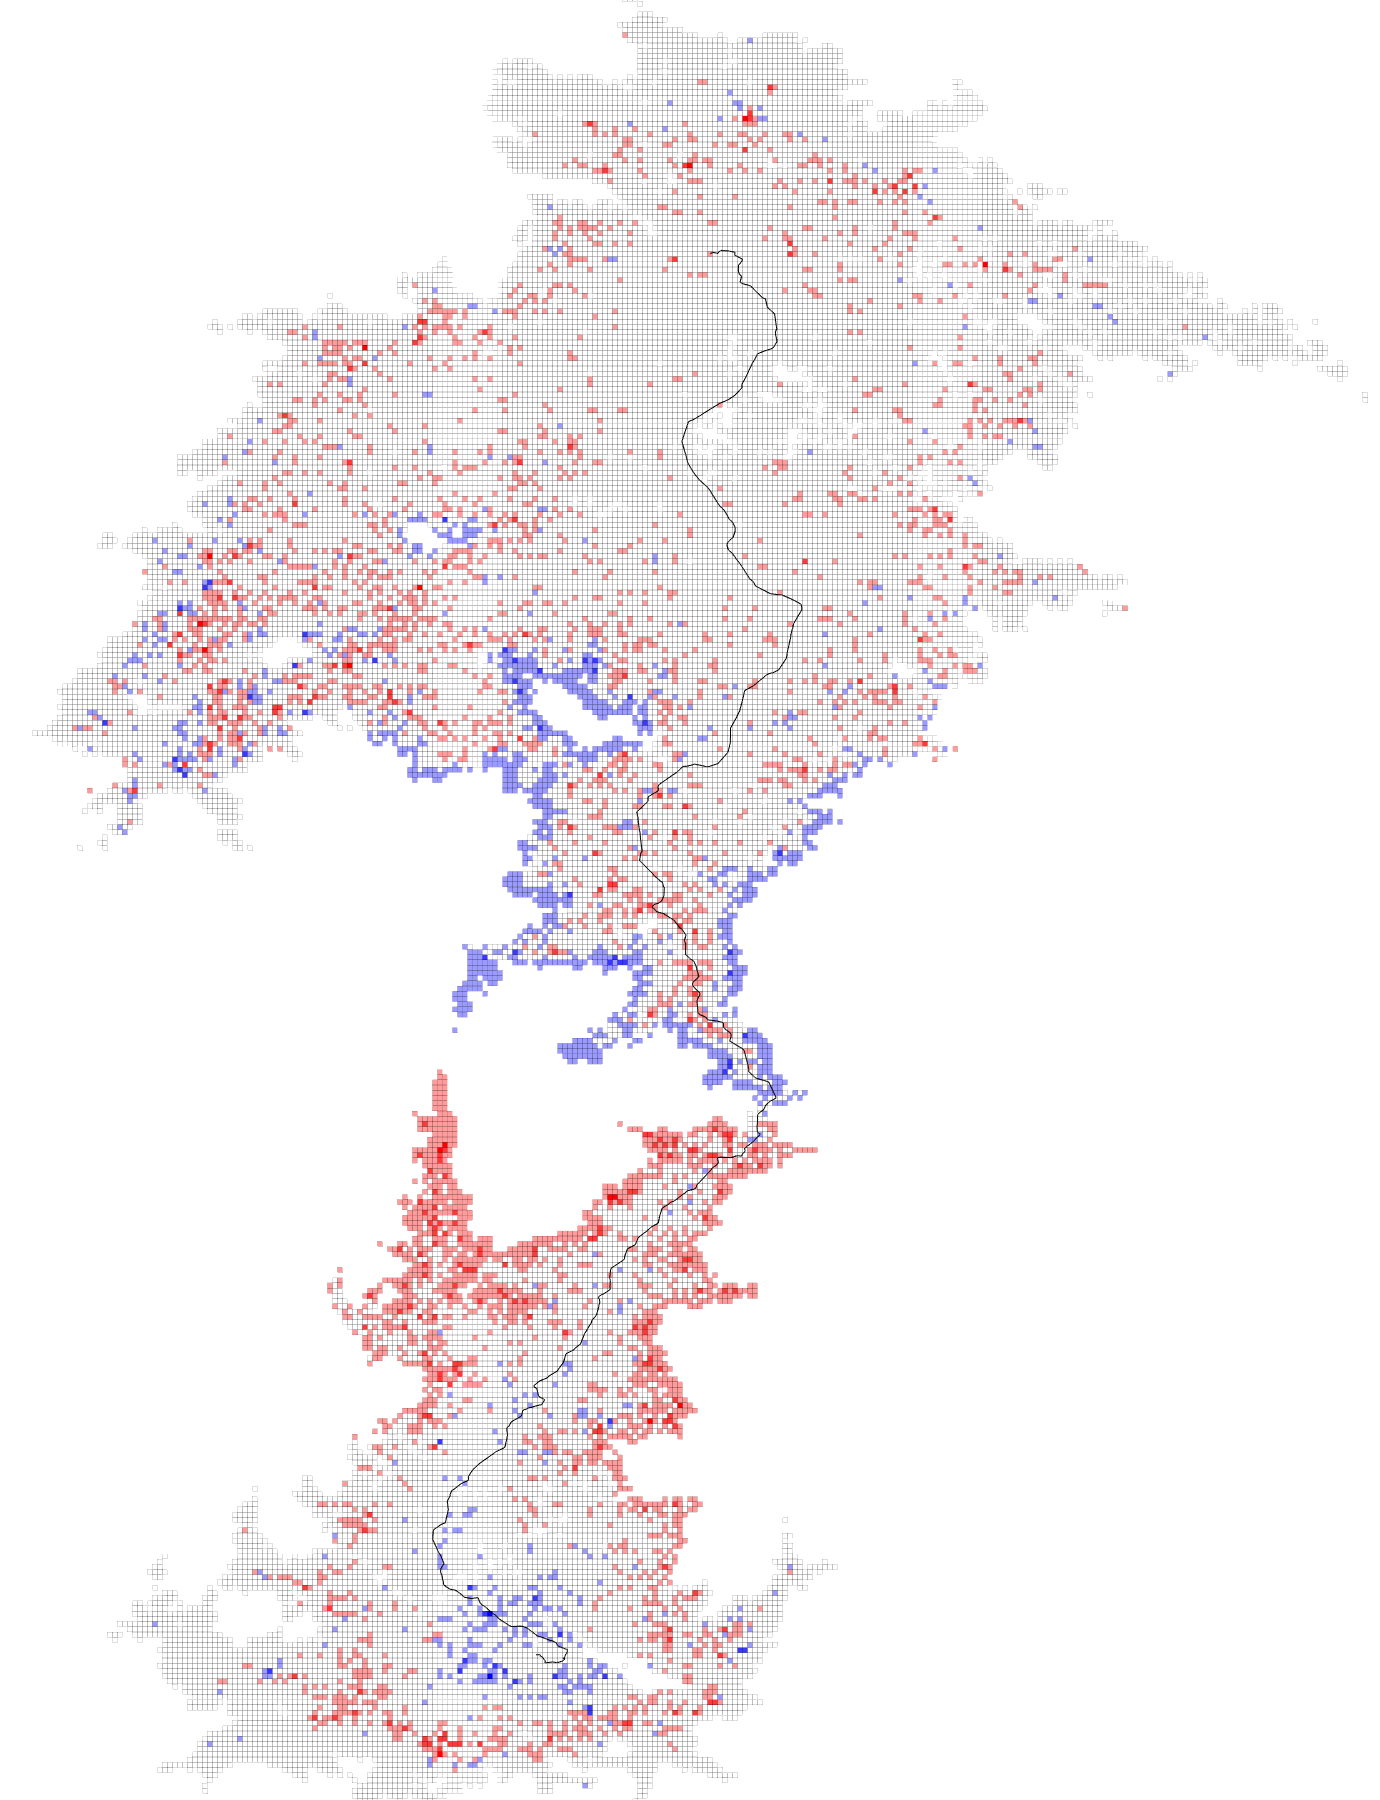
\includegraphics[width=\textwidth]{Images/vis-compare-colored.png}
\caption[]{Showing only the difference of tile loads. Red colors have been loaded more often by the first algorithm, blue colored tiles by the second algorithm. Those tiles colored white, have been loaded equally by both algorithms.}
\label{fig:difference}
\end{figure}

In  \Cref{fig:difference} we can the comparisson between an algorithm (red) and its variation (blue).
Because of the red and blue bordes of displayed graph we recognize that the search space slightly changed.
In genereal the visualization has more red than blue tiles and therefore the variation of the algorithm seems to be an improvement in this case.
Beside the shifted search space there is another area that has a noticeable accumulation of blue tiles around the target in the lower half of them visualization.
After a closer look on this we figgured out, that when the affected area is explored the biggest part of the cache is used for tiles in the upper part of graph.
This leads to more reloading in the lower part of the graph.
Hence we were able to fix this misbehaviour and made the cache aviable when it was needed in the lower part.


\section{Miscellaneous}

In this section, we will take a look on the visualization we have just build and think about some additional features.
For routes with a bigger distance, as for example in \Cref{fig:reload_coloring_hsv}, we had to realize, that even the high-level visualization, that displays only the tiles, has the issue that single elements, as in this case the tiles, become quite small.
Therefore we added a zoom feature to the visualization.
After having implemented this it was necessary to enable panning as well, as otherwise we would be stuck in the middle of the graph.

\begin{figure}
    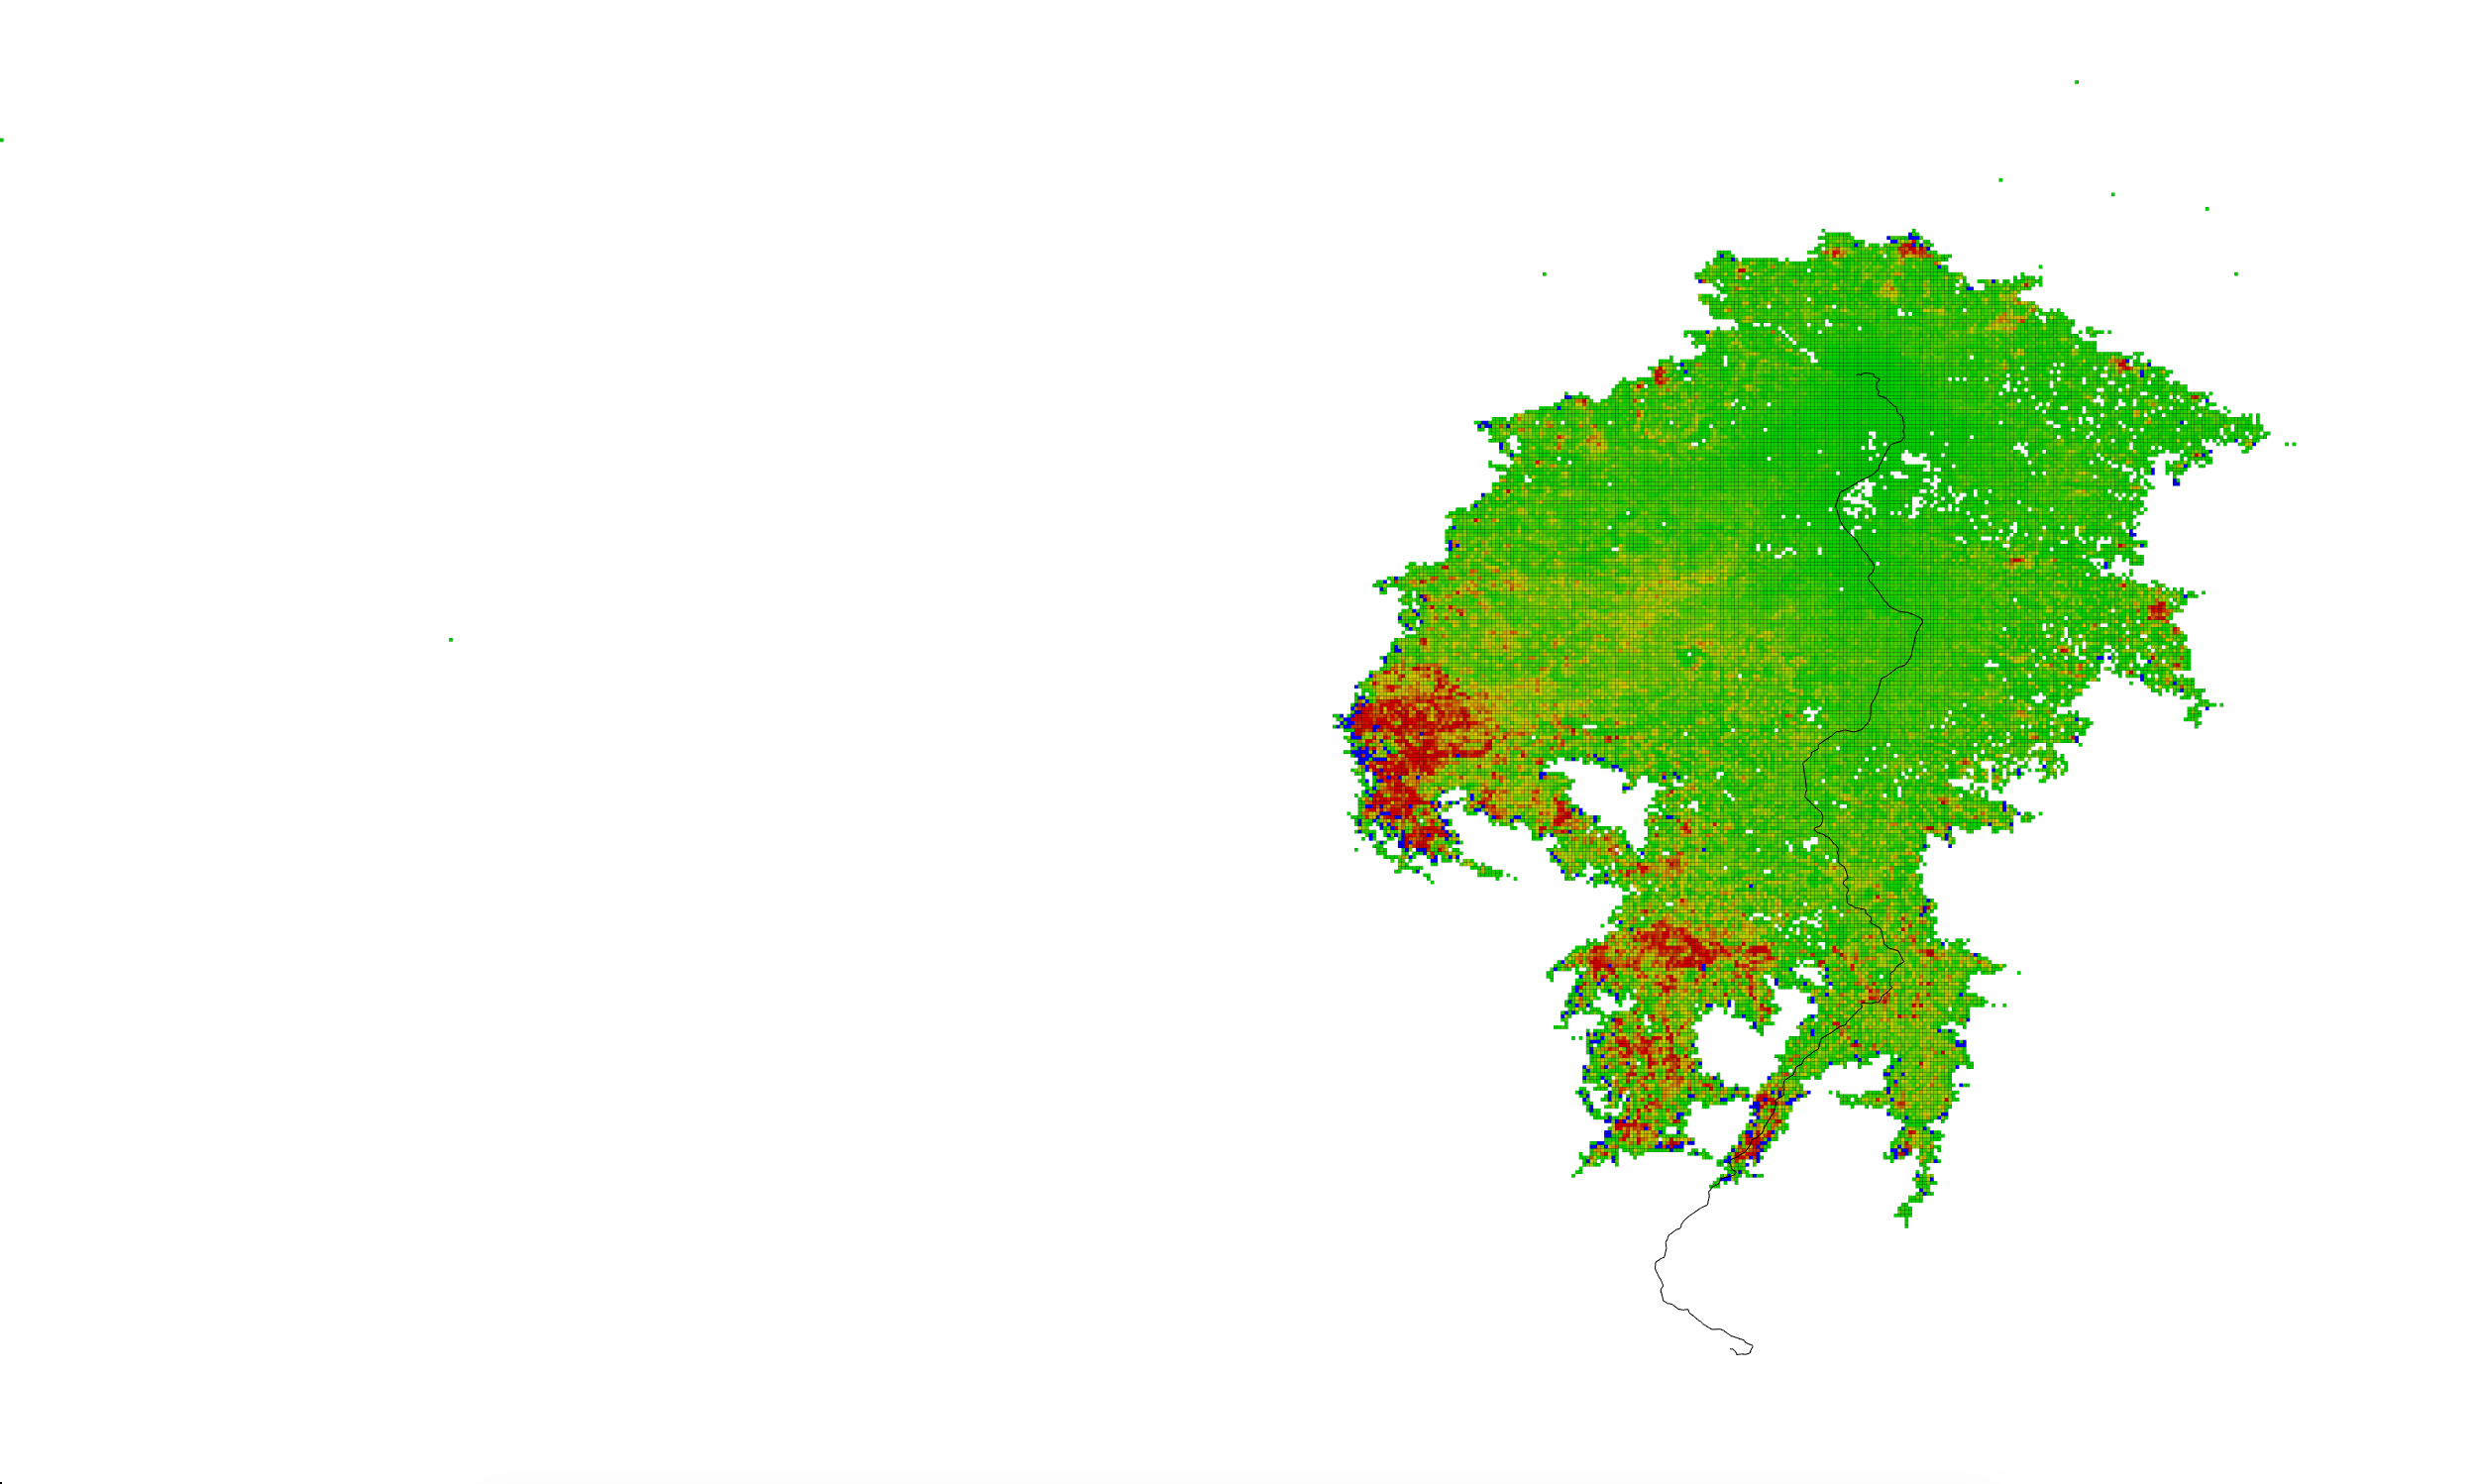
\includegraphics[width=0.5\textwidth]{Images/vis-zoom-small.png}
    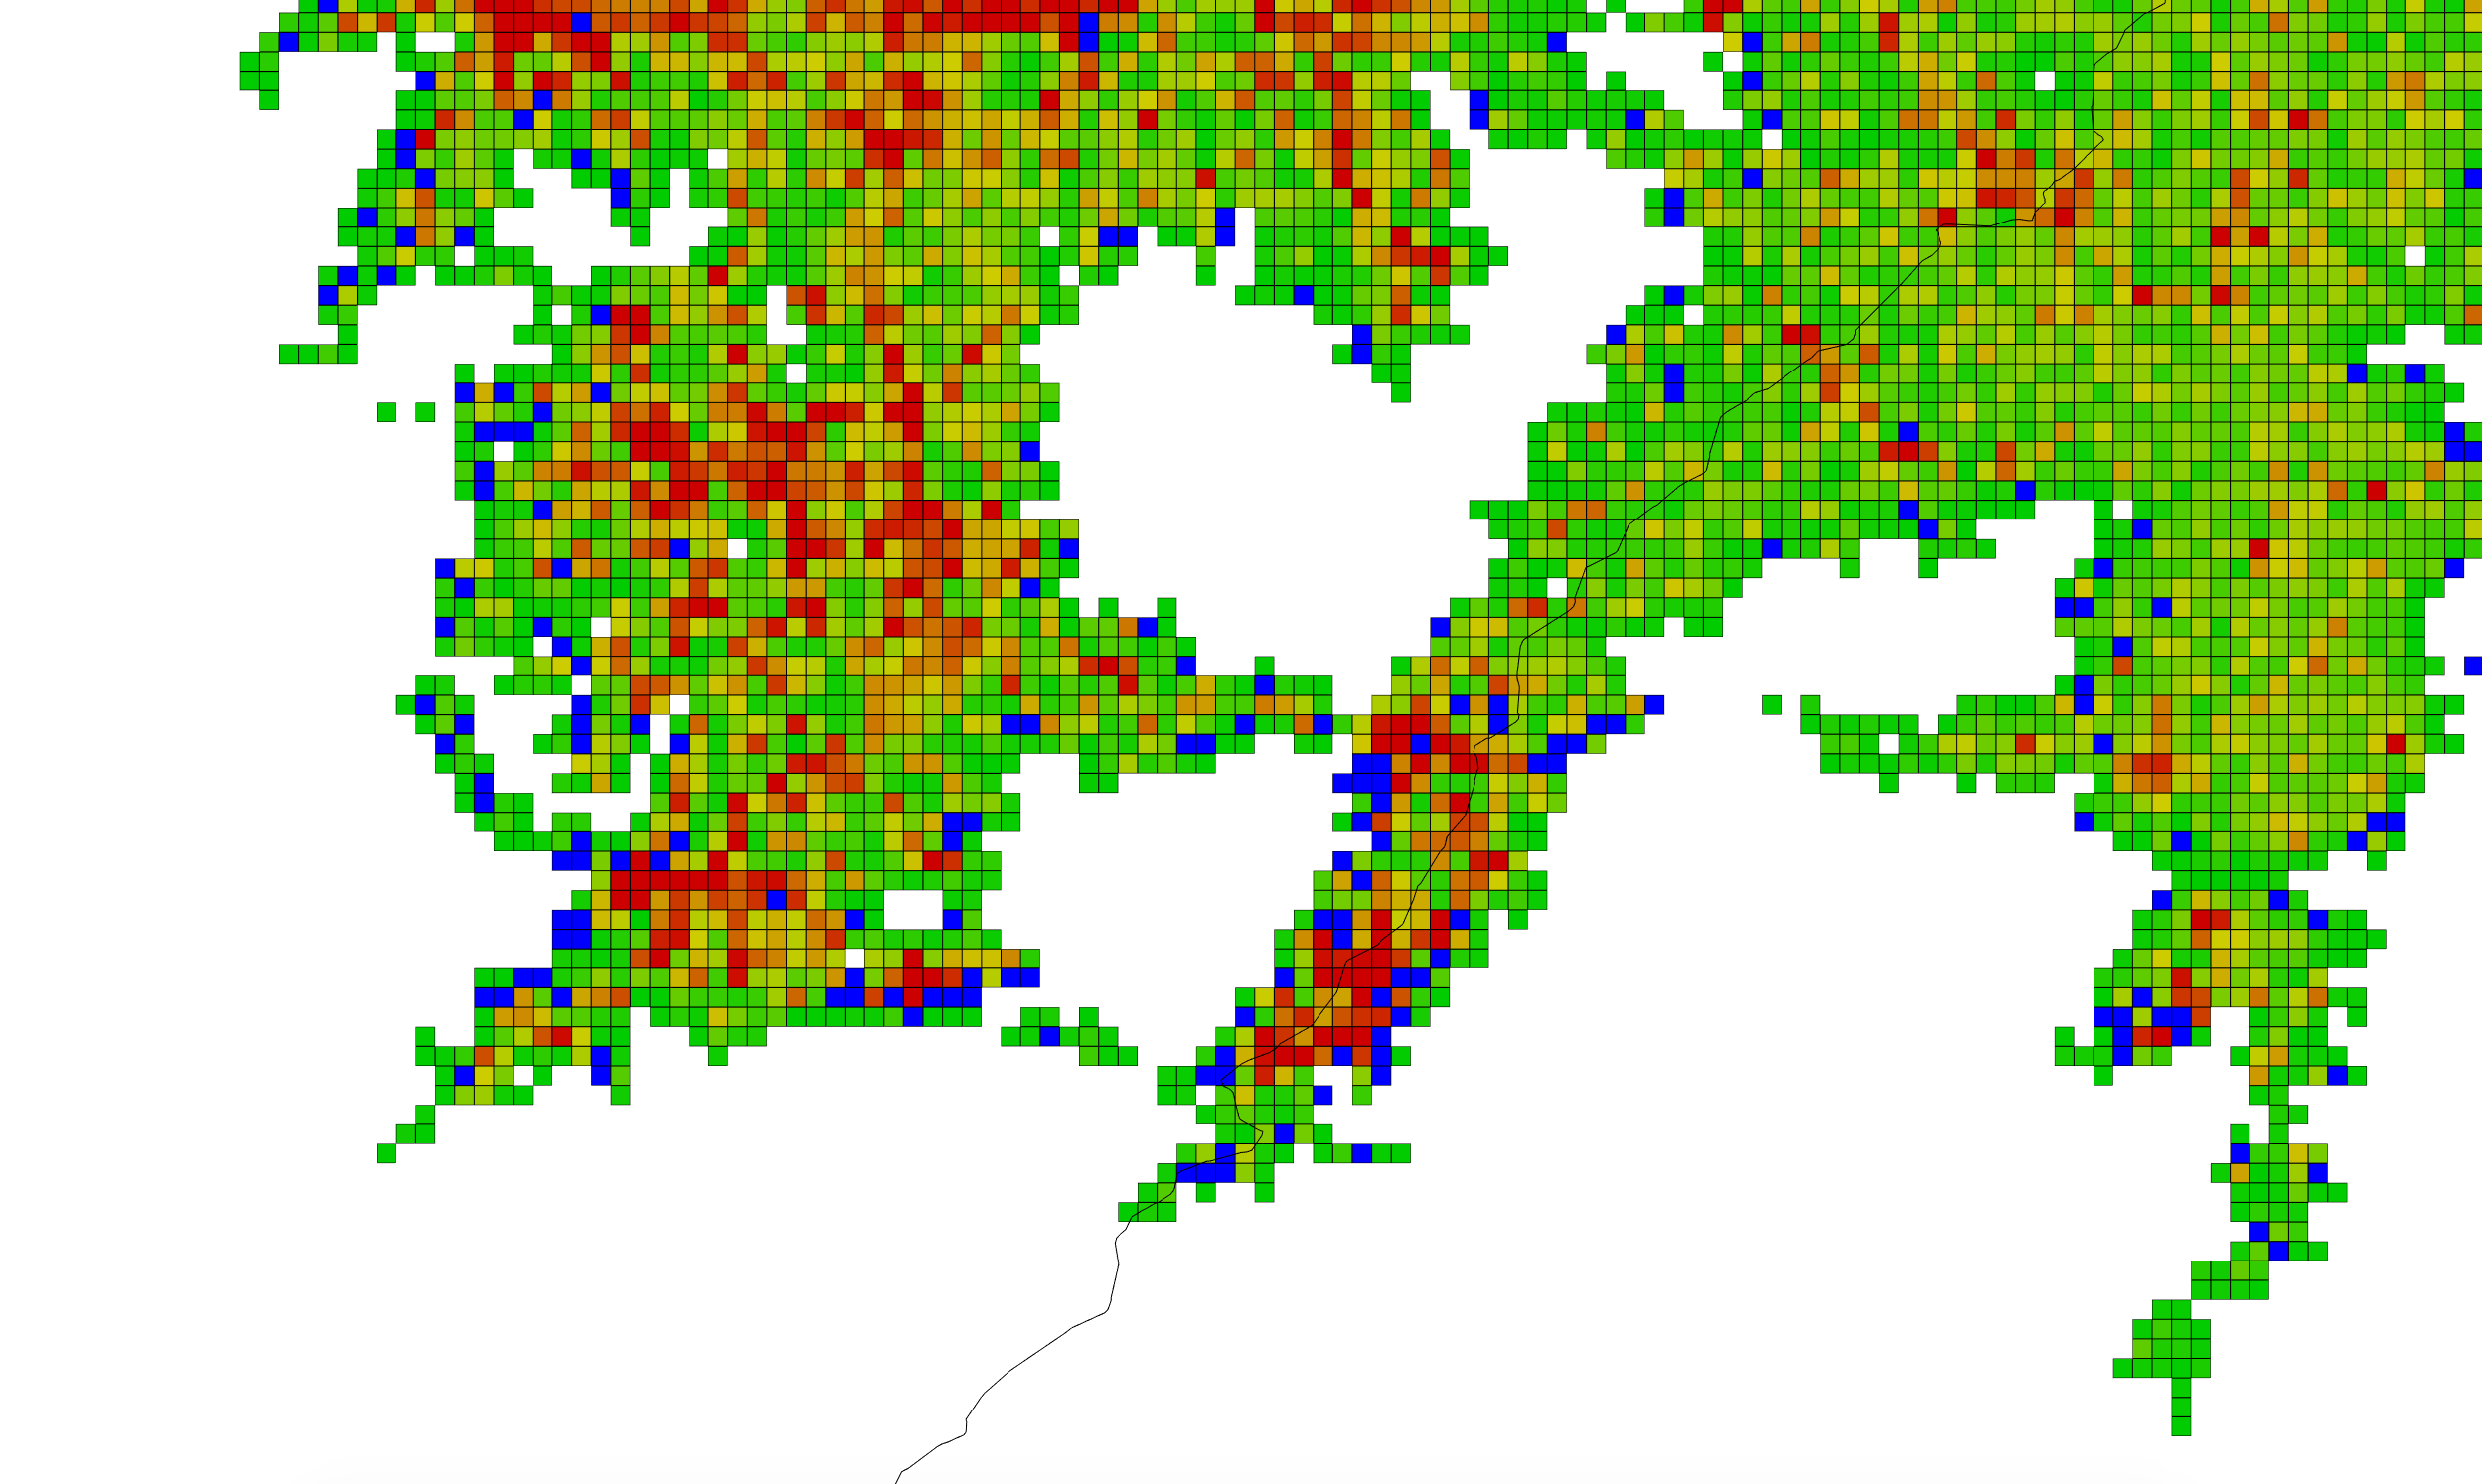
\includegraphics[width=0.5\textwidth]{Images/vis-zoom-large.png}
\caption[]{View on whole graph(left) vz Zoomed view(right)}
\label{fig:zoom}
\end{figure}

We are now able to have a more detailed view on smaller parts of the graph, as we see in \Cref{fig:zoom}.

In \Cref{algorithm}, we described that the edges are not recognizable individually on bigger routes and we, therefore, exluded them from our visualization.
With the possibility of zooming, showing the edges might become a useful feature for our visualization again.
This could, for example, be useful, when we want to understand, why specific tiles are loaded much more than others.
As showing the edges can also make the visualization more confusing and thus distract from the important information, we will make showing the edges optional and make it possible to show and hide them at any point of the visualization.

\begin{figure}
    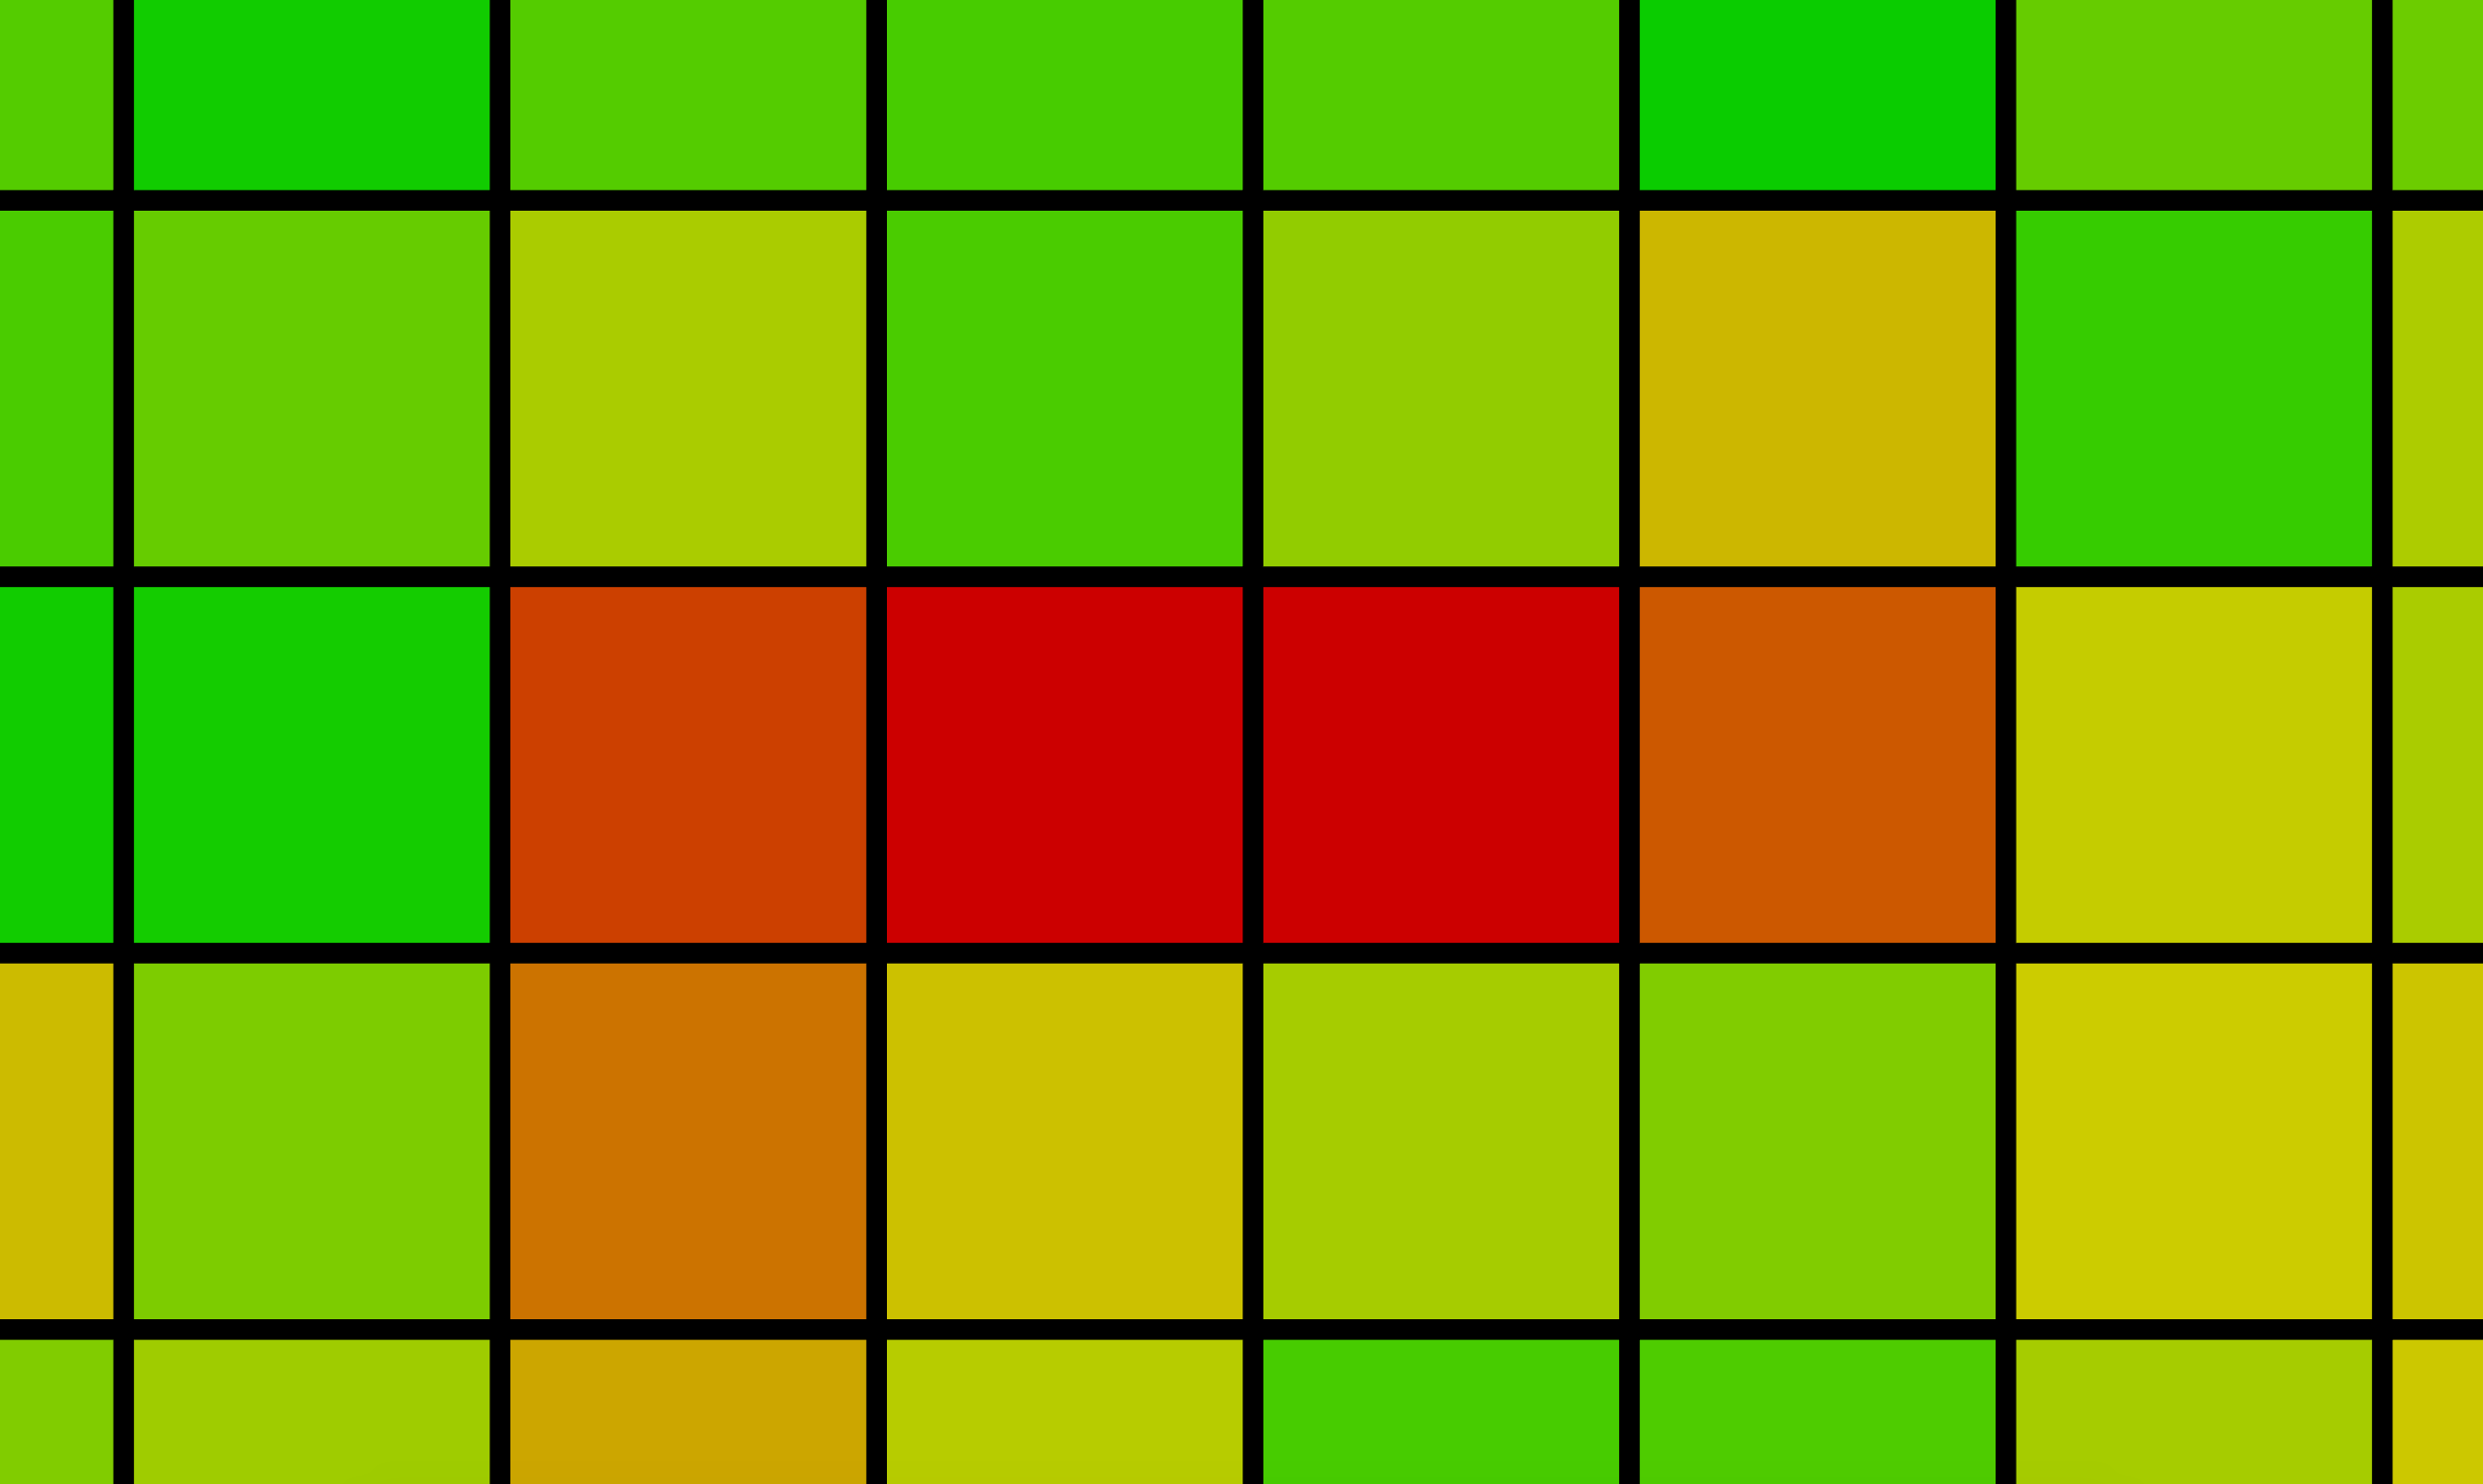
\includegraphics[width=0.5\textwidth]{Images/vis-edges-no.png}
    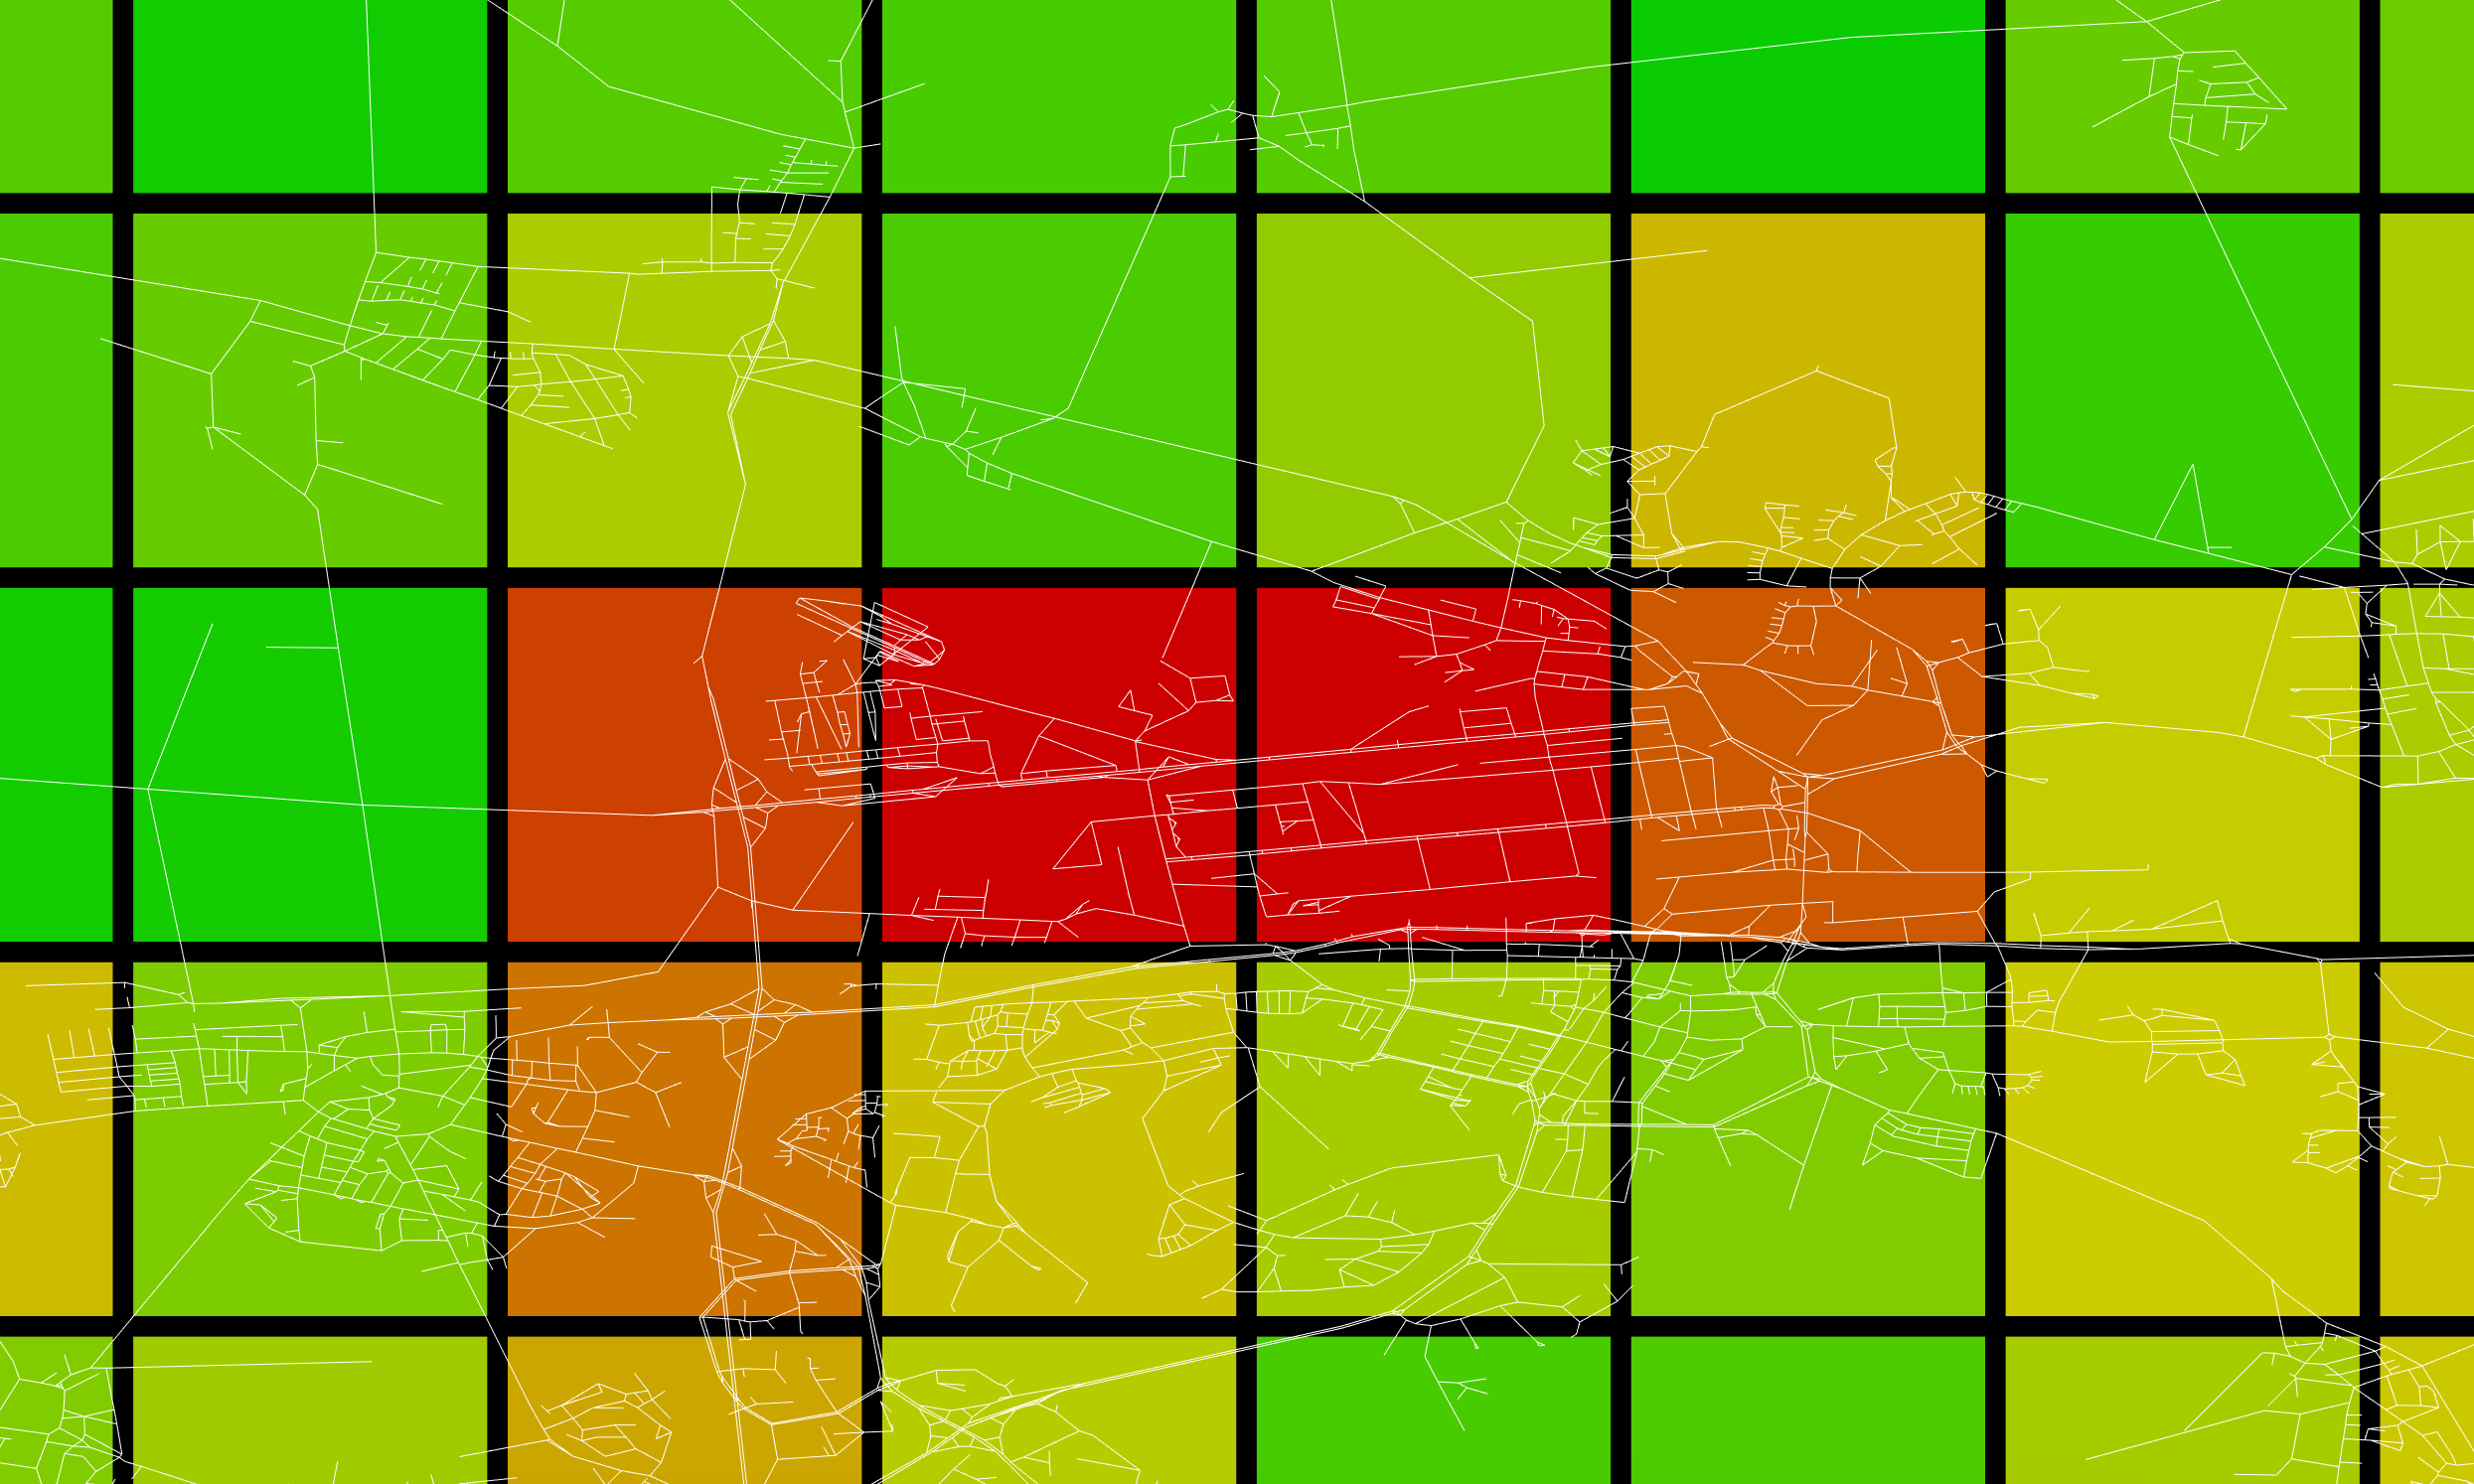
\includegraphics[width=0.5\textwidth]{Images/vis-edges-white.png}
\caption[]{Viewing the graph itself in addition to the tiles.}
\label{fig:white edges}
\end{figure}

Showing the edges helps to understand why some tiles in \Cref{fig:white edges} are loaded more often than others.
The tiles with more reloadings have a high amount of nodes and edges.
Nevertheless, there are also other tiles with many nodes and edges, which are loaded less often.
Therefore we decided to use the colored edges described in \Cref{graph} and thereby also include information about the speed.

\begin{figure}
    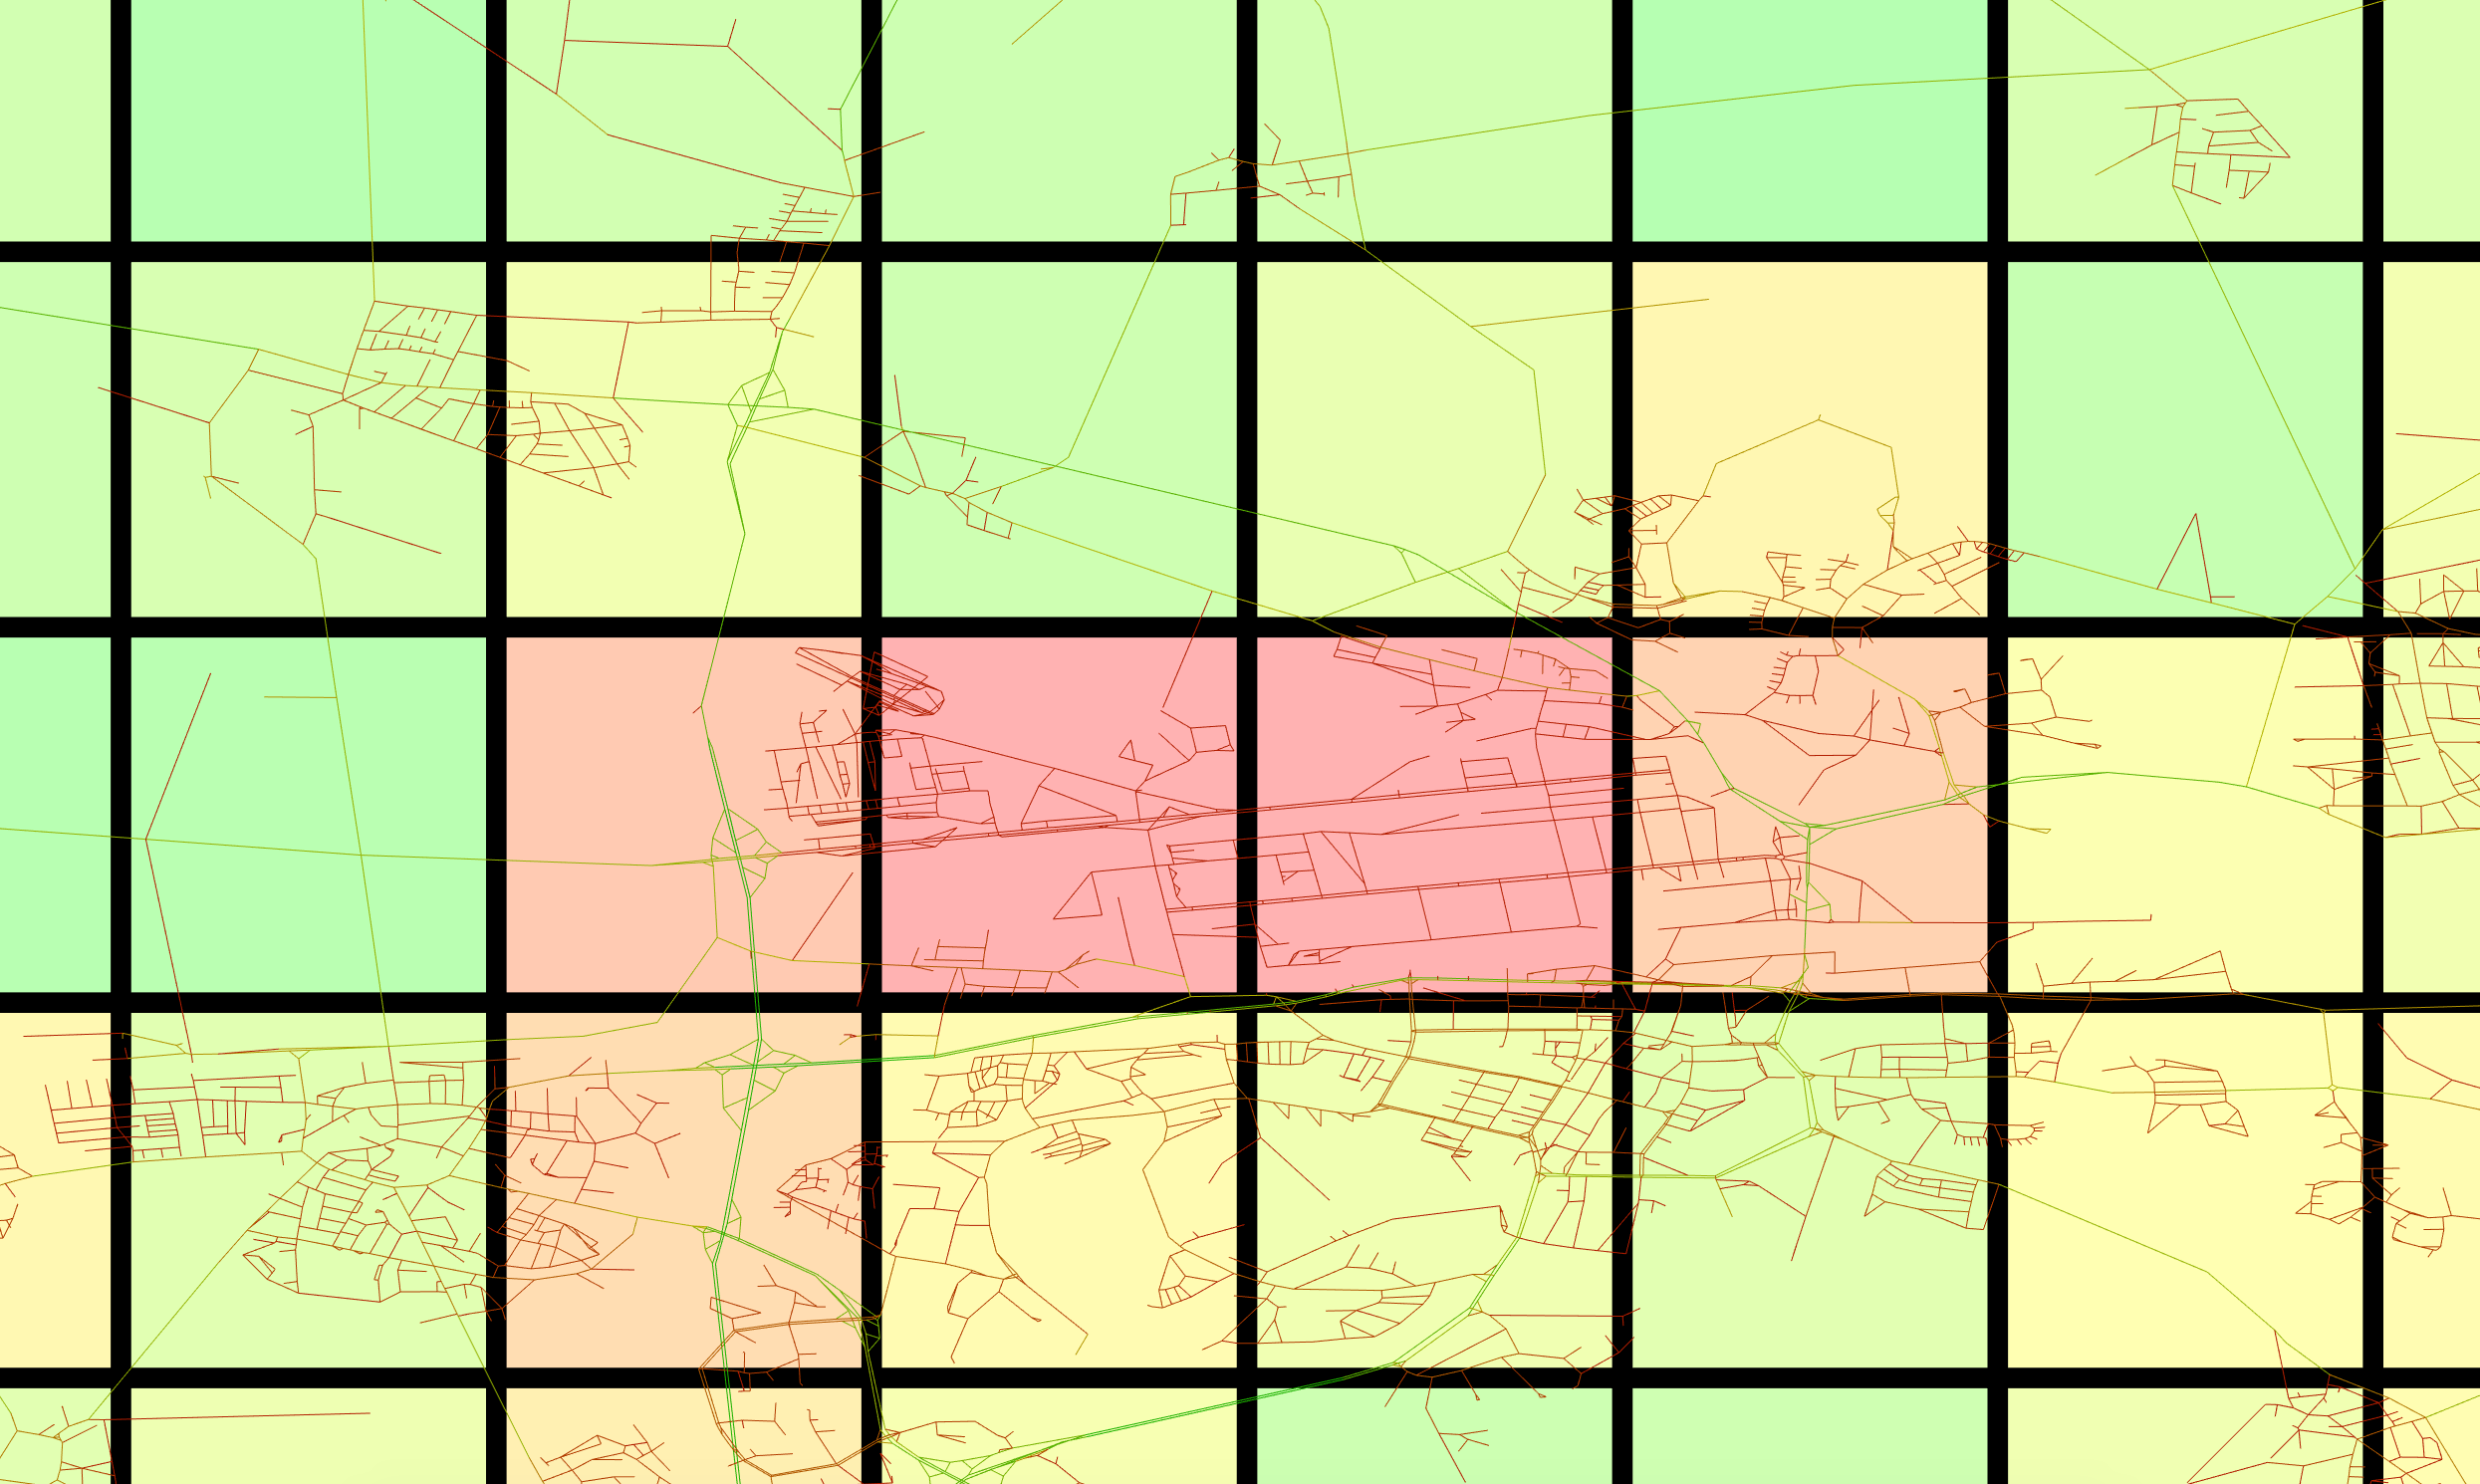
\includegraphics[width=\textwidth]{Images/vis-edges-hsv.png}
\caption[]{Speed based color scheeme. For showing the edges more clearly the tiles are colored brighter.}
\label{fig:colored edges}
\end{figure}

In \Cref{fig:colored edges} we can now see that in the tiles that are loaded more often there are not only many edges, but those with a very small speed.
The surrounding and less loaded tiles allow a higher speed in general.

An other feature we needed, after the algorithms became better was to be able to adjust the level of coloring reloaded, as it is otherwise not possible to find the tiles that have been loaded more often when the most loaded tiles have only been loaded 5 times.
We decided to make this level adjustable while the visualization is running.

\begin{figure}
    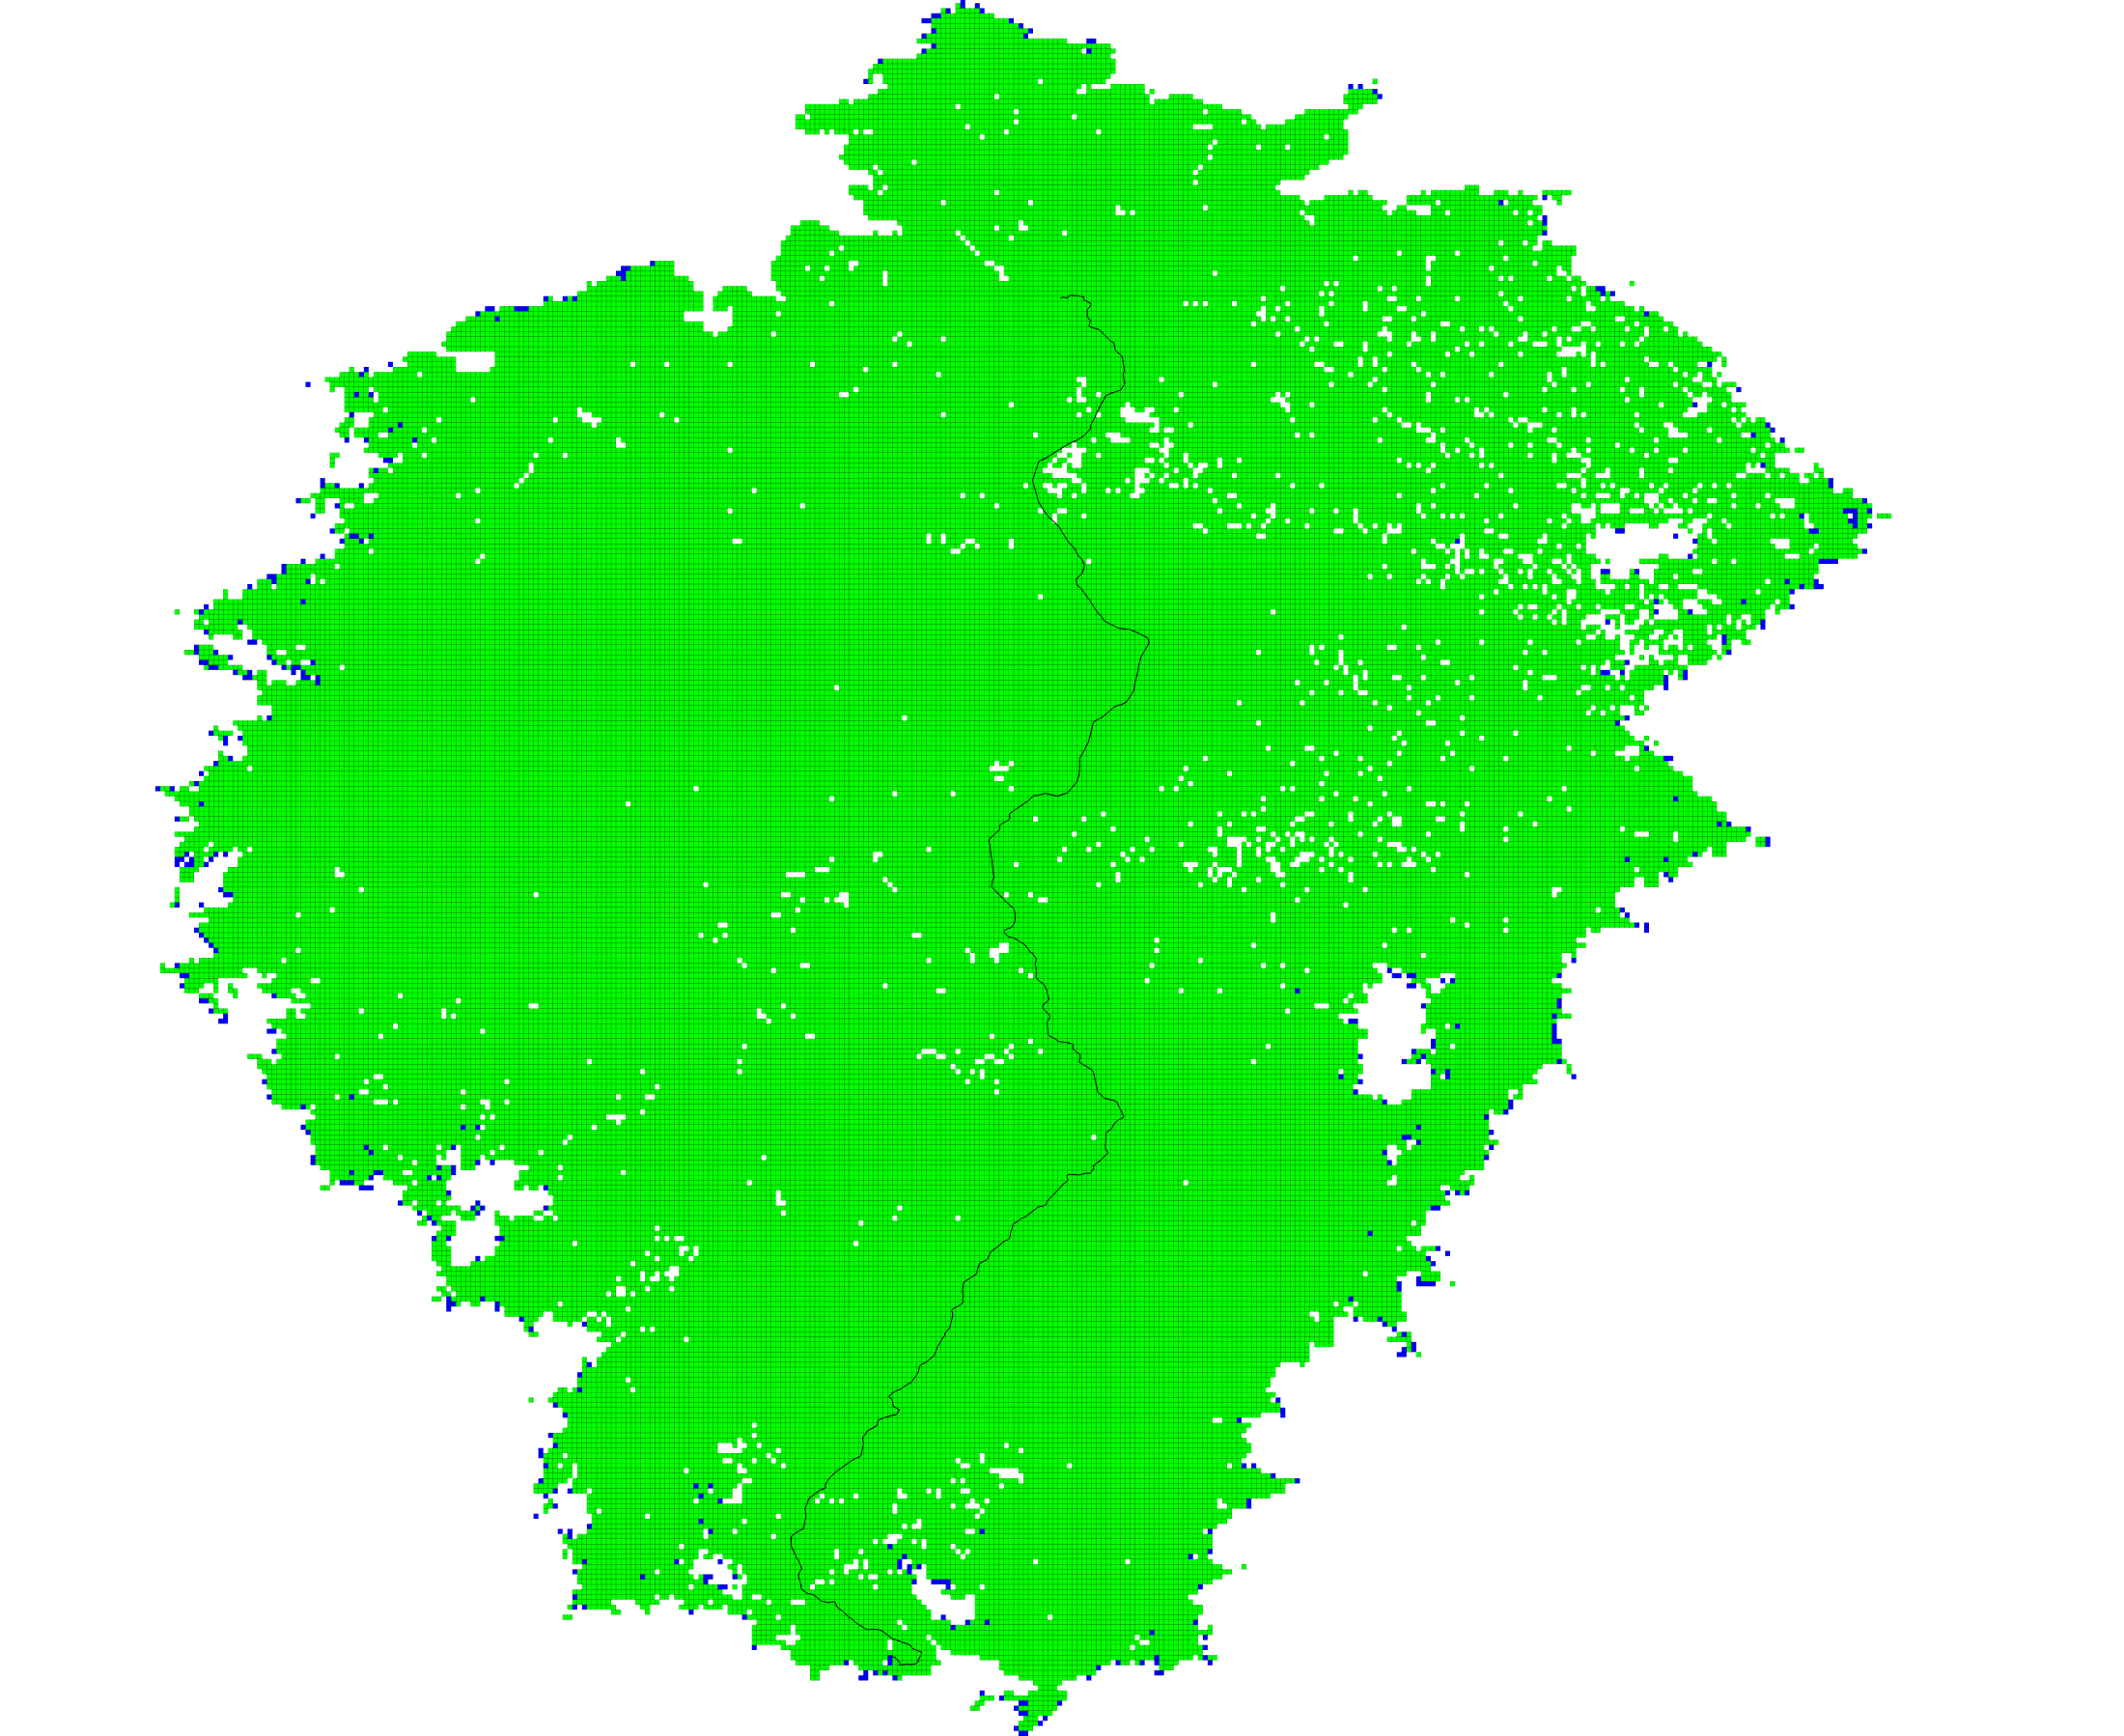
\includegraphics[width=0.5\textwidth]{Images/vis-no-factor.png}
  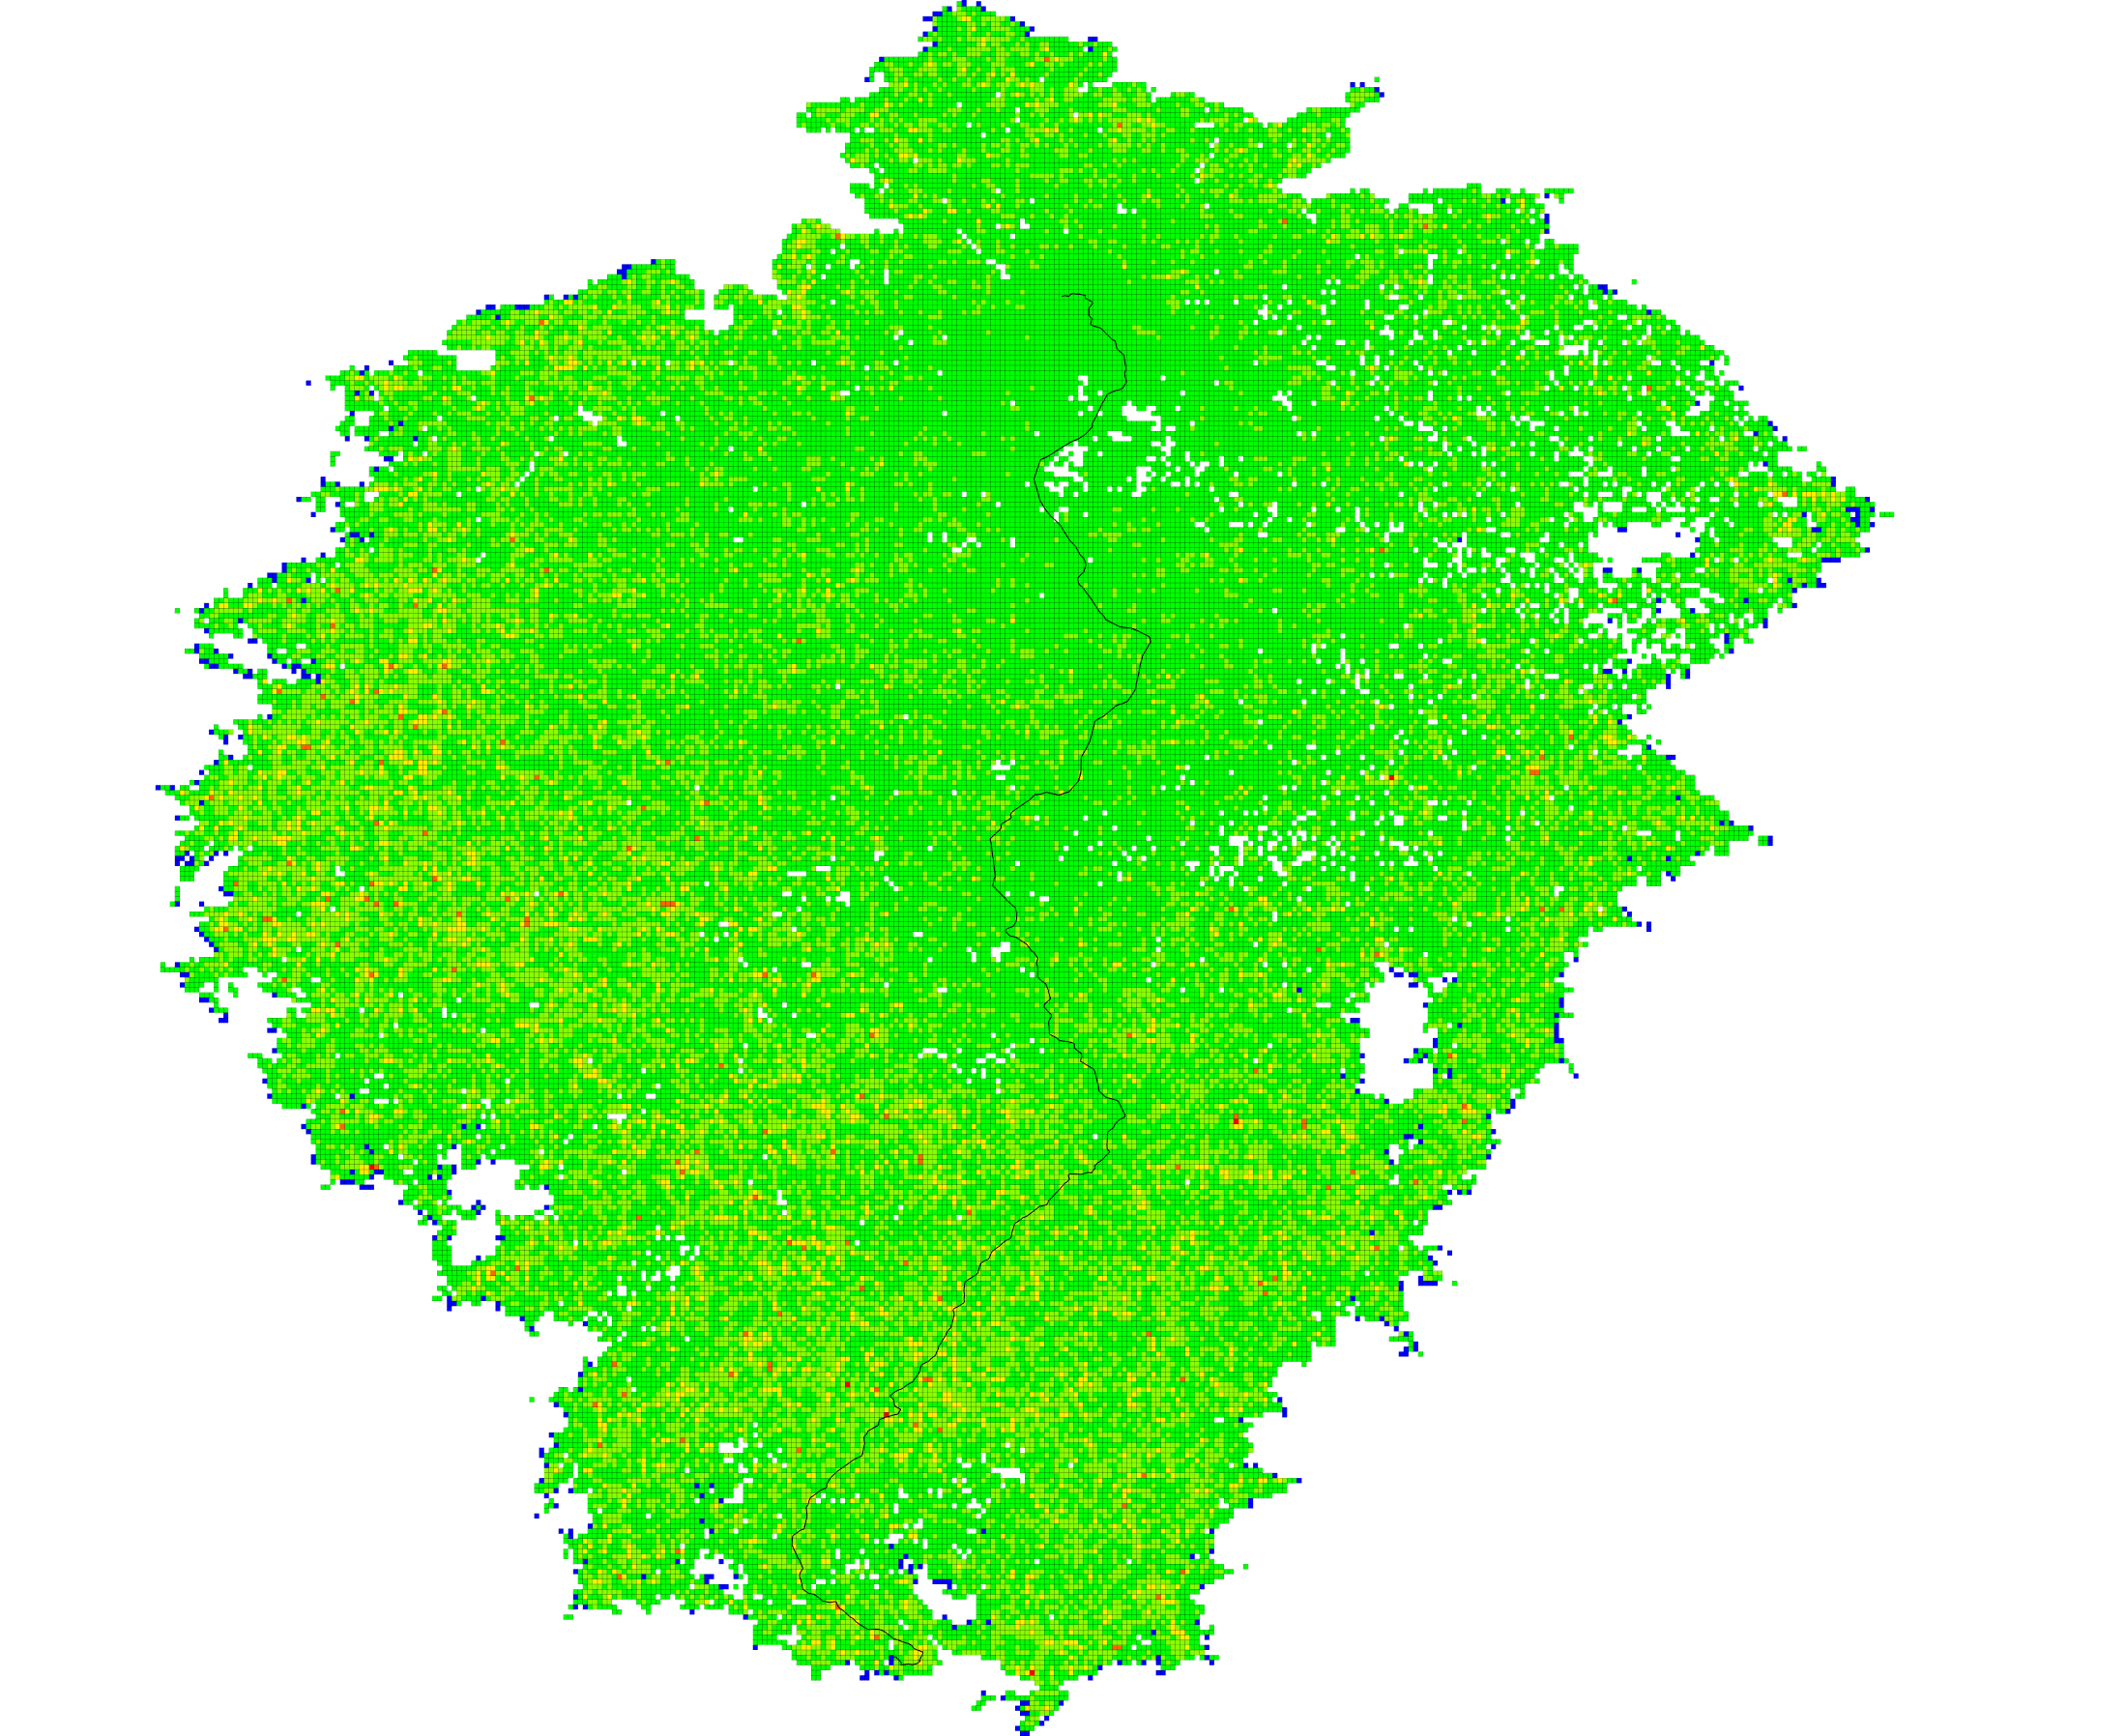
\includegraphics[width=0.5\textwidth]{Images/vis-factor.png}
\caption[]{A well performing algorithm with normal coloring (left) and a more sensitive coloring (right).}
\label{fig:factor}
\end{figure}

By increasing the coloring of reloads in \Cref{fig:factor} we are now able to recognize weaknesses even on highly developed algorithm.

\chapter{Conclusion and Outlook}

The development of algorithms is a complex process.
Therefore, visualizations can highly improve this process and enable the researchers to reach a bigger understanding on weaknesses and serve as a basis for discussions.

Due to finiteness of available space on the screen, the amount of elements that can be displayed without losing comprehensibility is limited as well.
Especially on bigger graphs, this limit raises problems and a certain level of abstraction needs to be found.
Therefore, elements need to be assessed with regard to their importance to the kind of algorithm and the way the algorithms should be improved.
Another aspect that needs to be considered is the amount of the specific element.
In our case for example we decided not to show every single edge as the relation between importance and their amount is disproportionate.
On the contrary the tiles play a big role for the algorithm and their total amount is quite low.

The decision which elements to show strongly depends on the role of the elements for the algorithm.
In our case the decision of which elements we want to show, was quite straightforward, as the most important elements where not that frequent.
On algorithms on which very frequent elements have a big impact it might me necessary to introduce a new element as an abstraction of others.


% In our case the edges are insofar relevant, as they are a fundermental part of the graph, but for the development of the algorithm they do not play a major role.
% On the other hand the amount of edges is huge.
% Those factors make those methods that use the edges for showing the process of the algorithm less sensemaking because of their lack of clairity.
% Nevertheless in combination with the zoom feature displaying edges becomes reasonable, as zooming in reduces the amount of displayed elements on the screen and therefore enables a more detailed view.
%
% On the contrary the total amount of tiles is in a reasonable relation to their importance for the algorithm.
% In addition the rectangular representation of the tiles turned out to be a good canvas for presenting information about the cache and the performance of the displayed algorithm.

%\begin{itemize}
%     \item verschiedene Projektionen
%     \item different layers
%     \item gerichtete edges
% \end{itemize}

% References
\renewcommand*{\bibname}{References}
\bibliographystyle{abbrvnat}
\bibliography{Files/References}


\chapter*{Independence Declaration}
\addcontentsline{toc}{chapter}{Declaration of Authorship}
\thispagestyle{empty}

I hereby declare that the thesis submitted is my own unaided work. All direct or indirect sources used are acknowledged as references.\vspace{2 ex}

Potsdam, \today\\[6 ex]

\begin{flushleft}
    \begin{tabular}{p{5cm}}
        \hline
        \centering\footnotesize\printAuthor
    \end{tabular}
\end{flushleft}


\end{document}
